\documentclass[11pt,english,doublespacing,liststotoc,tocbibind,headsepline]{MastersDoctoralThesis}\usepackage[]{graphicx}\usepackage[]{color}
% maxwidth is the original width if it is less than linewidth
% otherwise use linewidth (to make sure the graphics do not exceed the margin)
\makeatletter
\def\maxwidth{ %
  \ifdim\Gin@nat@width>\linewidth
    \linewidth
  \else
    \Gin@nat@width
  \fi
}
\makeatother

\definecolor{fgcolor}{rgb}{0.345, 0.345, 0.345}
\newcommand{\hlnum}[1]{\textcolor[rgb]{0.686,0.059,0.569}{#1}}%
\newcommand{\hlstr}[1]{\textcolor[rgb]{0.192,0.494,0.8}{#1}}%
\newcommand{\hlcom}[1]{\textcolor[rgb]{0.678,0.584,0.686}{\textit{#1}}}%
\newcommand{\hlopt}[1]{\textcolor[rgb]{0,0,0}{#1}}%
\newcommand{\hlstd}[1]{\textcolor[rgb]{0.345,0.345,0.345}{#1}}%
\newcommand{\hlkwa}[1]{\textcolor[rgb]{0.161,0.373,0.58}{\textbf{#1}}}%
\newcommand{\hlkwb}[1]{\textcolor[rgb]{0.69,0.353,0.396}{#1}}%
\newcommand{\hlkwc}[1]{\textcolor[rgb]{0.333,0.667,0.333}{#1}}%
\newcommand{\hlkwd}[1]{\textcolor[rgb]{0.737,0.353,0.396}{\textbf{#1}}}%
\let\hlipl\hlkwb

\usepackage{framed}
\makeatletter
\newenvironment{kframe}{%
 \def\at@end@of@kframe{}%
 \ifinner\ifhmode%
  \def\at@end@of@kframe{\end{minipage}}%
  \begin{minipage}{\columnwidth}%
 \fi\fi%
 \def\FrameCommand##1{\hskip\@totalleftmargin \hskip-\fboxsep
 \colorbox{shadecolor}{##1}\hskip-\fboxsep
     % There is no \\@totalrightmargin, so:
     \hskip-\linewidth \hskip-\@totalleftmargin \hskip\columnwidth}%
 \MakeFramed {\advance\hsize-\width
   \@totalleftmargin\z@ \linewidth\hsize
   \@setminipage}}%
 {\par\unskip\endMakeFramed%
 \at@end@of@kframe}
\makeatother

\definecolor{shadecolor}{rgb}{.97, .97, .97}
\definecolor{messagecolor}{rgb}{0, 0, 0}
\definecolor{warningcolor}{rgb}{1, 0, 1}
\definecolor{errorcolor}{rgb}{1, 0, 0}
\newenvironment{knitrout}{}{} % an empty environment to be redefined in TeX

\usepackage{alltt}
%%%%%%%%%%%%%%%%%%%%%%%%%%%%%%%%%%%%%%%%%
% Masters/Doctoral Thesis
% LaTeX Template
% Version 2.5 (27/8/17)
%
% This template was downloaded from:
% http://www.LaTeXTemplates.com
%
% Version 2.x major modifications by:
% Vel (vel@latextemplates.com)
%
% This template is based on a template by:
% Steve Gunn (http://users.ecs.soton.ac.uk/srg/softwaretools/document/templates/)
% Sunil Patel (http://www.sunilpatel.co.uk/thesis-template/)
%
% Template license:
% CC BY-NC-SA 3.0 (http://creativecommons.org/licenses/by-nc-sa/3.0/)
%
%%%%%%%%%%%%%%%%%%%%%%%%%%%%%%%%%%%%%%%%%

%----------------------------------------------------------------------------------------
%   PACKAGES AND OTHER DOCUMENT CONFIGURATIONS
%----------------------------------------------------------------------------------------

% \documentclass[
% 11pt, % The default document font size, options: 10pt, 11pt, 12pt
% %oneside, % Two side (alternating margins) for binding by default, uncomment to switch to one side
% english, % ngerman for German
% doublespacing,
% % singlespacing, % Single line spacing, alternatives: onehalfspacing or doublespacing
% % draft, % Uncomment to enable draft mode (no pictures, no links, overfull hboxes indicated)
% %nolistspacing, % If the document is onehalfspacing or doublespacing, uncomment this to set spacing in lists to single
% liststotoc, % Uncomment to add the list of figures/tables/etc to the table of contents
% tocbibind,
% %toctotoc, % Uncomment to add the main table of contents to the table of contents
% %parskip, % Uncomment to add space between paragraphs
% %nohyperref, % Uncomment to not load the hyperref package
% headsepline, % Uncomment to get a line under the header
% %chapterinoneline, % Uncomment to place the chapter title next to the number on one line
% %consistentlayout, % Uncomment to change the layout of the declaration, abstract and acknowledgements pages to match the default layout
% ]{MastersDoctoralThesis} % The class file specifying the document structure

\usepackage[utf8]{inputenc} % Required for inputting international characters
\usepackage[T1]{fontenc} % Output font encoding for international characters

\usepackage{mathpazo} % Use the Palatino font by default
%\usepackage{bookman}

\usepackage{amssymb}
\usepackage{enumerate}

\cslet{blx@noerroretextools}\empty
\usepackage[backend=bibtex,style=authoryear-comp,natbib=true,giveninits]{biblatex} % Use the bibtex backend with the authoryear citation style (which resembles APA)
\DeclareNameAlias{sortname}{family-given}

\addbibresource{reflist.bib} % The filename of the bibliography

\usepackage[autostyle=true]{csquotes} % Required to generate language-dependent quotes in the bibliography

\usepackage{amsmath,amsfonts}

\usepackage{listings}
\usepackage{courier}
\lstset{basicstyle=\footnotesize\ttfamily,breaklines=true}

%\usepackage[acronym,nonumberlist,toc,nomain]{glossaries} %Load glossaries package
\usepackage[acronym,nonumberlist,toc,nomain]{glossaries-extra}
\makeglossaries
\GlsXtrEnableEntryUnitCounting
 {abbreviation}% list of categories to use entry counting
 {3}
 {chapter}

\usepackage{soul}
\newcommand{\note}[2][]{{\ul{#1}~\footnotesize\textcolor{blue}{\emph{[#2]}}}}

% because I always forget to use \citet
\let\cite\citet

\newacronym{avl}{AVL}{automatic vehicle location}
\newacronym{rti}{RTI}{real-time information}
\newacronym[longplural=estimated times of arrival]{eta}{ETA}{estimated time of arrival}
\newacronym{api}{API}{application programming language}
\newacronym{gps}{GPS}{global positioning system}


%----------------------------------------------------------------------------------------
%   MARGIN SETTINGS
%----------------------------------------------------------------------------------------

\geometry{
    paper=a4paper, % Change to letterpaper for US letter
    inner=2.5cm, % Inner margin
    outer=3.8cm, % Outer margin
    bindingoffset=.5cm, % Binding offset
    top=1.5cm, % Top margin
    bottom=1.5cm, % Bottom margin
    %showframe, % Uncomment to show how the type block is set on the page
}

%----------------------------------------------------------------------------------------
%   THESIS INFORMATION
%----------------------------------------------------------------------------------------

\thesistitle{Improving the prediction of bus arrival using real-time network state} % Your thesis title, this is used in the title and abstract, print it elsewhere with \ttitle
\supervisor{Professor Thomas \textsc{Lumley}} % Your supervisor's name, this is used in the title page, print it elsewhere with \supname
\examiner{} % Your examiner's name, this is not currently used anywhere in the template, print it elsewhere with \examname
\degree{Doctor of Philosophy} % Your degree name, this is used in the title page and abstract, print it elsewhere with \degreename
\author{Tom Mitchell \textsc{Elliott}} % Your name, this is used in the title page and abstract, print it elsewhere with \authorname
\addresses{} % Your address, this is not currently used anywhere in the template, print it elsewhere with \addressname

\subject{Statistics} % Your subject area, this is not currently used anywhere in the template, print it elsewhere with \subjectname
\keywords{} % Keywords for your thesis, this is not currently used anywhere in the template, print it elsewhere with \keywordnames
\university{University of Auckland} % Your university's name and URL, this is used in the title page and abstract, print it elsewhere with \univname
\department{Department of Statistics} % Your department's name and URL, this is used in the title page and abstract, print it elsewhere with \deptname
\group{\href{http://researchgroup.university.com}{Research Group Name}} % Your research group's name and URL, this is used in the title page, print it elsewhere with \groupname
\faculty{Faculty of Science} % Your faculty's name and URL, this is used in the title page and abstract, print it elsewhere with \facname

\AtBeginDocument{
\hypersetup{pdftitle=\ttitle} % Set the PDF's title to your title
\hypersetup{pdfauthor=\authorname} % Set the PDF's author to your name
\hypersetup{pdfkeywords=\keywordnames} % Set the PDF's keywords to your keywords
}

\usepackage{hyperref}
\usepackage[noabbrev]{cleveref}
% \usepackage{autonum}

\usepackage{subfig}

\usepackage{showlabels}
\renewcommand{\showlabelfont}{\tiny}
% \usepackage{showkeys}

%\usepackage{perpage} %the perpage package
%\MakePerPage{footnote}
\usepackage[symbol]{footmisc}
\renewcommand{\thefootnote}{\arabic{footnote}}
\IfFileExists{upquote.sty}{\usepackage{upquote}}{}
\begin{document}

\frontmatter % Use roman page numbering style (i, ii, iii, iv...) for the pre-content pages

\pagestyle{plain} % Default to the plain heading style until the thesis style is called for the body content

%----------------------------------------------------------------------------------------
%   TITLE PAGE
%----------------------------------------------------------------------------------------

\begin{titlepage}
\begin{center}

\vspace*{.06\textheight}
{\scshape\LARGE \univname\par}\vspace{1.5cm} % University name
\textsc{\Large Doctoral Thesis}\\[0.5cm] % Thesis type

\HRule \\[0.4cm] % Horizontal line
{\huge \bfseries \ttitle\par}\vspace{0.4cm} % Thesis title
\HRule \\[1.5cm] % Horizontal line

% \vspace{2cm}

\Large\authorname % Author name - remove the \href bracket to remove the link

\vfill

\large \textit{A thesis submitted in fulfillment of the requirements %
for the degree of\\ \degreename\ in\ \subjectname, \univname}\\[0.3cm]

\textit{This thesis is for examination purposes only and is confidential %
to the examination process.}

% \univname

% \vfill
\vspace{1cm}
{\large April 2020}%\\[4cm] % Date
%\includegraphics{Logo} % University/department logo - uncomment to place it

\vfill
\end{center}
\end{titlepage}

%----------------------------------------------------------------------------------------
%   DECLARATION PAGE
%----------------------------------------------------------------------------------------

\begin{declaration}
\addchaptertocentry{\authorshipname} % Add the declaration to the table of contents
\noindent I, \authorname, declare that this thesis titled, \enquote{\ttitle} and the work presented in it are my own. I confirm that:

\begin{itemize}
\item This work was done wholly or mainly while in candidature for a research degree at this University.
\item Where any part of this thesis has previously been submitted for a degree or any other qualification at this University or any other institution, this has been clearly stated.
\item Where I have consulted the published work of others, this is always clearly attributed.
\item Where I have quoted from the work of others, the source is always given. With the exception of such quotations, this thesis is entirely my own work.
\item I have acknowledged all main sources of help.
\item Where the thesis is based on work done by myself jointly with others, I have made clear exactly what was done by others and what I have contributed myself.\\
\end{itemize}

\noindent Signed:\\
\rule[0.5em]{25em}{0.5pt} % This prints a line for the signature

\noindent Date:\\
\rule[0.5em]{25em}{0.5pt} % This prints a line to write the date
\end{declaration}

\cleardoublepage

%----------------------------------------------------------------------------------------
%   QUOTATION PAGE
%----------------------------------------------------------------------------------------

\vspace*{0.2\textheight}

\noindent\enquote{\itshape Thanks to my solid academic training, today I can write hundreds of words on virtually any topic without possessing a shred of information, which is how I got a good job in journalism.}\bigbreak

\hfill Dave Barry

%----------------------------------------------------------------------------------------
%   ABSTRACT PAGE
%----------------------------------------------------------------------------------------

\begin{abstract}
\addchaptertocentry{\abstractname} % Add the abstract to the table of contents
The Thesis Abstract is written here (and usually kept to just this page). The page is kept centered vertically so can expand into the blank space above the title too\ldots
\end{abstract}

%----------------------------------------------------------------------------------------
%   ACKNOWLEDGEMENTS
%----------------------------------------------------------------------------------------

\begin{acknowledgements}
\addchaptertocentry{\acknowledgementname} % Add the acknowledgements to the table of contents
The acknowledgments and the people to thank go here, don't forget to include your project advisor\ldots
\end{acknowledgements}

%----------------------------------------------------------------------------------------
%   LIST OF CONTENTS/FIGURES/TABLES PAGES
%----------------------------------------------------------------------------------------

\tableofcontents % Prints the main table of contents

\listoffigures % Prints the list of figures

\listoftables % Prints the list of tables

%----------------------------------------------------------------------------------------
%   ABBREVIATIONS
%----------------------------------------------------------------------------------------

%\glsaddall
\printglossary[type=\acronymtype,title=List of Abbreviations] %Generate List of Abbreviations

%----------------------------------------------------------------------------------------
%   SYMBOLS
%----------------------------------------------------------------------------------------

% plan to remove these
\newcommand{\bB}{\mathbf{B}}
\newcommand{\bbeta}{\boldsymbol\beta}
\newcommand{\bbetahat}{\boldsymbol{\hat\beta}}
\newcommand{\bY}{\boldsymbol Y}
\newcommand{\bX}{\boldsymbol X}
\newcommand{\bx}{\boldsymbol x}
\newcommand{\bz}{\boldsymbol z}
\newcommand{\bbX}{\textbf{X}}



%% new symbol list, better structured

\newcommand{\mat}[1]{\mathbf{#1}}
\renewcommand{\vec}[1]{\boldsymbol{#1}}
\newcommand{\tvec}[1]{\left[#1\right]^\top}
\newcommand{\collect}[1]{\left\{#1\right\}}

\newcommand{\Vtime}{t}
\newcommand{\Vtdiff}{\delta}

\newcommand{\Vobs}{\boldsymbol{y}}
\newcommand{\VobsMat}{\mat Y}
\newcommand{\Vlat}{\phi}
\newcommand{\Vlon}{\lambda}
\newcommand{\Varr}{A}
\newcommand{\Vdep}{D}
\newcommand{\Vdwell}{\tilde\Vdep}

\newcommand{\Vstate}{\bx}
\newcommand{\Vdist}{x}
\newcommand{\Vspeed}{\dot x}
\newcommand{\Vaccel}{\ddot x}
\newcommand{\Vtt}{B}
\newcommand{\Vttobs}{b}
\newcommand{\Vtterr}{e}
\newcommand{\Np}{N}
\newcommand{\Pwt}[1][i]{w^{(#1)}}
\newcommand{\Vtrans}{f}
\newcommand{\Vmeas}{h}
\newcommand{\Vprojf}{g}
\newcommand{\Vproj}[2]{g\left(#1\,|\,#2\right)}
\newcommand{\Viproj}[2]{g^{-1}\left(#1\,|\,#2\right)}
\newcommand{\Vnoise}{\sigma^2}
\newcommand{\GPSerrSD}{\varepsilon}
\newcommand{\GPSerr}{\GPSerrSD^2}
\newcommand{\TUerrSD}{\xi}
\newcommand{\TUerr}{\TUerrSD^2}
\newcommand{\Ppos}{\vec{\tilde Y}}

\newcommand{\Neff}{N_\text{eff}}
\newcommand{\Nthres}{N_\text{thres}}

\newcommand{\Vsegstart}{T}
\newcommand{\Vsegend}{T'}

\newcommand{\vi}[1][i]{^{(#1)}}

\newcommand{\Nstop}{M}
\newcommand{\Nseg}{L}
\newcommand{\Tstopd}{\mathcal{S}}
\newcommand{\Tsegd}{\mathcal{D}}
\newcommand{\Tseglen}{\mathcal{L}}
\newcommand{\Prstop}{\pi}
\newcommand{\mindwell}{\gamma}
\newcommand{\dwell}{\tau}
\newcommand{\dwellvar}{\omega^2}
\newcommand{\Istop}{p}
\newcommand{\pdwell}{d}
\newcommand{\pserve}{\tilde d}
\newcommand{\Print}{\rho}
\newcommand{\intwait}{\nu}
\newcommand{\Iint}{r}
\newcommand{\pwait}{w}
\newcommand{\pcwait}{\tilde w}

\newcommand{\NWtdiff}{\Delta}
\newcommand{\NWstate}{\beta}
\newcommand{\NWstatevar}{\mat{P}}
\newcommand{\NWvar}{\mat{\boldsymbol{\psi}}}
\newcommand{\Rstate}{b}
\newcommand{\Rvar}{v}
\newcommand{\NWnoise}{q}
\newcommand{\NWerr}{\Vtterr}
\newcommand{\NWtransfun}{F}
\newcommand{\NWtrans}{\mat{\NWtransfun}}
\newcommand{\NWmeas}{\mat{H}}
\newcommand{\NWobss}{Z}
\newcommand{\NWobs}{\Vttobs}
\newcommand{\NWErr}{E}
\newcommand{\NWinfmat}{\mat{U}}
\newcommand{\NWinfvec}{\boldsymbol{u}}
\newcommand{\NWobsinfmat}{\mat{I}}
\newcommand{\NWobsinfvec}{\boldsymbol{i}}
\newcommand{\NWctrl}{\xi}
\newcommand{\NWctrlvec}{\vec\NWctrl}
\newcommand{\NWmaxtt}{\mu}
\newcommand{\MaxSpeed}{\mathbb{V}}

\newcommand{\NWhistmean}[2]{\beta_{#1}\left(#2\right)}
\newcommand{\NWhistvar}[2]{\psi_{#1}\left(#2\right)}
\newcommand{\NWmeantt}{\theta}
\newcommand{\NWvartt}{\omega^2}

\newcommand{\ellc}{\ell,c}

\newcommand{\Linkt}{\eta}
\newcommand{\Linktt}{\boldsymbol{\Linkt}}
\newcommand{\Nodedwell}{\kappa}
\newcommand{\Tarr}{\alpha}
\newcommand{\TTarr}{\boldsymbol{\Tarr}}
\newcommand{\Tdwell}{\Delta}
\newcommand{\TTdwell}{\boldsymbol{\Tdwell}}
\newcommand{\TripTime}{{t_r}}

\newcommand{\RouteNWstate}{\Theta}
\newcommand{\RouteNWstateseg}{\theta}
\newcommand{\RouteNWstatesegvar}{P}
\newcommand{\RouteNWstatecor}{\rho}

\newcommand{\Tripr}{\mathcal{T}}
\newcommand{\Tript}{t}
\newcommand{\TripStop}{s}
\newcommand{\TripDep}{d}
\newcommand{\TripSeg}{r}
\newcommand{\SegProg}{\zeta}

\newcommand{\FM}{\mathcal{F}}

\newcommand{\RouteSegs}{\mathcal{R}}
\newcommand{\ShapePath}{\mathcal{P}}

\newcommand{\dist}[1]{d\left(#1\right)}
\newcommand{\distThreshold}{D_\text{thres}}

% distributions
\newcommand{\Normal}[2]{\mathcal{N}\left(#1,\, #2\right)}
\newcommand{\TNormal}[4]{\mathcal{N}_T\left(#1,\, #2,\, #3,\, #4\right)}
\newcommand{\LogNormal}[2]{\log\text{-}\mathcal{N}\left(#1,\, #2\right)}
\newcommand{\Bern}[1]{\mathrm{Bernoulli}\left(#1\right)}
\newcommand{\Exp}[1]{\mathcal{E}\left(#1\right)}
\newcommand{\GammaD}[2]{\mathcal{G}\left(#1,\, #2\right)}
\newcommand{\Uniform}[2]{\mathcal{U}\left(#1,\, #2\right)}

% other stuff
\newcommand{\E}[1]{\mathbb{E}\left[#1\right]}
\newcommand{\Var}[1]{\mathrm{Var}\left[#1\right]}
\newcommand{\Cov}[2]{\mathrm{Cov}\left[#1,\,#2\right]}
\newcommand{\dirac}{\dot\delta}
\newcommand{\DiracMeasure}[2]{\dirac_{#1}\left(#2\right)}
\renewcommand{\Pr}[1]{\mathbb{P}\left(#1\right)}

\newcommand{\cond}{\,\big|\,}

\newcommand{\Pcatch}{\mathbb{P}_\text{catch}}
\newcommand{\Ptransfer}{\mathbb{P}_\text{transfer}}
\newcommand{\Ewait}{\mathbb{E}_\text{wait}}
\newcommand{\Ecatch}{\mathbb{E}_\text{catch}}
\newcommand{\Emiss}{\mathbb{E}_\text{miss}}

\newcommand{\th}{^\text{th}}
\newcommand{\dx}{\,\mathrm{d}x}

\let\oldemptyset\emptyset
\let\emptyset\varnothing

\begin{symbols}{lll} % Include a list of Symbols (a three column table)

% time symbols
$\Vtime_k$      & time of the $k^{\text{th}}$ observation & Unix timestamp \\
$\Vtdiff_k$     & time since the last observation & seconds \\
\addlinespace

% vehicle observation symbols
$\Vobs_k$     & vehicle observation (at time $\Vtime_k$) & \\
$\Vlat_k$     & vehicle latitude & degrees \\
$\Vlon_k$     & vehicle longitude & degrees \\
$\Varr_m$     & vehicle arrival time at stop $m$ & Unix timestamp \\
$\Vdep_m$     & vehicle departure time from stop $m$ & Unix timestamp \\
$\Vdwell_m$   & vehicle dwell time at stop $m$ & seconds \\
\addlinespace

% vehicle state symbols
$\Vstate_k$   & vehicle state (at time $\Vtime_k$) & \\
$\Vdist_k$    & vehicle distance into trip & m \\
$\Vdist_k$    & vehicle speed & m/s \\
$\Vtt_\ell$   & vehicle travel time along segment $\ell$ & seconds \\
$\Np$         & number of particles per vehicle & \\
$\Pwt_k$      & weight of particle $i$ given observation at time $\Vtime_k$ & \\
$\Vtrans$     & vehicle transition function & \\
$\Vmeas$      & vehicle measurement function & \\
$\Vprojf$     & equirectangular projection function & \\
$\Vnoise$     & vehicle model system noise & m/s \\
$\GPSerr$     & GPS error & meters \\
$\TUerr$      & Trip update arrival/departure error & seconds \\
$\Ppos\vi_k$  & Particle GPS position & \\
\addlinespace

% trip symbols
$\Nstop_r$      & number of stops in trip $r$ & \\
$\Nseg_r$       & number of segments in trip $r$ & \\
$\Tstopd_m$     & distance into trip of stop $m$ & meters \\
$\Tsegd_\ell$   & distance into trip of start of segment $m$ & meters \\
$\Tseglen_\ell$ & length of segment $m$ & meters \\
$\Prstop_m$     & probability of stopping at stop $m$ & \\
$\mindwell$     & minimum dwell time & seconds \\
$\dwell_m$      & mean dwell time at stop $m$ & seconds \\
$\dwellvar_m$   & variance of dwell time at stop $m$ & seconds \\
$\Istop_m$      & indicator that vehicle stopped at stop $m$ & \\
$\Print_\ell$   & probability of stopping at intersection $\ell$ & \\
$\intwait_\ell$ & mean wait time at intersection $\ell$ & seconds \\
$\Iint_m$       & indicator that vehicle stopped at intersection $\ell$ & \\
\addlinespace

% network symbols
$\NWstate_c$        & road network state (travel time, at time $t_c$)   & seconds \\
$\NWvar_c$          & road network state (travel time) variance & seconds \\
% $\Rstate_{\ell c}$  & travel time along road segment $\ell$ & seconds \\
% $\Rvar_{\ell c}$    & travel time variance along road segment $\ell$ & seconds \\
$\NWnoise_c$        & road network system noise matrix & seconds \\
%$\NWmeas_c$         & road network measurement error matrix & seconds \\
$\NWobs_c$          & road network observation vector & seconds \\
$\NWinfmat_c$       & road network information matrix & \\
$\NWinfvec_c$       & road network information vector & \\
\addlinespace

$\NWhistmean{\ell}{t_c}$ & historical mean travel time (along segment $\ell$ at time $t_c$) & seconds \\
$\NWhistvar{\ell}{t_c}$  & historical variance of travel time & seconds \\

% ETA symbols
$\Linktt_r$      & vector of inter-stop (link) travel times for trip $r$ & seconds \\
$\TTarr_r$       & vector of arrival times for trip $r$ & seconds \\
$\TTdwell_r$      & vector of node dwell times for trip $r$ & seconds \\
$\TripTime_r$    & the time trip $r$ was last updated \\

\end{symbols}




%----------------------------------------------------------------------------------------
%   DEDICATION
%----------------------------------------------------------------------------------------

\dedicatory{For/Dedicated to/To my\ldots}

%----------------------------------------------------------------------------------------
%   THESIS CONTENT - CHAPTERS
%----------------------------------------------------------------------------------------

\mainmatter % Begin numeric (1,2,3...) page numbering

\pagestyle{thesis} % Return the page headers back to the "thesis" style

% Include the chapters of the thesis as separate files from the Chapters folder
% Uncomment the lines as you write the chapters

\glsresetall

\chapter{Introduction}
\label{cha:intro}


Over the last three decades, technological advances have changed the way people use public transport. Before \gls{rti}, travellers would time their arrival at bus stops based exclusively on the bus's scheduled arrival time. There was no way of knowing if the bus was on-time, running late, or indeed if it was on its way at all until it finally appeared around the corner. These days, however, travellers can check the location of a bus from their phones before leaving home. Despite the accessibility of such \gls{rti}, unforeseeable traffic situations and various bus behaviours make estimating arrival times from vehicle locations a challenging task.


Around the world, public transport providers have invested in systems to provide \gls{rti} to travellers. Research has found that travellers perceive shorter wait times compared to their actual wait times in the presence of an arrival time countdown \citep{TCRP_2003}. \citet{Cats_2015} and \citet{Lu_2017} further reported that passengers who use \gls{rti} have shorter actual wait times on average than those who do not. However, as we shall see, \glspl{eta} may be unreliable, which is likely to frustrate passengers rather than appease them. For this reason, improving the \emph{reliability} of \gls{rti} is crucial for increasing \emph{ridership}, the number of passengers using public transport.


One limitation of \gls{rti} is the infrastructure required to keep track of vehicles and relay information to commuters \citep{TCRP_2003b}. As fleet sizes increase (over 1000~vehicles in Auckland), so to do the demands of \glspl{atis}, which has led some providers, notably Auckland Transport, to use the simplest of arrival time prediction frameworks. This simplification consequently results in less reliable systems, as I will discuss in \cref{sec:auckland_etas}.


The history of \gls{rti} for public transport spans several decades, which we will now examine, focussing on the key concepts essential for reliable \glspl{eta}. Afterwards, the current state of arrival time prediction in Auckland, New Zealand, is examined to establish why---despite decades of research---there is room for significant improvement. Finally, I present the aims of this research and summarize the process of estimating the arrival time of buses.



\section{A brief history of real-time information}
\label{sec:literature}

For a long time, public transport services such as buses and trains had only static timetables that passengers would use to plan their journey. There was no way for passengers to know if their bus was on-time, late, or early, nor could operators track how their services were running. In the 1960s, the first vehicle tracking systems were trialled in Germany and the United States of America \citep{TCRP_1997}. These early systems used \emph{beacons} (on signposts) placed along the route that the bus could detect, allowing it to provide its location to the service provider in real-time. Similar vehicle tracking technologies continued to develop over the subsequent decades; however, the focus remained on service monitoring and operational control.


The earliest uses of \gls{avl} technology for passenger information were \glspl{dms} at bus stops displaying a countdown to the next bus's arrival \citep{TCRP_2003}. One early example of this was Transport for London's \emph{Countdown} system \citep{Balogh_1993} which used the beacon (or signpost) \gls{avl} technology to determine vehicle locations and predict arrival times at bus stops.


Other vehicle tracking methods have since emerged using a range of technologies, the most notable being the widely used \gls{gps} \citep{Zhao_1997}. One significant advantage of the \gls{gps} is that it does not require fixed infrastructure (as does the signpost technology), making it easy for transit providers to add new routes or reroute existing ones without breaking the \gls{avl} system. A disadvantage of the \gls{gps} is that, rather than receiving \emph{route-specific} positions (``Signpost 8'', for example) the observations are \emph{map coordinates} which require an additional step to match them to the route.\footnote{Route matching and the issues associated with it are discussed in depth in later chapters.}


\citet{Cathey_2003} proposed a general prescription for making real-time arrival time estimates from \gls{gps} vehicle location data consisting of three components. First, a \emph{tracker} matches observations to scheduled \emph{trips} (time-specific instances of a route), which involves mapping \gls{gps} observations to the \emph{route path} to calculate the bus's \emph{trip-distance-travelled} (the distance the bus has driven along the route). Second, a \emph{filter} estimates the underlying vehicle state (which includes speed) that can be updated in real-time as new observations are received. \Citeauthor{Cathey_2003} used a Kalman filter for this step due to its superior real-time performance and previous use modelling the state of transit vehicles \citep{Wall_1999, Dailey_2001}. In the final \emph{prediction} component of their prescription, \citeauthor{Cathey_2003} used the estimated vehicle state in conjunction with travel time forecasts (estimated from historical data) to predict \emph{time until arrival}.


Some \gls{avl} systems report the vehicle's arrival and departure times from \emph{time points} (which are usually a subset of specific stops), providing observations of travel time between them. This type of reporting led to a range of new methods of arrival time prediction. For example, \gls{ann} and \gls{svm} models were implemented to predict travel time \citep{Jeong_2005,Shalaby_2004,Yu_2011,Cats_2015,Cats_2016,Yin_2017}. Many of these were in-depth research projects with access to high-quality data, such as high-frequency polling (10~seconds or less) or video footage, providing high-accuracy estimates of arrival and departure times. Despite their differences, all the approaches emphasize the importance of two components to arrival time prediction: \emph{travel time} between stops (or time points), and \emph{dwell time} (time spent at a stop while passengers board and disembark).


The concept of travel time between time points forms the foundation of arrival time prediction, so the estimation or forecasting of travel times has been the focus of much research. Returning to Transport for London's \emph{Countdown} system, \citet{Reinhoudt_1997} stored real-time travel times between time points in a database. They then used a \kf{} to update link travel times, significantly improving the accuracy of arrival time prediction. Others used historical data to estimate \emph{time until arrival} given a vehicle's trip-distance-travelled and speed \citep{Wall_1999,Dailey_2001,Cathey_2003}. Further improvements to prediction accuracy were obtained when real-time travel times along links were updated using a \kf{}, as it was capable of reacting to changes to traffic conditions \citep{Shalaby_2004}.


\Gls{ann} and \gls{svm} models have also been used to predict arrival time. \Citet{Yu_2006} demonstrated the feasibility and applicability of an \gls{svm} to predict travel time based on the bus's travel time along the current segment and the travel time of the most recent bus along the next segment. The limitation was that the model was trained for only one single route and only provided an arrival time for the next time point. \citet{Yu_2010} proposed an improved hybrid model using an \gls{svm} to model baseline travel time and a \kf{} to incorporate real-time data. Once more, this was limited to a single route and single-interval but demonstrated the importance of using real-time data for arrival time prediction. The next significant result was from \citet{Yu_2011} when they demonstrated the use of data across multiple routes to predict arrival time. In their study, \citeauthor{Yu_2011} used the travel times of recent buses between an automatic toll reader and a specific bus stop. While not generalised, they demonstrated the advantage of combining data across routes.


\Citet{Yin_2017} presented a model to predict travel time between stops using the travel times of previous buses from multiple routes, in which they chose two overlapping routes and manually identified common stops. They were able to predict travel time reasonably well, though both their \gls{svm} and \gls{ann} models failed to capture the peak period congestion. An alternative to machine learning models was proposed by \citet{Chen_2014}, who used a \emph{particle filter}\footnote{While their particle filter is unrelated to ours, the general methodology is the same and described in \cref{sec:recursive-bayes}.} to predict car travel time along roads from a database of historical data. Another unique approach by \citet{Julio_2016} used the concept of \emph{traffic shock waves} to predict travel times of buses along links based on the travel time along adjacent links. They used \gls{gps} observations to calculate vehicle trajectories over time and developed an \gls{ann} to learn patterns. As congestion builds along a segment, so too does congestion along the segment before it, for example.


Most of the methods described above only provide predictions for travel time along the next link, so arrival times are not available for stops further down the route. \Citet{Chang_2010} developed a \gls{knn} algorithm trained on historical vehicle trajectories to predict travel time along multiple upcoming links for a single route at a speed of 4000~predictions per minute.


Since the travel time of previous buses had been shown to improve arrival time predictions, other sources of information were explored to improve prediction accuracy further. This additional information could be significant along roads with low-frequency trips or subject to fast-changing traffic conditions. \Citet{Xinghao_2013} and \citet{Ma_2019} incorporated real-time taxi data to model traffic state. While this showed improvements, it is limited to locations with open access to taxi data.


Another source of uncertainty in arrival time comes from \emph{dwell time}, the time taken for passengers to board and disembark, at stops. \Citet{Shalaby_2004} showed that dwell times could have a substantial influence on arrival times. Along with a \kf{} for link travel times (each link consisted of 2--8~stops), \citeauthor{Shalaby_2004} also implemented a \kf{} on stop dwell times, allowing them to respond to real-time demand fluctuations which they measured using \glspl{apc}. Other work has also demonstrated the necessity of incorporating dwell times into arrival time predictions \citep{Jeong_2005,Cats_2015,Cats_2016}.


When it comes to modelling transit vehicles and predicting arrival times, there is a lot of uncertainty in vehicle trajectories, particularly when observations are sparse. Additionally, much of this uncertainty is non-Gaussian (particularly multi-modal). \Citet{Hans_2015} presented a particle filter for modelling transit vehicles that incorporates bus stop dwell times and traffic light phasing using data from \gls{gps} devices and \glspl{apc}. The primary advantage of the particle filter over other methods (such as the \kf{}) is its ability to sample a wide range of plausible trajectories, which is of particular importance as uncertainty increases for later stops. The distribution can also be strongly multi-modal due to buses not necessarily stopping at all stops.\footnote{I will demonstrate this in more detail in the coming chapters.}


Since uncertainty is an unavoidable component of arrival time prediction, some attempts at conveying this to travellers have been explored. \Citet{Mazloumi_2011} assessed the use of \emph{prediction intervals} obtained from an \gls{ann} model, focussing on the accuracy (coverage) of these intervals. A unique approach was demonstrated by \citet{Fernandes_2018} that involved displaying \emph{uncertainty graphs}---including quantile dot plots---and found that their test subjects made better decisions when they had uncertainty information.


The final component of \gls{rti} that we are interested in is \emph{journey planning}, which involves the selection of an optimal route to get to a destination, often under one or more constraints. \Citet{Horn_2004} developed a real-time routing method that could incorporate \emph{walking} and \emph{waiting costs} (each of these should be minimised where possible), with a focus on \emph{demand-responsive} services. More recently, \citet{Hame_2013a,Hame_2013b} proposed a \emph{Markov decision process} which could maximise the probability of arriving at the destination on-time, accounting for walking legs and distributions for the arrival time of buses at stops.  \citet{Zheng_2016} incorporated travel time uncertainty into their method while also demonstrating the complexity of the problem:  it could take $10^3$~seconds to find an optimal route. Their solution was to store paths, reducing computations to less than a second. As an alternative to incorporating travel time uncertainty, \citet{Berczi_2017} present a dynamic routing strategy that uses any probabilistic model of arrival and departure times to improve the probability of arriving at the destination on time.



\section{The state of Auckland's \gls{rti}}
\label{sec:auckland_etas}

Our case study is the public transport system of Auckland, New Zealand, operated by Auckland Transport. In the following pages, I describe some scenarios that occur within Auckland,\footnote{Some of which I have personally witnessed.} although they likely occur in other cities that use the same \gls{avl} system (described in detail in \cref{sec:gtfs}). Additionally, many locations in Auckland lack transit infrastructure, such as bus priority lanes, which can lead to long delays during heavy congestion.


Other issues are related to driver behaviour and \emph{schedule adherence}. Auckland Transport itself does not actively monitor schedule adherence beyond the first stop: ``Punctuality is measured by the percentage of total scheduled services leaving their origin stop no more than one minute early or five minutes late'' \citep[13]{AT_report_2019}. As demonstrated in \cref{fig:schedule_adhere}, buses tend to run early, particularly towards the end of the route, which I would argue is more frustrating than running late for anyone wanting to catch it. At other times, travellers may need to catch multiple buses to get somewhere, in which case a \emph{transfer} between services is necessary. However, if the first bus runs late, the connecting bus will usually depart on time (before the first bus gets there) leaving the passenger stranded until the next trip. In some cases, this may be 30~minutes or more, which inevitably leads to frustrated passengers.\footnote{I have experienced this more than once, where the second bus for my trip home departed as the one I was on pulled into the station.}


\begin{knitrout}\small
\definecolor{shadecolor}{rgb}{0.969, 0.969, 0.969}\color{fgcolor}\begin{figure}
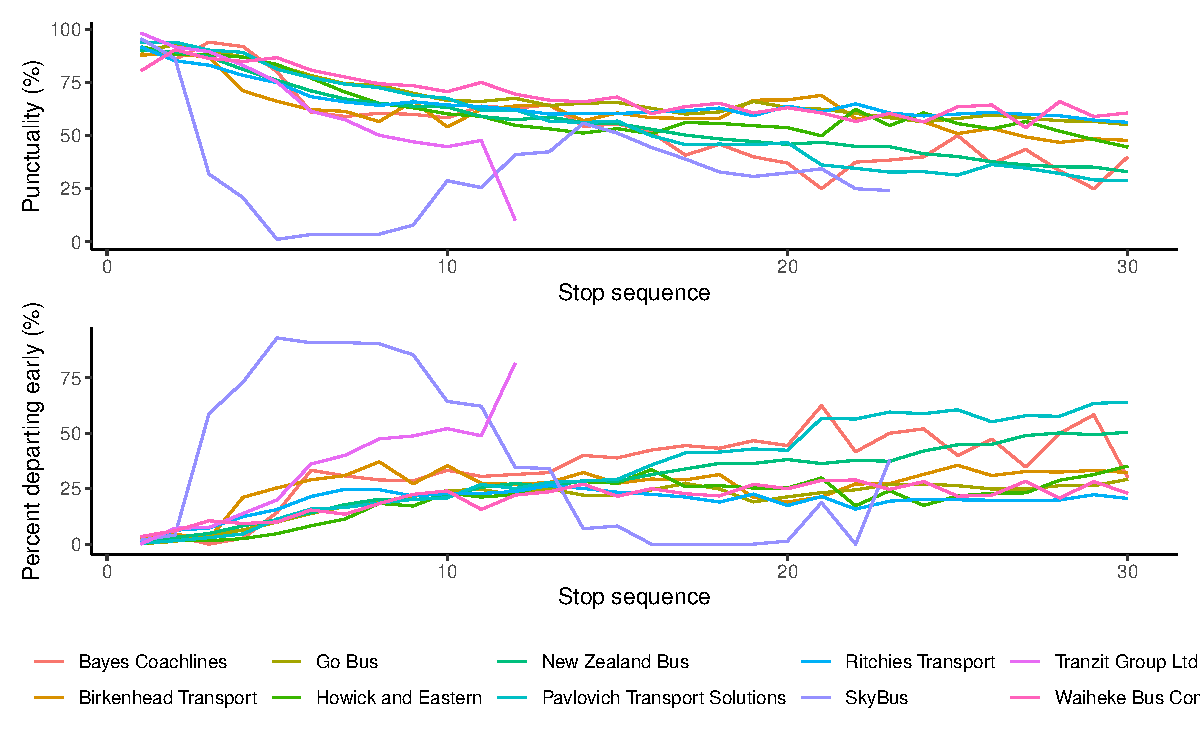
\includegraphics[width=\linewidth]{figure/schedule_adhere-1} \caption[Punctuality of Auckland's transport service providers]{Punctuality (top) and percentage of services arriving early (bottom) for Auckland's transport service providers by stop sequence. Punctuality is measured by the percentage of services departing between 1 minute early and 5 minutes late.}\label{fig:schedule_adhere}
\end{figure}


\end{knitrout}



Given that many of the issues with Auckland's transport system relate to infrastructure, the simplest solution is improved, reliable \gls{rti}. Auckland Transport uses \gls{gtfs}, a specification for how transit data should be organised \citep{GoogleDevelopers_2006}. Part of \gls{gtfs} provides a simple method for predicting arrival times, which is what Auckland Transport and other agencies use. In this method, \emph{trip updates} are reported when a bus arrives or departs from a stop, and includes the vehicle's \emph{delay} (the difference between scheduled and actual arrival). Arrival time at upcoming stops is then estimated by adding this delay to their scheduled arrival times. This method quickly runs into problems if the scheduled travel times are not accurate and drivers do not actively adhere to them.


Besides being inaccurate and unreliable, arrival times based on schedule and current delay are prone to sudden changes in the vehicle's delay. For example, if the bus encounters heavy traffic between stops, it will get later, but this is not reported to passengers until the bus finally arrives at the next stop. When it does, passengers waiting at stops farther along see the \gls{eta} suddenly increase. Another common occurrence is when the bus is delayed on a previous trip: the default arrival time estimate is the scheduled arrival time, so until the bus starts the trip, the \gls{eta} is as scheduled. When the bus is delayed, it may commence the route ten or more minutes late, and when it finally does, the \glspl{eta} at stops suddenly increase by ten (or more) minutes. If the \gls{eta} reaches zero before the bus begins the trip, the bus disappears from the \gls{dms} completely. These scenarios all contribute to traveller frustration and lack of trust in the system.


Conversely, \gls{gtfs} provides an opportunity for a standard, globally available framework: ``The standardised format means that innovative tools and products that utilize GTFS can easily be applied across transit agencies.'' \citep[26]{TCRP_2020}. It is therefore desirable to have a framework that is capable of using solely \gls{gtfs} data to model transit vehicles, estimate traffic conditions throughout the network, and predict arrival times. Location-specific features, such as taxis or intersection locations, should not be required, but could be added as necessary provided the framework is structured to allow it.


The components described in the literature as essential to arrival time prediction are travel time and dwell time. To the best of our knowledge, there is no system based solely on \gls{gtfs} data that provides a means of combining data across routes to estimate traffic conditions and use them to improve arrival time prediction.



\section{Research outline}
\label{sec:proposal}

Public transport is essential wherever people need to get to and from work, school, or other activities dependably. However, in this age of cellphones and \gls{rti}, travellers have come to expect, at the very least, a reliable countdown on the \gls{dms} at their stop. In Auckland, this is not the case. The unreliability of \glspl{eta} makes them unusable for real-time journey planning, causing difficulties for commuters who rely on public transport and potentially driving them to consider alternative---often private---transport options.


The central focus of this thesis is to develop an arrival time prediction application that accounts for real-time traffic information obtained from both static and real-time data provided by \gls{gtfs}. This means that the application can be applied to any city using \gls{gtfs}, and not solely Auckland, as many of the problems discussed will be present elsewhere. We explore how traffic state can be estimated independently of routes so that routes that use the same roads can share travel time or speed information. Our goal is to make arrival time predictions which, by accounting for real-time traffic conditions, are more reliable than those currently available in Auckland. However, it is clear from both the literature and personal experience that substantial levels of uncertainty are inescapable in transit prediction. For this reason, we focus on capturing the uncertainty in the model and estimating the \emph{arrival time distribution}, which can be summarized using, for example, prediction intervals.


We also consider journey planning, notably the use of arrival time distributions to make decisions, since Auckland (and other) transit providers offer no such service. Auckland Transport's ``journey planning'' is based solely on the scheduled timetables, as do transit directions provided by Google Maps\footnote{\url{https://maps.google.com}}. \Citet{Berczi_2017} demonstrate the use of probabilistic arrival time distributions in a real-time dynamic routing problem. It is not our intention to solve the routing problem (selecting candidate routes from origin to destination), but instead to demonstrate the reliability (or usefulness) of our arrival time distribution in choosing between alternative routes. This could then be incorporated into a dynamic routing framework that uses the probabilities of events to make decisions.


Before approaching this problem, I first provide an overview of the relevant background information in \cref{cha:data}. This includes an overview of \gls{gtfs} and a discussion of the characteristics of real-time transit data. We will also examine how a \emph{network} can be constructed from \gls{gtfs} data to allow the sharing of information across independent routes. Lastly, I give a brief introduction to \emph{recursive Bayesian filtering}, an approach to modelling data in real-time that is used extensively throughout this thesis.


Having laid some foundations, we begin the process of real-time prediction by first modelling the state of a transit vehicle, which is updated whenever new data is received. One important aspect of \cref{cha:vehicle_model} involves removing all unnecessary uncertainty. \Citet{Cathey_2003} (and others) used \emph{map-matching} to calculate the vehicle's trip-distance-travelled from the reported \gls{gps} coordinates. As part of the vehicle model, I propose a method of removing this step and incorporating \gls{gps} observations directly into the likelihood function to overcome several of the issues identified in \cref{cha:data}. The main goal of \cref{cha:vehicle_model} is to use real-time transit vehicle observations to estimate vehicle speed along roads. This is similar to the work of \citet{Celan_2017,Celan_2018} who used historical data to estimate average vehicle speed along roads in a \emph{network}.


After observing the speeds of transit vehicles travelling around Auckland, we can model the real-time \emph{traffic state} of the road network. Similar to the work of \citet{Shalaby_2004} we develop a \kf{} that allows real-time estimation of network state in \cref{cha:network_model}. A large part of this consists of estimating the necessary model parameters from historical data and assessing the real-time accuracy of our model. As many previous researchers have noted, predicting future travel times (which depend on road state) is difficult and requires a more complex model than the \kf{}. At the end of \cref{cha:network_model} I discuss a possible approach to forecasting that could later be incorporated into the arrival time prediction component of our application.


Finally, we come to arrival time estimation itself, which combines vehicle and road states to obtain an arrival time distribution. In \cref{cha:prediction}, I demonstrate how the distribution itself is computed and compare our approach to several others. Then, in \cref{cha:etas}, I derive a simplified arrival time \gls{cdf} and present several forms of summary statistics that could be displayed to commuters (point and interval estimates).  We also explore the use of the \gls{cdf} to answer journey planning questions concerning, for example, journey length or the probability of on-time arrival. These results focus on the reliability and potential usefulness of our method's predictions compared to those currently available in Auckland.


Since this is a real-time application, we assess its computational performance throughout. Therefore, at the end of each chapter, I describe the programmatic considerations of the application and discuss the relative components of the \Rstats{} package \pkg{transitr} developed as part of this research. The target for real-time predictions---from the time the data is first requested from the server until \glspl{eta} are available for travellers---is 30~seconds.


Finally, in \cref{cha:discussion}, we review our methods and findings and comment on what could be done to improve our application in the future. The role of \gls{rti} in public transport is only going to become more critical as cities---particularly Auckland---grow. Improving the reliability of the information is the first step to increasing ridership.

\chapter{\Rt{} transit data}
\label{cha:data}



\AT{} operates a fleet of vehicles consisting of buses, trains, and ferries to transport passengers around Auckland, New Zealand's most populous urban region \citep{StatsNZ_2019}, from Wellsford in the north to Pukekohe in the south. Serving the region are 1040~routes,\footnote{As of 12 August 2019, sourced from \url{https://at.govt.nz/}.} each providing a service from an \emph{origin} to a \emph{destination} via a specified sequence of \emph{stops} at which passengers may board or alight.


For each route, one or more \emph{trips} are scheduled to operate, typically departing from the origin stop at a fixed time, with approximate arrival times for the intermediate stops along the way. In some cases, services wait at specific stops until the scheduled departure time, known as a \emph{layover}; in others, drivers may adjust their speed to adhere to the schedule. In most cases, however, drivers do not heed the schedule and drive along the route at whatever speed is reasonable.\footnote{This is what I have observed over 10~years of catching public transport, but also refer back to \cref{fig:schedule_adhere}.} Not all trips run every day; typically trips are scheduled as `weekday', `Saturday', or `Sunday and public holidays'. Altogether there are (at the time of writing) 24,919~trips provided by \AT{}, 14,022 of which run every weekday.


The assignment of routes, trips, and stops is a common occurrence in transport systems, to the extent that it was formalised by Google's \emph{\acrfull{gtfs}} \citep {GoogleDevelopers_2006}. \GTFS{} provides detailed guidelines of how transit data should be organised, making it significantly easier for external systems to access, with the primary example being Google Maps. However, plenty of other applications exist that make use of it.\footnote{Including the one we are presenting.} \GTFS{} has now been adopted by 1,234~providers across 672~locations globally which are shown in \cref{fig:gtfs_feeds}. \Cref{sec:gtfs} provides further information on \gls{gtfs}.

\begin{figure}
\centering
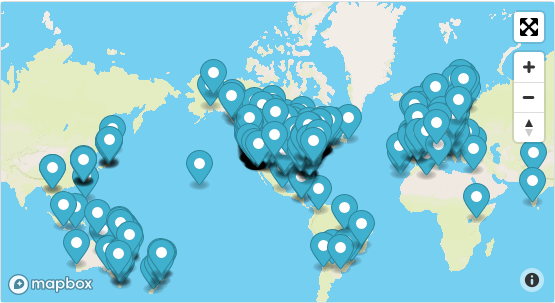
\includegraphics[width=0.8\textwidth]{figure/gtfs_feeds.png}
\caption[Locations of GTFS feed providers]{Locations of the 672~\GTFS{} feed providers,\\
sourced from \url{http://transitfeeds.com/} on 12 Feb 2020.}
\label{fig:gtfs_feeds}
\end{figure}


The vehicles servicing the trips are observed as they travel along the route, either as intermittent \GPS{} locations (\emph{vehicle positions}), or on arrival at or departure from bus stops along the way (\emph{trip updates}). The structure of this data is specified by `GTFS-realtime',\footnote{\url{https://developers.google.com/transit/gtfs-realtime}} and is described in detail in \cref{sec:realtime-data}, along with a discussion of the issues encountered using the \AT{} data.


One of the main ideas we discussed in \cref{sec:literature} was the importance of combining data from multiple routes when predicting arrival times. As it stands, there is no direct method for determining if two routes overlap---that is, share a common path---from \GTFS{} data. The most straightforward approach is to compare subsequences of stops, with routes servicing the same stops most likely following the same path between them. There are, however, several situations where this is not the case. We formalise this idea, as well as expand on it, in \cref{sec:route-segments}.


The real-time nature of the application demands that predictions are made as soon after observing the data as possible. For this reason, \glspl{rbm} are a logical choice for estimating states in real-time and have been used extensively in the literature. This family of models are commonly used in vehicle tracking applications \citep{Zhao_1997,Mutambara_2000,Carpenter_1999,Wall_1999}, allowing the vehicle's state (such as speed) to be estimated from a real-time sequence of noisy measurements of its location. The final section of this chapter provides an introduction to the \glspl{rbm} used throughout the remainder of this thesis.


\section{GTFS}
\label{sec:gtfs}

\glsresetall\phantom{\gls{gps}}

The adoption of GTFS \citep{GoogleDevelopers_2006} by public transport agencies around the world has made it possible for applications such as Google Maps to access and display public transport data to users, regardless of their location. The main goal of GTFS is to specify, in detail, how transit data should be organised so that it is consistent across agencies around the world. As a result, it does not matter whether you are in Auckland, Paris, or C\'ordoba; Google Maps can show you public transport directions by accessing local \gls{gtfs} data.


\GTFS{} consists of two components, \emph{static} and \emph{real-time}.\footnote{The official name is `GTFS-realtime'.} The static component specifies how information about the schedule, fares, and route geographies are organised, while the \emph{real-time} component specifies the format for real-time data: vehicle locations, stop updates and \glspl{eta}, and service advisories. Each of the static and real-time components is implemented by the transit provider; for example, \AT{}'s \GTFS{} service is hosted at \mbox{\url{https://dev-portal.at.govt.nz}}.


\subsection{Static GTFS}
\label{sec:gtfs_static}


\begin{table}[t]
\centering
\fontsize{10}{12}\selectfont
\begin{tabular}{ll}
\toprule
Term & Definition \\
\midrule
route & a collection of \emph{trips} that are displayed to comuters
as a single service \\
trip & a journey servicing two or more stops at a specific time \\
stop & a location where passengers are picked up or dropped off \\
stop time & the (scheduled) times at which vehicles
will arrive at stops for each trip \\
shape & the GPS track a vehicle will take for a specific route \\
\bottomrule
\end{tabular}
\caption[Definitions of GTFS terms]{Definitions of the relevant GTFS terms from \url{https://developers.google.com/transit/gtfs/reference/}}
\label{tab:gtfs_terms}
\end{table}


There are several components of GTFS that are of particular interest to us: routes, trips, stops, stop times, and shapes. The definitions of these terms are given in \cref{tab:gtfs_terms} and \cref{app:gtfs}. Extensive documentation can be found on the GTFS website.\footnote{\url{https://developers.google.com/transit/gtfs/}}


\Cref{fig:gtfs_nw} demonstrates a single \emph{route} along which there are two active \emph{trips} (A and B). The route's \emph{shape} is represented by the line connecting the six \emph{stops} numbered 1--6. The real-time arrivals board or \gls{dms} is shown for stop~5, displaying the scheduled \emph{stop time} (arrival time) for each trip at that stop. The additional information displayed is described in the next section.



\begin{knitrout}\small
\definecolor{shadecolor}{rgb}{0.969, 0.969, 0.969}\color{fgcolor}\begin{figure}

{\centering 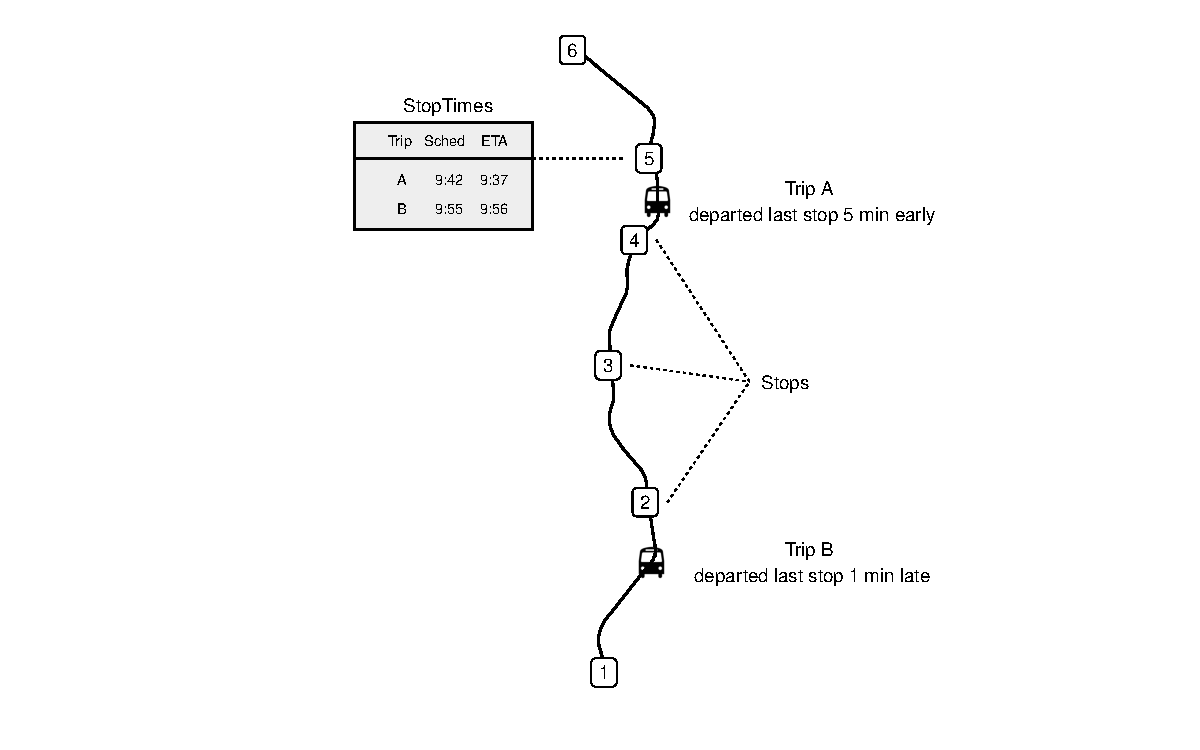
\includegraphics[width=\textwidth]{figure/gtfs_nw-1} 

}

\caption[The main components of a GTFS feed]{The main components of a GTFS feed for a single \emph{route} with two \emph{trips} (A and B) travelling along a \emph{shape} path. The numbered squares represent \emph{stops}, and the scheduled arrival times of each trip at stop 5 are displayed in the \emph{stop times} box.}\label{fig:gtfs_nw}
\end{figure}


\end{knitrout}



Transport providers typically distribute static \GTFS{} data in plain text files, one for each of the components (such as \verb+routes.csv+ and \verb+trips.csv+). Often these are available to download as a single ZIP archive, so the data is easily loaded into a \emph{relational database}, which is described further in \cref{app:gtfs}. The \Rstats{} package developed as part of this work provides the \verb+create_gtfs()+ function to do this automatically:
\begin{knitrout}\small
\definecolor{shadecolor}{rgb}{1, 1, 1}\color{fgcolor}\begin{kframe}
\begin{alltt}
\hlkwd{library}\hlstd{(transitr)}
\hlstd{nw} \hlkwb{<-} \hlkwd{create_gtfs}\hlstd{(}\hlstr{"at_gtfs.zip"}\hlstd{,} \hlkwc{db} \hlstd{=} \hlstr{"at_gtfs.sqlite"}\hlstd{)}
\end{alltt}
\end{kframe}
\end{knitrout}


Within these separate files or tables, the data is stored as per \GTFS{}. Importantly, shapes are stored as sequences of coordinates that draw a path on a map, while stops are represented as a single coordinate marking the location of the bus stop. Stop times are stored in trip-stop pairs with one row for every stop of each trip, along with the scheduled arrival and departure times.\footnote{There are 732,184 rows in the stop times table for Auckland Transport!}



On its own, the static \GTFS{} information can be used like a printed timetable, allowing simple journey planning to take place. As such, it provides a ``fallback'' state in situations where no \rt{} information is available for a given trip: scheduled stop times can be thought of as \emph{prior information}, a core component of the Bayesian paradigm.



\subsection{Real-time GTFS}
\label{sec:gtfs_rt}

The real-time component of \GTFS{} is responsible for handling vehicle positions, trip updates (arrivals at and departures from stops), and service alerts (cancellations and stop closures, for example). Data is processed by a central server and then stored appropriately to enable quick access via \glspl{api}. There is, therefore, the additional need of a server that can handle vast numbers of \gls{api} requests. As such, only a subset of transport providers using \GTFS{} have also implemented the real-time component. Below we give a summary of these components, but further information is available on the \GTFS{} website.\footnote{See \url{https://developers.google.com/transit/gtfs-realtime/}.}


\subsubsection{Vehicle positions}
\label{sec:gtfs_rt_vehicle}

There are several key components to a vehicle position (in the context of \GTFS{}). The \emph{vehicle descriptor} includes information about the physical vehicle, while a \emph{trip descriptor} holds information about the trip being serviced. A \emph{timestamp} specifies exactly when the observation was made, and a \emph{position} contains the actual data, such as the \gls{gps} observation, as is demonstrated by the bus images in \cref{fig:gtfs_nw}.


The specification also allows for additional measurements, such as \emph{speed} or an \emph{odometer} reading. However, these were not available from \AT{} at the time this work was carried out, so they are not included in our application. It is well worth noting, however, that they could be integrated with minimal effort if they become available.


\subsubsection{Trip updates}
\label{sec:gtfs_rt_trip}

As vehicles equipped with \gls{avl} technology arrive at and depart from stops, information about their times of arrival and, most importantly, \emph{schedule adherence} is stored in trip updates. These also contain a \emph{trip descriptor}, as well as one or more \emph{stop time updates}. GTFS-realtime allows storing of stop time updates for all previously visited stops, as well as predictions for upcoming stops. However, Auckland Transport only stores the most recent update.


Each stop time update reports either the arrival or departure time and, where schedule information is available, the schedule adherence by way of an \emph{arrival} or \emph{departure delay} (in seconds). \Cref{fig:gtfs_nw} displays this information offset to the right of each bus location. The on-board \gls{avl} device is responsible for detecting these events, and they are not necessarily linked to the \gls{gps} position of the vehicle. In Auckland, each trip update also triggers a vehicle location update, but the coordinates are those of the \emph{stop}, not of the vehicle. This leads to some of the problems addressed in \cref{sec:realtime-data}.


In Auckland, the current delay is added to the scheduled arrival time, as shown on the \gls{dms} in \cref{fig:gtfs_nw}. We will certainly be discussing the issues associated with this method shortly, and indeed be making comparisons to it throughout the thesis.



\subsubsection{Service alerts}
\label{sec:gtfs_rt_alerts}

Less important for the current work, but essential for reliable \gls{rti}, \emph{service alerts} enable transit operators to modify the static \GTFS{} in real-time. So, when a trip is cancelled, they can send out a service alert announcing the cancellation,\footnote{Although they often don't.} which is then displayed to passengers as a ``C'' on the \gls{dms}. It is also possible to add trips, for example during special events, or to reroute trips around stop closures, but this is beyond the scope of our work.



\subsection{Accessing \rt{} data (API)}
\label{sec:gtfs_rt_api}

Distributing vehicle locations, trip updates, and service alerts to passengers quickly and usefully requires more than just a \gls{dms} at bus stops. Personal mobile devices have revolutionised the way we live our lives, and developers are continually creating new applications to assist with everyday activities. Included in these are transit applications, which are capable of conveying real-time \GTFS{} data to passengers.


The most common method of distributing real-time data is via an \gls{api}. This is, in simple terms, a fixed web address from which developers can request a data file---either \prog{JSON} or, in the case of some \GTFS{} systems, \prog{protobuf}\footnote{See \url{https://developers.google.com/protocol-buffers}}---which can then be parsed and displayed to users. Usually, developers need to register for an \emph{\gls{api} key} which helps to control server demand by limiting the number of requests a user can make, or control access to specific data. The \pkg{transitr} package includes the ability to connect to a \GTFS{}-based \gls{api} easily:
\begin{knitrout}\small
\definecolor{shadecolor}{rgb}{1, 1, 1}\color{fgcolor}\begin{kframe}
\begin{alltt}
\hlstd{url} \hlkwb{<-} \hlstr{"https://api.at.govt.nz/v2/public/realtime/vehiclelocations"}
\hlstd{nw} \hlkwb{<-} \hlkwd{load_gtfs}\hlstd{(}\hlstr{"at_gtfs.sqlite"}\hlstd{)} \hlopt
    \hlkwd{realtime_feed}\hlstd{(url)} \hlopt
    \hlkwd{with_headers}\hlstd{(}
        \hlcom{# this varies by provider}
        \hlstr{"Ocp-Apim-Subscription-Key"} \hlstd{=} \hlkwd{Sys.getenv}\hlstd{(}\hlstr{'APIKEY'}\hlstd{)}
    \hlstd{)}
\end{alltt}
\end{kframe}
\end{knitrout}

\section{Charactersitics of real-time transit data}
\label{sec:realtime-data}

There are a range of \gls{avl} technologies which allow transit vehicles to report their locations in real-time. The most common of these is now the \gls{gps}, which provides the longitude and latitude of the vehicle. In the simplest of deployments, each vehicle reports its location to a central server at a fixed time interval. The server then collates the reports from all buses in the fleet and makes them available via an \gls{api}.


Another type of real-time data available to us is arrival and departure information at bus stops. When a vehicle arrives at or departs from a stop,\footnote{Or thinks it does, see \cref{sec:vp_data}.} it reports to the server which stop it is at along with its time of arrival or departure. The server then computes the delay (the time between actual and scheduled arrival or departure), collates the data from multiple vehicles, and also makes these available through an \gls{api}.


\Gls{rti} can be displayed in one of two ways. \Gls{gps} positions are displayed on a map accessed through a mobile app, allowing commuters to see where their bus was when it last reported its location. For trip updates, the \emph{current delay} is added to the scheduled arrival time and displayed to commuters, usually as a \emph{time until arrival}, in minutes.\footnote{That is ``scheduled arrival time + delay - current time''.} The \gls{eta} can be displayed either on a mobile app or, more commonly, on a \gls{dms} at the stop.


What we have just described is, in fact, the entirety of \gls{rti} in Auckland and some other transit locations around the world. While at first it seems an adequate solution, discussion with just about any regular public transport user suggests otherwise. The reasons for this become apparent with a little scrutiny, which we will now uncover.


\subsection{Vehicle positions}
\label{sec:vp_data}

Every measurement of a data point comes with some associated error. In the case of \gls{gps} devices, this error is usually small with precision depending on the quality of the device. However, any device can succumb to several factors which may place the bus far from its expected path, the primary reason being buildings or other obstacles resulting in a poor signal \citep{Xinghao_2013,Mutambara_2000,Zhao_1997}. Surprisingly, however, this is not the main issue with vehicle position data.


Object tracking has been well studied, and many algorithms exist for tracking an object through space using \gls{gps} observations. However, these usually take high-frequency observations (\citet{Gustafsson_2002} updated the car's location twice per second) which can generate an almost exact real-time estimate of the object's actual position.


Many examples of real-time object tracking exist, but the most relatable to most readers will be in their pocket. When getting directions from your phone, the maps application requests the user's phone's location continuously, providing the exact location with a second or less of delay. However, have you ever been driving along, following directions, and accidentally missed the turn-off? Often, the maps application will show you as \emph{on course} for several seconds until it realises that you have well and truly gone off-track and reroutes you. This is an example of a real-time position tracking algorithm that is attempting to follow the device's location while simultaneously accounting for inherent noise in the measurements. When the driver first goes off track, the algorithm assumes this is a measurement error and assumes the vehicle is on course. Eventually, the error becomes large and consistent enough that the model stops assuming the driver is following the planned route.


With real-time transit data, the frequency of observations is vastly reduced, with observations obtained with anything from ten seconds to a minute (or more) between them. This makes it very difficult to estimate the vehicle's exact location. On receiving a vehicle position that seems incorrect, we must wait until we receive the next observation to determine if it was the result of a bad measurement or a real event.


Another major complication with the Auckland Transport vehicle data is that vehicles often report their location when arriving at or departing from a bus stop. However, instead of reporting their \gls{gps} location as measured from the \gls{gps} device, they report the location of the bus stop itself, which is known exactly. So, what happens when the bus approaches a bus stop at speed, only to come to a halt at an intersection 100~m before hand? The vehicle's \gls{avl} system continues predicting the trajectory and places the vehicle at the bus stop before it actually arrives. This triggers a trip update (section~\ref{sec:tu_data}), which itself produces a vehicle position update \emph{at the bus stop}. However, a passenger standing at the stop will see the bus sitting at the lights even though the \gls{dms} displays the bus as having arrived. For the passenger waiting at this stop, this is of no concern, as they can see the bus and have no need for real-time data. For passengers farther down the line, however, this can have some frustrating implications.

Another related phenomenon exists in which the bus may appear to go backwards according to the sequence of \gps{} coordinates, discussed in detail in \cref{sec:data_issues}. The main consequence of this problem is that within the data processing component of our application, we check for vehicle position updates associated with trip updates and remove them (that is, we use the trip update and not the vehicle position).\footnote{This seems straightforward, but was frustrating until identified.}




\subsection{Trip updates}
\label{sec:tu_data}

As alluded to earlier, trip updates are prone to measurement error. Without human intervention, it is challenging for the \gls{gps} tracking system on the bus to determine exactly when the bus arrives at or leaves a bus stop. In situations like the one described above, the arrival time may be reported before the bus arrives, resulting in a premature arrival time and, more importantly, \emph{a reduced delay}. Traffic lights may hold up a bus for a minute (or more), so the bus may, for argument sake, appear to arrive precisely on time with a delay of zero minutes. The result of this is the propagation of the current delay to all future stops, which then display an \gls{eta} that matches the scheduled arrival time. However, two minutes later, after the bus has finally arrived at the stop, dropped off and picked up passengers, it departs, triggering another trip update. The delay, now two minutes, is propagated to upcoming stops. Passengers waiting at these stops see the \gls{eta} jump suddenly by two minutes, as demonstrated in \cref{fig:tu_eta_jump}, leading inevitably to much frustration for passengers.

\begin{knitrout}\small
\definecolor{shadecolor}{rgb}{0.969, 0.969, 0.969}\color{fgcolor}\begin{figure}

{\centering 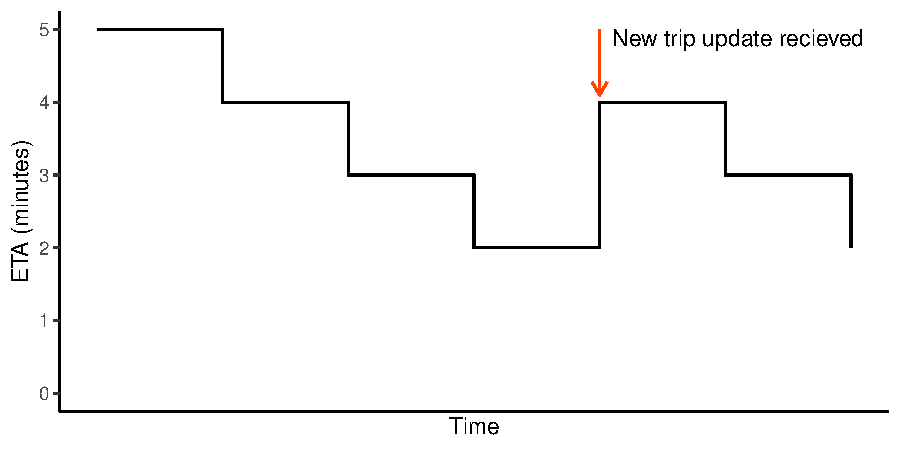
\includegraphics[width=.8\textwidth]{figure/tu_eta_jump-1} 

}

\caption[ETAs as percieved by passengers under the current system]{The current system displays \glspl{eta} to passengers as integer minutes which decrease over time. When new data is recieved (marked by an arrow) the \gls{eta} is updated, which may result in a sudden ``jump'', as demonstrated.}\label{fig:tu_eta_jump}
\end{figure}


\end{knitrout}


The reverse can also occur, for example, if for some reason the bus reports its arrival or departure late. However, more prevalent is that the update is skipped altogether, so a bus that was five minutes behind schedule has made up several minutes and arrives at the bus stop while the \gls{dms} still shows it as being two minutes away. At first, this may seem like a good thing: passengers at the stop have a shorter wait. Other passengers making their timely way to the bus, however, may have to sprint or miss the bus altogether, which is not ideal.


The main repercussion of the described issues is that arrival and departure time data become very noisy and difficult to trust. They do, however, provide a lot of information without which it would be challenging to infer the trajectory of a bus between stops---which is the primary aim of this part of our work. We discuss this further in \cref{sec:pf-likelihood} when I present the likelihood function.



\section{Constructing a network from GTFS data}
\label{sec:route-segments}

In \cref{sec:literature}, I reported how arrival time prediction is greatly improved when data from multiple routes is combined to estimate traffic conditions \citep{Yu_2011}. However, many of these applications were specific to a certain set of routes, or used external information (such as automatic toll readers and taxis) to get \rt{} traffic information. We wanted to develop a \emph{simpler}, \emph{more generalised} approach using solely \GTFS{} data (stops and shapes) to construct a network of non-overlapping\footnote{Except of course reverse directions.} road segments. The network should consist of \emph{nodes} (which could be intersections or bus stops) connected by \emph{edges}, or road segments, which is similar to the structure used by \citet{Celan_2017,Vuurstaek_2018}.


The main goal of the network is to detect where any two routes overlap, even partially. There are several possible approaches to this, but the simplest is to look at common subsequences of bus stops. Of course, stops do not make optimal node locations because routes do not diverge \emph{physically} at stops---that would require locating \emph{intersections}. However, due to difficulties in finding intersections from either the \gls{gtfs} data or outside information, we opted to use bus stops for this work. \Cref{fig:gtfs_route_network} shows a simple route diagram with several overlapping routes. We see that each link between stops is common across routes, but routes that merge at intersections do not merge in the network until they reach a common stop.


\begin{knitrout}\small
\definecolor{shadecolor}{rgb}{1, 1, 1}\color{fgcolor}\begin{figure}

{\centering 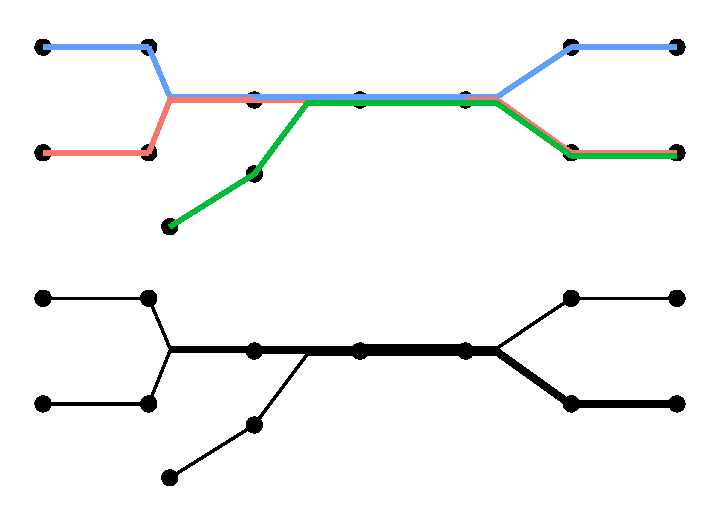
\includegraphics[width=0.6\textwidth]{figure/gtfs_route_network-1} 

}

\caption[Simplified network diagram with road segments constructed from stop sequences]{Simplified network diagram with road segments constructed from stop sequences. Top: routes are coloured individually. Bottom: road segments are sized by the number of associated routes.}\label{fig:gtfs_route_network}
\end{figure}


\end{knitrout}





One other issue with \AT{}'s \GTFS{} data is that all object IDs are \emph{versioned}. That is, instead of a route having an ID of \verb+02702+, the date and version number are appended to it: \verb+02702-20190806160740_v82.21+. This is the same for the IDs of trips, shapes, and stops, making it challenging to transfer existing segments based on stops from previous versions of the \gls{api} and requiring an additional step to remove the version information from the raw data.


The algorithm we implemented uses only bus stops but can extend to intersections, if available. Each stop along a route is assessed to see if any nodes already exist in that location to avoid the versioning issue mentioned above. If so, the route is assigned the existing node; otherwise, a new node is created and assigned instead. Road segments are defined by unique one-way connections between two stops: there can only be one segment going from node $A$ to node $B$ (the reverse is considered a different segment). The network is constructed by the \pkg{transitr} package's \verb+construct()+ function:
\begin{knitrout}\small
\definecolor{shadecolor}{rgb}{1, 1, 1}\color{fgcolor}\begin{kframe}
\begin{alltt}
\hlkwd{library}\hlstd{(transitr)}
\hlstd{nw} \hlkwb{<-} \hlkwd{load_gtfs}\hlstd{(}\hlstr{"at_gtfs.sqlite"}\hlstd{)} \hlopt \hlkwd{construct}\hlstd{()}
\hlstd{transitr}\hlopt{:::}\hlkwd{load_road_segments}\hlstd{(nw)} \hlopt \hlkwd{head}\hlstd{()}
\end{alltt}
\begin{verbatim}
##   road_segment_id node_from node_to    length
## 1               1      5414     537  485.6548
## 2               2       537    3987  196.5567
## 3               3      3987    7265  567.0883
## 4               4      7265    1255 1049.0181
## 5               5      1255    4099  682.5452
## 6               6      4099    3436  535.0515
\end{verbatim}
\end{kframe}
\end{knitrout}

\section{Recursive Bayesian models}
\label{sec:recursive-bayes}

The most challenging problem we face in this application is its \rt{} nature. Vehicle's report their current location, from which we want to estimate road speeds to predict arrival times, all within no more than 30~seconds. Fortunately, a certain class of models suit themselves well to \rt{} applications, and are indeed used in many vehicle tracking and robotics applications \citep{Anderson_1979,Gustafsson_2002,Mutambara_2000}: \glspl{rbm}, sometimes referred to a \emph{sequential Bayesian estimation}.


In a typical analysis, data $\mat{Y}$ would be stored in an $n\times k$ matrix corresponding to $k$ measurements of $n$ variables over time. Then Bayes' rule is used to estimate the posterior distribution of an $m\times k$ matrix of parameters $\mat{X}$ all at once,
\begin{equation}
\label{eq:bayes}
p(\mat{X}\cond{}\mat{Y}) =
\frac{
    p(\mat{X})
    p(\mat{Y}\cond{}\mat{X})
}{
    p(\mat{Y})
},
\end{equation}
using, for example, \agls{mcmc} algorithm. This is usually a computationally intensive procedure and takes much longer than 30~seconds to converge.


In a real-time application, the columns of $\mat{Y}$ are observed sequentially, so that at time $t_k$ we have observed
\begin{equation}
\label{eq:bayes_y_vector}
\mat{Y} = \boldsymbol{y}_{1:k} = [\boldsymbol{y}_1,\cdots,\boldsymbol{y}_k],
\end{equation}
to estimate
\begin{equation}
\label{eq:bayes_x_vector}
\mat{X} = \bx_{0:k} = [\boldsymbol{x}_0,\cdots,\boldsymbol{x}_k],
\end{equation}
where $\boldsymbol{x}_0$ is the \emph{initial state} of the object. Rather than refitting the full model, as would be necessary when using \gls{mcmc}, \gls{rbe} allows us to combine the previous \emph{posterior estimate} of the state with the new information.

\Glspl{rbm} make two general assumptions. The first is that $\boldsymbol{x}$ follows a Markov process such that the state at time $t_k$ depends only upon the state at time $t_{k-1}$:
\begin{equation}
\label{eq:rbe_markov}
p(\boldsymbol{x}_k \cond{} \boldsymbol{x}_{0:k-1}) =
p(\boldsymbol{x}_k \cond{} \boldsymbol{x}_{k-1}).
\end{equation}
The joint distribution of the underlying state parameters is therefore
\begin{equation}
\label{eq:rbe_joint_x}
\begin{split}
p(\bx_{0:k})
&= p(\bx_0)p(\bx_1\cond{}\bx_0)p(\bx_2\cond{}\bx_{0:1})\cdots
p(\bx_{k}\cond{}\bx_{0:k-1}) \\
&= p(\bx_0)p(\bx_1\cond{}\bx_0)p(\bx_2\cond{}\bx_1)\cdots p(\bx_k\cond{}\bx_{k-1}) \\
&= p(\bx_0)\prod_{i=1}^k p(\bx_i\cond{}\bx_{i-1}).
\end{split}
\end{equation}

The second assumption is that the observations $\boldsymbol{y}_k$ of the state depend only on the current state and are independent of one another:
\begin{equation}
\label{eq:rbe_obs}
p(\boldsymbol{y}_k \cond{} \boldsymbol{x}_{0:k}, \boldsymbol{y}_{0:k-1}) =
p(\boldsymbol{y}_k \cond{} \boldsymbol{x}_{k}).
\end{equation}
Thus, the data has joint likelihood
\begin{equation}
\label{eq:rbe_joint_lh}
\begin{split}
p(\boldsymbol{y}_{1:k}\cond{}\bx_{0:k})
&= p(\boldsymbol{y}_1\cond{}\bx_{0:1})\cdots p(\boldsymbol{y}_k\cond{}\bx_{0:k}) \\
&= p(\boldsymbol{y}_1\cond{}\bx_1)\cdots p(\boldsymbol{y}_k\cond{}\bx_k) \\
&= \prod_{i=1}^k p(\boldsymbol{y}_i\cond{}\bx_i)
\end{split}
\end{equation}
and marginal distribution
\begin{equation}
\label{eq:rbe_marginal_y}
p(\boldsymbol{y}_{1:k}) = p(\boldsymbol{y}_1)\cdots p(\boldsymbol{y}_k)
= \prod_{i=1}^k p(\boldsymbol{y}_i).
\end{equation}



We now express the posterior distribution $p(\bx_{0:k}\cond{}\boldsymbol{y}_{1:k})$ using \cref{eq:bayes} along with \cref{eq:rbe_joint_x,eq:rbe_joint_lh,eq:rbe_marginal_y} as
\begin{equation}
\label{eq:rbe_posterior}
\begin{split}
p(\bx_{0:k}\cond{}\boldsymbol{y}_{1:k})
&= \frac{p(\bx_{0:k})p(\boldsymbol{y}_{1:k}\cond{}\bx_{0:k})}{p(\boldsymbol{y}_{1:k})} \\
&= \frac{
    p(\bx_0)\prod_{i=1}^k p(\bx_i) \cdot
    \prod_{i=1}^k p(\boldsymbol{y}_i\cond{}\bx_i)
}{
    \prod_{i=1}^k p(\boldsymbol{y}_i)
} \\
&= p(\bx_0)\prod_{i=1}^k
\frac{
    p(\bx_i) p(\boldsymbol{y}_i\cond{}\bx_i)
}{
    p(\boldsymbol{y}_i)
}.
\end{split}
\end{equation}
However, we can substitute the first $k-1$ terms in \cref{eq:rbe_posterior} to obtain the following recursive representation:
\begin{equation}
\label{eq:rbe_posterior_recursive}
p(\bx_{0:{k}}\cond{}\boldsymbol{y}_{1:k})
= p(\bx_{0:k-1}\cond{}\boldsymbol{y}_{1:k-1})
\frac{
    p(\bx_{k}) p(\boldsymbol{y}_{k}\cond{}\bx_{k})
}{
    p(\boldsymbol{y}_{k})
}.
\end{equation}
Here, the posterior distribution from the previous time step is used as a \emph{prior} for the next, and so it \emph{recursively} (or \emph{sequentially}) updates the state estimate as new data are observed, making \glspl{rbm} ideal for real-time applications.


There are several types of \glspl{rbe} which consist of two main steps: \emph{predict} and \emph{update}. In the prediction step, the algorithm uses a \emph{transition function} $f$ (or matrix $\mat{F}$) to predict the new state based only upon the current state (\cref{eq:rbe_markov}), while the \emph{update} step incorporates the data to adjust the estimate using a \emph{measurement function} $h$ (or matrix $\mat{H}$) describing the relationship between $x$ and $y$ (\cref{eq:rbe_obs}). These can be expressed by the following model equations:
\begin{equation}
\label{eq:rbe_model}
\begin{split}
\bx_k &= f(\bx_{k-1}, \boldsymbol{w}_k) \\
\boldsymbol{y}_k &= h(\bx_k) + \boldsymbol{v}_k
\end{split}.
\end{equation}
The additional parameters $\boldsymbol{w}_k$ and $\boldsymbol{v}_k$ represent \emph{system noise} and \emph{measurement error}, respectively. The choice of $f$, $h$, and the distributions for the error terms depends on the choice of model. We now discuss two types of \gls{rbe} used throughout this thesis: the \kf{} and the \pf{}.


\subsection{\kf{}}
\label{sec:kf}

Commonly used in vehicle tracking applications, the \kf{} is a very fast, simple estimation method \citep{Anderson_1979} that assumes Gaussian errors and represents the state using a multivariate Normal random variable with length $m$ mean vector and $m\times x$ covariance matrix
\begin{equation}
\label{eq:kf_estimators}
\hat\bx_{k|k} = \E{\bx_k | \boldsymbol{y}_{1:k}}
\quad\text{and}\quad
\mat{P}_{k|k} = \Var{\bx_k | \boldsymbol{y}_{1:k}},
\end{equation}
respectively. A \kf{} implementation requires an $m\times m$ \emph{transition matrix}, $\mat{F}_k$, which defines the relationship between states at time $t_{k-1}$ and $t_k$, and an $n\times m$ \emph{measurement matrix}, $\mat{H}_k$, defining the relationship between $\boldsymbol{y}$, a length $n$ vector, and $\bx$, a length $m$ vector.


The \kf{} version of the model presented in \cref{eq:rbe_model} is
\begin{equation}
\label{eq:kf_model}
\begin{split}
\bx_k &= \mat{F}_k\bx_{k-1} + \boldsymbol{w}_k \\
\boldsymbol{y}_k &= \mat{H}_k\bx_k + \boldsymbol{v}_k
\end{split},
\end{equation}
where $\boldsymbol{w}_k$ and $\boldsymbol{v}_k$ are Normal random variables with mean zero and covariance matrices $\mat{Q}_k$ and $\mat{R}_k$, respectively. The $m\times m$ covariance matrix $\mat{Q}_k$ represents the system noise at time $t_k$, which is defined as the rate of change of the variance of process noise \citep{Cathey_2003}. Measurement error is expressed by the $n\times n$ covariance matrix $\mat{R}_k$.

The \kf{} is implemented through two sets of equations. First is the prediction step, in which the current state (represented by the mean vector and covariance matrix) is predicted based solely on the previous state:
\begin{equation}
\label{eq:ch2:kf_predict}
\begin{split}
\hat\bx_{k|k-1} = \E{\bx_k | \bx_{k-1}}
    &= \mat{F}_k \hat\bx_{k-1|k-1} \\
\mat{P}_{k|k-1} = \Var{\bx_k | \bx_{k-1}}
    &= \mat{F}_k \mat{P}_{k-1|k-1} \mat{F}_k^\top + \mat{Q}_k
\end{split}
\end{equation}
Next, the update step uses the observation $\boldsymbol{y}_k$ to adjust the predicted state using the following set of equations, which are effectively taking a ratio of the state and measurement uncertainties:
\begin{equation}
\label{eq:ch2:kf_update}
\begin{split}
\bz_k &= \boldsymbol{y}_k - \mat{H}_k \hat\bx_{k|k-1} \\
\mat{S}_k &= \mat{R}_k + \mat{H}_k \mat{P}_{k|k-1} \mat{H}_k^\top \\
\mat{K}_k &= \mat{P}_{k|k-1} \mat{H}_k^\top \mat{S}_k^{-1} \\
\hat\bx_{k|k} &= \hat\bx_{k|k-1} + \mat{K}_k \bz_k \\
\mat{P}_{k|k} &= (\mat{I} - \mat{K}_k \mat{H}_k) \mat{P}_{k|k-1}
    (\mat{I} - \mat{K}_k \mat{H}_k)^\top + \mat{K}_k \mat{R}_k \mat{K}_k^\top.
\end{split}
\end{equation}


The simplicity of the \kf{} means that, so long as the number of parameters $m$ is small, states can be estimated quickly with minimal processing demand. This simplicity, together with the fact that it provides an exact solution for the multivariate Normal state space model \citep{Anderson_1979}, makes the \kf{} a strong contender for real-time applications. However, it also makes several strong assumptions about the shape of the parameter distributions and is limited to linear relationships between states and measurements since these must be expressed in matrix form.



\subsection{Particle filter}
\label{sec:pf}

Another framework we use is the \pf{}, a more generalised, numerical approach to recursive Bayesian modelling \citep{Gordon_1993}. The state is approximated by a sample of $\Np$ particles, each of which is an independent point estimate of the state, $\bx\vi_k$, with a weight $w\vi \geq 0$ and $\sum_i w\vi = 1$. The state estimate is expressed using the Dirac delta measure $\dirac$ (see \cref{app:dirac-delta-measure} for details), such that
\begin{equation}
\label{eq:pf_state}
p(\bx_{k-1} | \boldsymbol{y}_{1:k-1}) \approx
\sum_{i=1}^\Np w\vi_{k-1} \DiracMeasure{\bx\vi_{k-1}}{\bx_{k-1}}.
\end{equation}

One advantage of the \pf{} is that we are no longer constrained in the choice of transition function, $f$, or the error distribution. Instead of working with the mean and variance of the state (as is the case with the \kf{}) we work with \emph{independent point estimates} which each represent a plausible state. In \cref{cha:vehicle_model} I use a Normal random variable for system noise, but this could be any appropriate distribution (for example a Cauchy if heavier tails are necessary). The state prediction step is carried out independently on each particle,
\begin{equation}
\label{eq:ch2:pf_predict_particle}
\bx\vi_k = f\left(\bx\vi_{k-1}, \boldsymbol{v}\vi_k\right),
\quad
\boldsymbol{v}\vi_k \sim \Normal{\boldsymbol{0}}{\mat{Q}_k}.
\end{equation}
The prior-predictive distribution of the state, using the Dirac delta measure, is given by
\begin{equation}
\label{eq:ch2:pf_predict_state}
p(\bx_k | \bx_{k-1}) \approx
\sum_{i=1}^\Np w\vi_{k-1} \DiracMeasure{\bx\vi_k}{\bx_k}.
\end{equation}


Next, the state is updated to account for the observation using the likelihood function directly. The particles are reweighted and normalised,
\begin{equation}
\label{eq:pf_reweight}
w\vi_k =
\frac{
    w\vi_{k-1} p(\boldsymbol{y}_k | \bx\vi_k)
}{
    \sum_{j=1}^\Np w\vi_{k-1} p(\boldsymbol{y}_k | \bx\vi[j]_k)
},
\end{equation}
which yields the final posterior distribution of the state,
\begin{equation}
\label{eq:pf_state_post}
p(\bx_{k} | \boldsymbol{y}_{1:k}) \approx
\sum_{i=1}^\Np w\vi_{k} \DiracMeasure{\bx\vi_{k}}{\bx_{k}}.
\end{equation}


Over time, many of the particle weights will go to zero as they disperse due to the system noise \citep{Doucet_2000}. This leaves only a few particles contributing to the state, which, if none end near the actual vehicle location, will result in all vehicles having likelihoods close to zero. To prevent this situation of particle filter \emph{degeneration}, we perform \emph{importance resampling} (a weighted bootstrap) in which particles are sampled, with replacement, according to their weight. Afterwards, particle weights are reset to $N^{-1}$.

\citet{Doucet_2000} describe the use of the \emph{effective sample size},
\begin{equation}
    \label{eq:Neff}
    N_{\text{eff}} \approx \frac{1}{\sum_{i=1}^N (w_k\vi)^2},
\end{equation}
which provides an estimate of how varied the particles are: if too few particles contain most of the weight, resampling should occur. This is similar to the Metropolis-Hasting's proposal and acceptance steps: we propose a sample of state estimates and reject those that are not plausible given the data. If the system noise (proposal distribution) is small, then more particles will be ``accepted'', but we may not propose sufficient trajectories. Conversely, if the noise is too large, then there will be many ``rejections'', reducing the variety of particles (small $N_\text{eff}$).

Another advantage of the \pf{} is its generality. As we discuss in \cref{sec:vehicle_model}, we can easily construct a transition function to describe a complex system, as well as define a likelihood function that accurately represents the relationship between observed and unobserved states.

The main disadvantage is, of course, that the computational demand is high, as each particle is transitioned independently, and resampling can be slow for large $\Np$, having order $\mathcal{O}(\Np\log\Np)$ in the \prog{C++} algorithm we use. However, as we discuss in the next chapter, the advantages far outweigh the additional computational demands of the \pf{}, which can be minimised if implemented carefully.




\section{\Rt{} implementation in Rcpp}
\label{sec:rt-implementation}

In \cref{sec:gtfs} I introduced the \Rstats{} package \pkg{transitr}, which loads a \GTFS{} database and connects to a real-time \gls{api}. The advantage of \Rstats{} \citep{rcore} is its superior ability for processing data of various forms through additional packages, and provision an easy-to-use interface for users. However, when it comes to computational efficiency, \Cpp{} is the better choice. Fortunately, \Rstats{} offers an interface to \Cpp{} through the \pkg{Rcpp} package developed by \citet{Rcpp}. This gives us the speed and memory management capabilities of \Cpp{} from within \Rstats{}.

The general structure of our program has two parts. The first handles data collection from a transit provider and creation of the transit network (\cref{sec:route-segments}), all stored in an \prog{SQLite} database.\footnote{\url{https://www.sqlite.org/index.html}} Users can connect to a GTFS-realtime \gls{api}, as well as pass additional arguments to the generated \obj{gtfs} object, which are then forwarded onto the second part which runs purely within \Cpp{}.

Within the \Cpp{} component, there are two main phases: setup and modelling. During the setup phase, the GTFS database is loaded, and parameter values are established. A vector of \class{Vehicle} objects is initialized to contain the real-time vehicle states. The modelling phase consists of a single \verb+while+ loop which runs until the operating system sends the program a kill signal. It is inside this loop that all of the real-time modelling discussed throughout the remainder of this thesis occurs.

Within the program, we use \gls{oop} to represent objects---both static (routes and trips) and \rt{} (vehicles, road segments). These objects contain a lot of \emph{interdependence}; for example, a trip belongs to a route and vehicles services trips. Pointers are used in \Cpp{} to allow easy access to these relationships without any duplication of information. For example, the route number for a vehicle can be obtained as follows:
\begin{knitrout}\small
\definecolor{shadecolor}{rgb}{1, 1, 1}\color{fgcolor}\begin{kframe}
\noindent
\ttfamily
\hlstd{vehicle}\hlopt{.}\hlstd{}\hlkwd{trip\ }\hlstd{}\hlopt{(){-}$>$}\hlstd{}\hlkwd{route\ }\hlstd{}\hlopt{(){-}$>$}\hlstd{}\hlkwd{route\textunderscore short\textunderscore name\ }\hlstd{}\hlopt{();}\hlstd{}\hspace*{\fill}
\mbox{}
\normalfont
\end{kframe}
\end{knitrout}
As pointers are not fixed, the above example works even after the vehicle changes to another trip. In addition to retrieving information, pointers can be used to pass information between objects. Later in this thesis, vehicles are used to estimate traffic conditions along individual roads, and then forward these observations on to the appropriate road segment. First, note that a route follows a sequence of road segments, which are stored in \Cpp{} using a \verb+std::vector+ containing an ordered sequence of \class{RouteSegment} objects, each pointing to the appropriate \class{Segment}. Thus, once a vehicle completes travel along the segment with index \verb+si+, the observed average speed can be passed directly to the \class{Segment}:
\begin{knitrout}\small
\definecolor{shadecolor}{rgb}{1, 1, 1}\color{fgcolor}\begin{kframe}
\noindent
\ttfamily
\hlstd{vehicle}\hlopt{.}\hlstd{}\hlkwd{trip\ }\hlstd{}\hlopt{(){-}$>$}\hlstd{}\hlkwd{route\ }\hlstd{}\hlopt{()}\hspace*{\fill}\\
\hlstd{}\hlstd{\ \ \ \ }\hlstd{}\hlopt{{-}$>$}\hlstd{}\hlkwd{segments\ }\hlstd{}\hlopt{().}\hlstd{}\hlkwd{at\ }\hlstd{}\hlopt{(}\hlstd{si}\hlopt{){-}$>$}\hlstd{}\hlkwd{segment\ }\hlstd{}\hlopt{()}\hspace*{\fill}\\
\hlstd{}\hlstd{\ \ \ \ }\hlstd{}\hlopt{{-}$>$}\hlstd{}\hlkwd{push\textunderscore data\ }\hlstd{}\hlopt{(}\hlstd{speed}\hlopt{,\ }\hlstd{uncertainty}\hlopt{);}\hlstd{}\hspace*{\fill}
\mbox{}
\normalfont
\end{kframe}
\end{knitrout}
\noindent
This data is then handled by the \class{Segment} object (described later in \cref{cha:network_model}).

The main issue with pointers is that, if an object is deleted or moved, a pointer may no longer point to the appropriate object, resulting in a \emph{segmentation fault} and crashing the program at runtime. However, with care, and by checking a pointer is valid before using it, it is possible to avoid such problems. For example, the above would be better written as follows.
\begin{knitrout}\small
\definecolor{shadecolor}{rgb}{1, 1, 1}\color{fgcolor}\begin{kframe}
\noindent
\ttfamily
\hlstd{Trip}\hlopt{{*}\ }\hlstd{trip\ }\hlopt{=\ }\hlstd{vehicle}\hlopt{.}\hlstd{}\hlkwd{trip\ }\hlstd{}\hlopt{();}\hspace*{\fill}\\
\hlstd{}\hlkwa{if\ }\hlstd{}\hlopt{(}\hlstd{trip\ }\hlopt{==\ }\hlstd{}\hlkwc{nullptr}\hlstd{}\hlopt{)\ }\hlstd{}\hlkwa{return}\hlstd{}\hlopt{();}\hspace*{\fill}\\
\hlstd{Route}\hlopt{{*}\ }\hlstd{route\ }\hlopt{=\ }\hlstd{trip}\hlopt{{-}$>$}\hlstd{}\hlkwd{route\ }\hlstd{}\hlopt{();}\hspace*{\fill}\\
\hlstd{}\hlkwa{if\ }\hlstd{}\hlopt{(}\hlstd{route\ }\hlopt{==\ }\hlstd{}\hlkwc{nullptr}\hlstd{}\hlopt{)\ }\hlstd{}\hlkwa{return}\hlstd{}\hlopt{();}\hspace*{\fill}\\
\hlstd{}\hlkwa{if\ }\hlstd{}\hlopt{(}\hlstd{route}\hlopt{{-}$>$}\hlstd{segments}\hlopt{.}\hlstd{}\hlkwd{size\ }\hlstd{}\hlopt{()\ $<$=\ }\hlstd{index}\hlopt{)\ }\hlstd{}\hlkwa{return\ }\hlstd{}\hlopt{();}\hspace*{\fill}\\
\hlstd{Segment}\hlopt{{*}\ }\hlstd{segment\ }\hlopt{=\ }\hlstd{route}\hlopt{{-}$>$}\hlstd{segments}\hlopt{.}\hlstd{}\hlkwd{at\ }\hlstd{}\hlopt{(}\hlstd{index}\hlopt{){-}$>$}\hlstd{}\hlkwd{segment\ }\hlstd{}\hlopt{();}\hspace*{\fill}\\
\hlstd{}\hlkwa{if\ }\hlstd{}\hlopt{(}\hlstd{segment\ }\hlopt{==\ }\hlstd{}\hlkwc{nullptr}\hlstd{}\hlopt{)\ }\hlstd{}\hlkwa{return\ }\hlstd{}\hlopt{();}\hspace*{\fill}\\
\hlstd{segment}\hlopt{{-}$>$}\hlstd{}\hlkwd{push\textunderscore data\ }\hlstd{}\hlopt{(}\hlstd{speed}\hlopt{,\ }\hlstd{uncertainty}\hlopt{);}\hlstd{}\hspace*{\fill}
\mbox{}
\normalfont
\end{kframe}
\end{knitrout}

The last topic for this section is \emph{multithreading}, which is the process of using more than one CPU core to run the program with the assistance of \prog{OpenMP}.\footnote{https://www.openmp.org/} This requires that the program is \emph{threadsafe}, such that two independent cores will not adversely interact (for example by both trying to modify the same object). The simplest way around this is to perform read-only operations on common resources.

Sometimes, however, write operations are unavoidable, such as when passing data to road segments. \emph{Mutex locking} provides a simple way of ensuring that only one process can perform a specified task at a time. Continuing with the same example, if two vehicles traverse a road at the same time (which happens frequently), they will both want to push their observed speed observations to this same \class{Segment} object at the same time. To prevent errors, we create a lock at the beginning of the \verb+Segment::push_data ()+ method. Now when the first \class{Vehicle} calls \verb+push_data ()+, the \class{Segment} is ``locked'' until the method is complete (the data is processed and stored within the \class{Segment}). If a second \class{Vehicle} calls the method before the first has finished, it will find the \class{Segment} locked and the process will wait until the lock has been released before it can continue. This lets us parallelise the processing of vehicles to multiple cores, greatly speeding up iteration timings.



\chapter{Modelling transit vehicles}
\label{cha:vehicle_model}

As vehicles travel along their respective routes, they report---in real-time---their geographical position as \gls{gps} coordinates. While these observations of location can be useful on their own, we wish to use them to infer the \emph{speed of the vehicle} which we cannot observe directly.\footnote{At least, not without being on the bus or standing on the roadside with a radar speed gun.} These speeds can then be mapped to physical road segments and used in \cref{cha:network_model} to update the network state.

Transit vehicles come in a variety of forms such as trains, trams, and buses. The last of these is the most notable for us since they are most affected by external factors, such as traffic congestion, and are therefore harder to predict. It is for this reason that we have used buses to develop the model presented in this chapter in which we explore the following behaviours:
\begin{itemize}
\item general travel along a known path (including acceleration and deceleration);
\item bus stops, at which the bus may (or may not) stop;
\item intersections (both controlled and uncontrolled) which may (or may not) temporarily halt a bus; and
\item driver behaviour (this mostly comes under vehicle speed but is more significant in modelling buses versus trains).
\end{itemize}


\begin{knitrout}\small
\definecolor{shadecolor}{rgb}{0.969, 0.969, 0.969}\color{fgcolor}\begin{figure}

{\centering 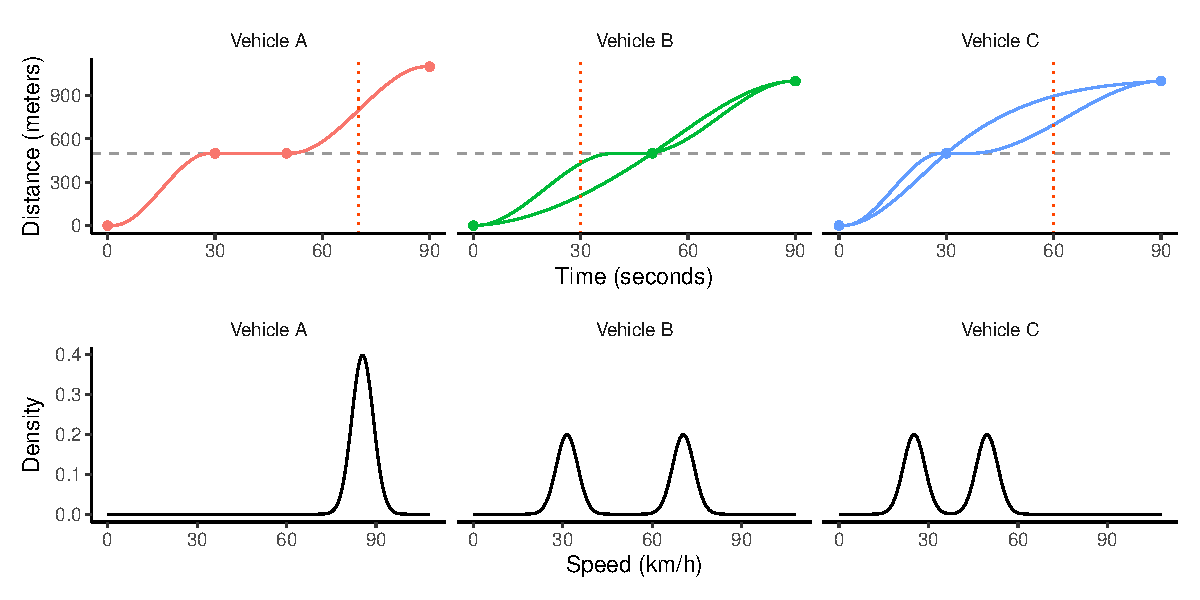
\includegraphics[width=\textwidth]{figure/vobs_multimode-1} 

}

\caption[Demonstration of multimodality in vehicle state]{Uncertainty in whether or not a bus stops can lead to multimodality in its speed dsitribution. Top: observations (points) with possible trajectories which fit the data. The horizontal dashed line represents the location of the stop, and the vertical dotted line indicates the time point at which we wish to estimate vehicle speed. Bottom: estimated speed distribution at the indicated time (dotted vertical line top graph).}\label{fig:vobs_multimode}
\end{figure}


\end{knitrout}


It is evident from the behaviours listed above (described in further detail in section \cref{sec:vehicle_model}) that there are many factors involved in determining a bus' trajectory. Many of these factors, such as speed, are unmeasurable (but can be estimated), while others are often unknowable. An example of the latter is whether or not the bus stopped at a bus stop. \Cref{fig:vobs_multimode} shows a series of \emph{distance} observations\footnote{This is just an example to demonstrate the issue at hand.} for three buses passing a stop:
\begin{itemize}
\item bus A stops and reports both its arrival and departure times;
\item bus B stops, but only reports its departure time;\footnote{This can happen if the arrival bservation is ``lost'' or overwritten by the departure time within the \gls{gtfs} update interval}
\item bus C does not stop and reports a departure time as it passes the stop.
\end{itemize}
Overlaid on the observations are possible trajectory curves for each vehicle: for bus A, there is only one since we observe both the vehicle's arrival and departure. However, B and C each have two potential paths: one in which the vehicle stops, and another in which it does not. The main point is that \emph{we cannot know which is true}. This scenario is an example of \emph{multimodality} in the vehicle's state. In the lower half of \cref{fig:vobs_multimode} are the possible distributions of the vehicles' speeds at the time marked with a dotted vertical line above. For bus A, the distribution is \emph{unimodal}, which satisfies the assumptions of many estimation methods (such as the Kalman filter, \cref{sec:kf}). For buses B and C, however, the speed state is \emph{bimodal}, so the Kalman filter would no longer be an appropriate choice for these data. This multimodality was one of our main reasons for choosing a particle filter to implement our vehicle model.

Once the vehicle's state has been estimated, we can make inferences about the average speed along a given road segment, covered in \cref{sec:vehicle_speeds}. This includes a simulation comparing the variant models introduced in \cref{sec:vehicle_model}, and showing the effectivness of our approach with simulated data. We conclude this chapter with a discussion of the real-time implementation of the model (\cref{sec:particle-filter}), including the process of parameter estimation for the various model parameters, and details of some of the difficulties we experienced modelling these data.



\section{Real-time estimation of vehicle state}
\label{sec:vehicle_model}

Real-time vehicle tracking has been the centre of much research, particularly for robotics applications and self-driving cars \citep{Daum_2005, Gustafsson_2002}. In many of these, data is sampled at a very high frequency, often multiple times per second, leading to high-accuracy estimates of the object's \emph{state}. Alas, with transit data this is seldom the case; instead, it is common for observations to be reported once every 10--30 seconds or, in some cases, even longer.

Low-frequency observations lead to high uncertainties of state parameters and difficulty capturing all possible trajectories, which can lead to degradation of the model and loss of information. In \cref{fig:vobs_multimode}, we show two possible trajectories for buses B and C; there are, in fact, countless possibilities: perhaps the bus waited at the stop a little longer? In this case, there is uncertainty about the bus's dwell time and speed; however, the first step of \agls{rbm} is to \emph{predict} the upcoming state \emph{before observing it} (\cref{sec:recursive-bayes}). If the model does not cover the vehicle's actual trajectory, we effectively ``lose'' the vehicle, and the filter is said to \emph{degenerate} \citep{Chen_2014}. In that case, we typically need to reinitialise the vehicle's state, resulting in a loss of any information we might have gained in the last time step.

When deciding which type of model implementation to use, historically the most common for this type of data is the Kalman filter \citep{Wall_1999, Dailey_2001, Cathey_2003}. However, it assumes a Gaussian state distribution, which I have demonstrated is not the case. Instead, we use a \emph{particle filter} due to its high flexibility and ability to explore a broad set of plausible trajectories \citep{Hans_2015} and excels in situations where there are multiple distinct possiblities, as in \cref{fig:vobs_multimode} \citep{Ulmke_2006}. This makes it well suited for transit modelling, and has been used in many other vehicle tracking applications \citep{Davidson_2011,Gustafsson_2002,Gustafsson_2010,Ulmke_2006}.

\begin{knitrout}\small
\definecolor{shadecolor}{rgb}{0.969, 0.969, 0.969}\color{fgcolor}\begin{figure}

{\centering 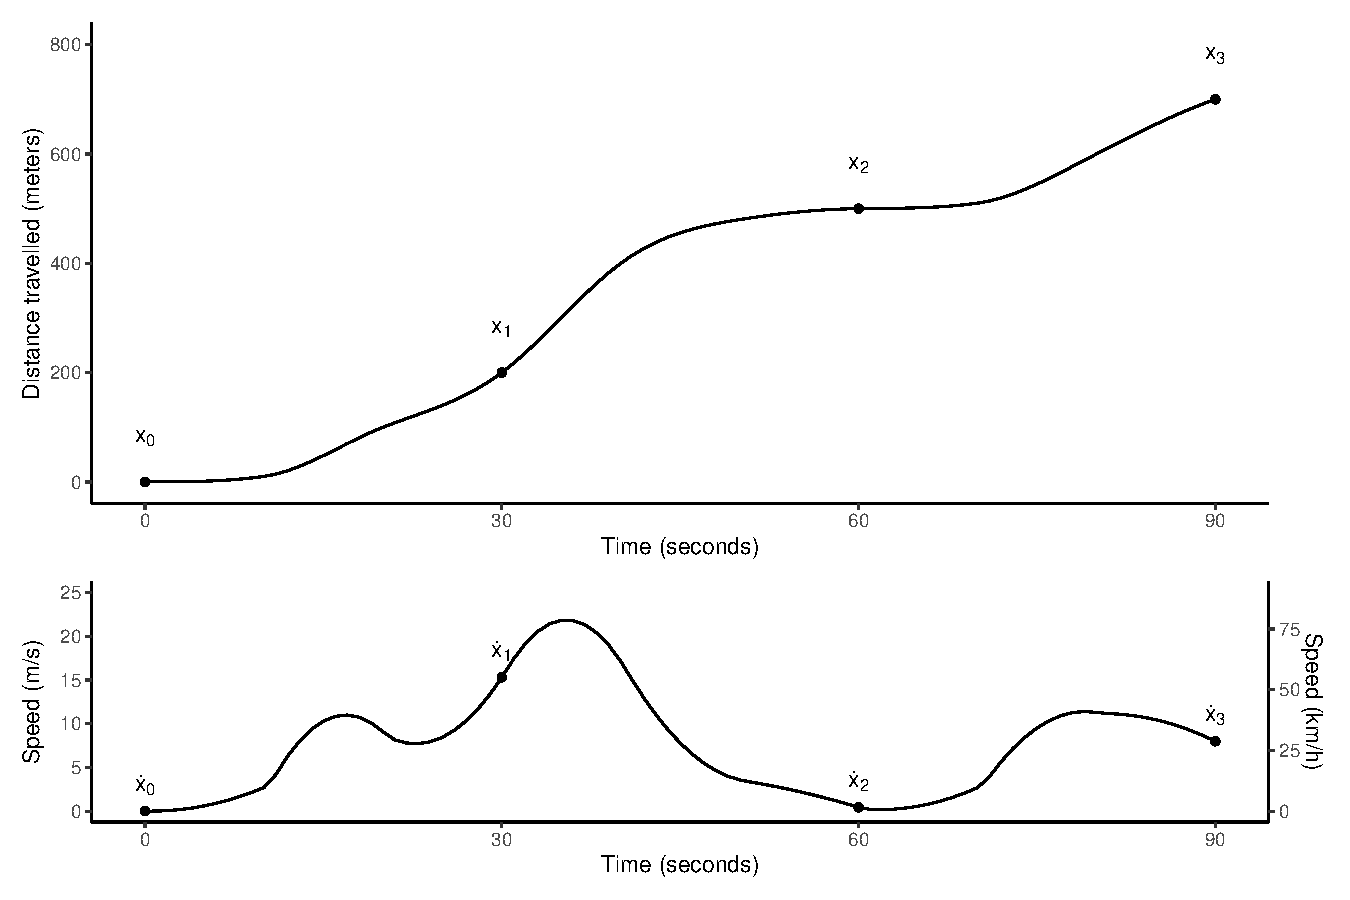
\includegraphics[width=\textwidth]{figure/vehicle_state-1} 

}

\caption[Visualisation of vehicle state showing \emph{distance travelled} and \emph{speed}]{Visualisation of vehicle state showing \emph{distance travelled} and \emph{speed}. The distance travelled, $x$, over time includes points of observed states $\Vstate_k, k=0,\ldots,3$. The gradient of distance over time is speed, $\dot x$: steeper sections of the top graph correspond to higher speeds, and vice verca. The speed graph also includes a second right-hand axis with speed in kilometers per hour (km/h) for reference.}\label{fig:vehicle_state}
\end{figure}


\end{knitrout}

The vehicle model itself involves describing bus behaviour algorithmically to infer the vehicle's \emph{unknown state} $\Vstate_k$ from a sequence of \gls{gps} observations. Since buses service routes with a known path, we represent their position using \emph{distance travelled} along the route's path, which we denote $\Vdist_k$ at time $\Vtime_k$. Additionally, we are interested in the \emph{speed} of the vehicle, $\Vspeed_k$. Therefore, the underlying, unknown, and \emph{unobservable} state of a vehicle at time t is denoted
\begin{equation}
\label{eq:vehicle_state}
\Vstate_k = \tvec{\Vdist_k, \Vspeed_k}.
\end{equation}
\Cref{fig:vehicle_state} graphs a series of vehicle states with time along the x-axis and distance travelled (in meters) along the y-axis. The derivative (gradient) of the curve represents the vehicle's speed. So, for example, the vehicle state at time $t_1 = 30$~seconds is $\Vstate_1 = [\Vdist_1, \Vspeed_1]^\top = [200~\text{m}, 15~\text{m/s}]^\top$. The remainder of this section presents a model, along with a particle filter implementation of it, to estimate vehicle state.

The particle filter represents the vehicle's state using a sample of \emph{particles}, each with an individual state, $\Vstate_k\vi$. We can think of each particle as an ``imaginary bus'' which represents one possible state (and associated trajectory) of the true bus. Together, the particles approximate the posterior distribution of the vehicle's state at time $\Vtime_k$ given all observations up to time $\Vtime_k$, denoted $\Vobs_{1:k}$. The posterior distribution is expressed using the Dirac delta measure, $\dirac$, (\cref{app:dirac-delta-measure}):
\begin{equation}
\label{eq:vehicle_state_dirac}
p(\Vstate_k \cond{} \Vobs_{1:k}) \approx
\sum_{i=1}^\Np \Pwt_{k-1} \dirac_{\Vstate_k\vi}\left(\Vstate_k\right).
\end{equation}

Before implementing \agls{rbm} for these data, we need a \emph{transition function}, a \emph{measurement function}, and a \emph{likelihood}. The transition function, $\Vtrans$, describes how a vehicle behaves between two consecutive observations: that is, the shape of the curves in \cref{fig:vehicle_state}. This allows us to \emph{predict} the future state of the vehicle \emph{given its last known state}. Additionally, we include the \emph{system noise} parameter $\Vnoise$~m/s$^2$, which represents the rate of change of speed. The measurement function, $\Vmeas$, describes the relationship between the vehicle's state, $\Vstate_k$, and the observation of this state, $\Vobs_k$, which is a \gls{gps} location with an associated \emph{measurement error}, $\GPSerr$. We represent this using two simple equations,
\begin{equation}
\label{eq:vehicle_model}
\begin{split}
\Vstate_k &= \Vtrans(\Vstate_{k-1}, \Vnoise), \\
\Vobs_k &= \Vmeas(\Vstate_k) + \GPSerr.
\end{split}
\end{equation}
The \emph{likelihood} function quantifies the plausibility of an observation $\Vobs_k$ given an underlying state $\Vstate_k$.


We now discuss the details of the two components of the model and their implementations. The \emph{prediction step} (\cref{sec:vehicle_model_trans}) supplies an estimate of the bus's state \emph{before observing it} by using a model of bus behaviour. Then the \emph{update state} (\cref{sec:pf-likelihood}) combines the prediction and observation, using the measurement function and likelihood, to obtain a posterior estimate of the vehicle's state.

\subsection{Predicting vehicle state: the transition function}
\label{sec:vehicle_model_trans}

The aim of the prediction step is to obtain a \emph{prior predictive distribution} of the vehicle's state at time $\Vtime_k$ based on its previous state at time $\Vtime_{k-1}$, $p(\Vstate_k \cond{} \Vstate_{k-1})$. Using the model definition in \cref{eq:vehicle_model} along with the particle filter approximation of state in \cref{eq:vehicle_state_dirac}, we can write the prior prediction of the vehicle's state as
\begin{equation}
\label{eq:vehicle_pf_predict}
p(\Vstate_k \cond{} \Vstate_{k-1}) \approx
\sum_{i=1}^\Np
    \Pwt_{k-1}
    \DiracMeasure{\Vstate_k\vi}{\Vstate_k},
\end{equation}
where $\Vstate_k\vi = f(\Vstate\vi_{k-1}, \Vtdiff_k, \Vnoise)$ and $\Vtdiff_k = \Vtime_k - \Vtime_{k-1}$.

The transition function $\Vtrans$ is where we define the vehicle behaviours mentioned earlier. Kalman filter applications are limited to linear transformations of the state which can be expressed in a \emph{transition matrix}. However, \cref{eq:vehicle_pf_predict} shows that, in the case of the particle filter, the transition function is applied to each particle independently, allowing for a lot more flexibility in $\Vtrans$. We now describe the various model components of $\Vtrans$, implemented as an algorithm in the \pkg{transitr} package (see \cref{sec:particle-filter} for details). The core components are vehicle motion (speed and acceleration along a known path), stopping behaviour at known locations (bus stops and intersections), as well as the ability to handle several other scenarios to avoid degeneration.


\subsubsection{Component A: vehicle motion}
\label{sec:vehicle_model_behaviour}

The first behaviour to consider is the vehicle's motion along a known path: the \emph{speed} at which a vehicle is travelling will affect where it ends up. Since speed, $\Vspeed$, is the derivative of distance travelled over time, if $x = d(t)$, then $\Vspeed = d'(t)$, which is shown visually back in \cref{fig:vehicle_state}. It follows that we can predict a vehicle's future state, given its current state (distance travelled and speed) and system noise, $\Vnoise$, which is interpreted as \emph{the average change in speed per second}:
\begin{equation}
\label{eq:vehicle_model_newton}
\Vstate_{k|k-1} = f_{A1}\left(\Vstate_{k-1|k-1}, \Vtdiff_k, \Vnoise\right) =
\begin{bmatrix}
\Vdist_k \\ \Vspeed_k
\end{bmatrix} =
\begin{bmatrix}
\Vdist_{k-1} + \Vtdiff_k\Vspeed_k \\
\Vspeed_{k-1} + v_k
\end{bmatrix}
\end{equation}
where
\begin{equation}\label{eq:vehicle_model_newton_noise}
v_k \sim \TNormal{0}{\Vnoise}{-\Vspeed_{k-1}}{30 - \Vspeed_{k-1}}.
\end{equation}
The noise term is truncated to ensure the new speed is both positive and under 30~m/s, which is 108~km/h (the maximum road speed in Auckland is 100~km/h). The resulting transition function, $\Vtrans_{A1}$, is easily implemented by simulating, for each particle, a new speed before calculating the final state using \cref{eq:vehicle_model_newton}. A similar model was used by \citet{Cathey_2003,Dailey_2001}.


\Cref{fig:transition_demo} demonstrates transition model $\Vtrans_{A1}$ (left) using a sample of $N=10$~particles which, at time $t_{k-1}$, take one of three unique states (due to resampling in the previous iteration, \cref{sec:pf}). The points have been coloured by their initial state to demonstrate the effect of adding system noise \emph{before} transitioning to allow the particles to disperse. Not doing so would, in this instance, yield only three unique states in the final predictive distribution.

\begin{knitrout}\small
\definecolor{shadecolor}{rgb}{0.969, 0.969, 0.969}\color{fgcolor}\begin{figure}

{\centering 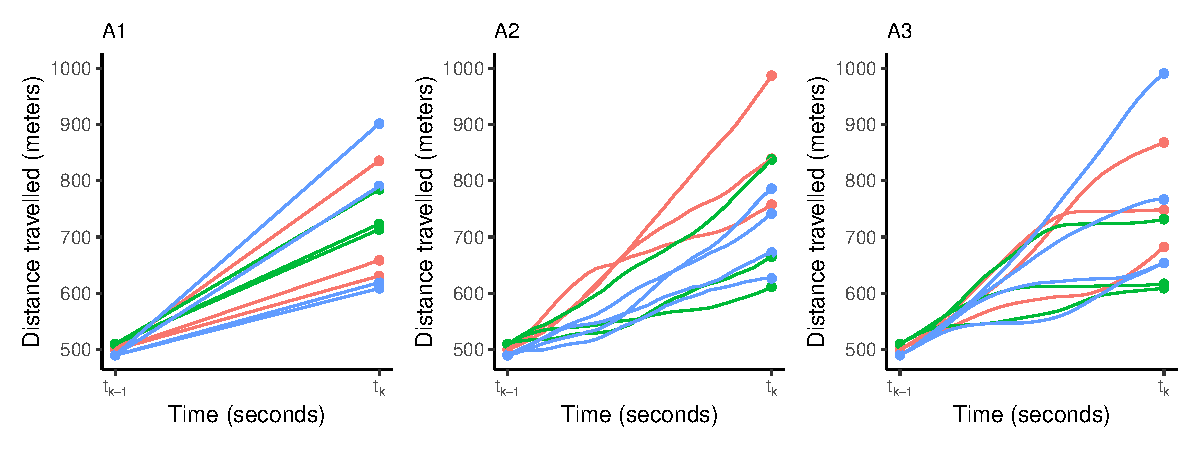
\includegraphics[width=\textwidth]{figure/transition_demo-1} 

}

\caption[Simulated particle trajectories using three transition functions]{Simulated particle trajectories using three transition functions, $f_{A1}$, $f_{A2}$, and $f_{A3}$ from left to right. Points have been coloured by their parent (after resampling) to demonstrate the affect of system noise.}\label{fig:transition_demo}
\end{figure}


\end{knitrout}

The main issue with this model is that it assumes constant speed between observations, which---given Auckland traffic---is unlikely to be the case. In \cref{fig:vehicle_state}, we showed speed varying over time, even between observations. To model this, we \emph{iteratively} update the vehicle's state\footnote{This is one advantage of the particle filter---we can easily perform iterative updates!} by reusing \cref{eq:vehicle_model_newton} $\Vtdiff_k$ times, setting $\Vtdiff_k=1$ in each iteration. The second graph in \cref{fig:transition_demo} shows the effect this has on the particles' trajectories.


Of course, if speed is the first derivative of the vehicle's trajectory function, then \emph{acceleration} is the second, $\Vaccel = d''(t)$. In this case, we add a third component to the vehicle's state and consider speed similarly to distance. The transition function
\begin{equation}
\label{eq:vehicle_model_newton_accel}
\Vstate_{k|k-1} = \Vtrans_{A3}\left(\Vstate_{k-1|k-1},\Vtdiff_k,\Vnoise\right)
\end{equation}
is iterative. It is initialised with $\bz_0 = \Vstate_{k-1|k-1}$ and repeated for $s = 1, \ldots, \Vtdiff_k$ to obtain $\Vstate_{k|k-1} = \bz_{\Vtdiff_k}$:
\begin{equation}
\label{eq:vehicle_model_newton_accel_iter}
\bz_s =
\begin{bmatrix}
z_s \\ z_s \\ z_s
\end{bmatrix} =
\begin{bmatrix}
z_{s-1} + \dot z_s \\
\dot z_{s-1} + \ddot z_s \\
\ddot z_{s-1} + v_s
\end{bmatrix}.
\end{equation}
System noise (interpreted as \emph{the average change in acceleration per second}) is applied to the acceleration term and truncated to ensure the speed remains positive and less than 30~m/s,
\begin{equation}
\label{eq:vehicle_model_accel_dist}
v_s \sim \TNormal{0}{\Vnoise}{-\dot z_{s-1} - \ddot z_{s-1}}{30 - \dot z_{s-1} - \ddot z_{s-1}}.
\end{equation}
These trajectories are shown in the third graph of \cref{fig:transition_demo}. The main issue with $\Vtrans_{A3}$ is that it is difficult to parameterize and constrain the acceleration to ensure speed remains within the interval $(0,30)$ while preserving the function's ability to generate plausible trajectories.



\subsubsection{Component B: stopping at nodes}
\label{sec:vehicle_model_nodes}

In \cref{sec:route-segments}, we discussed using a road network consisting of nodes---either bus stops or intersections---and the roads connecting them. This \emph{segmentisation} allows each route to be expressed as a \emph{sequence of nodes} and connecting \emph{road segments}. Component A of the transition model deals with vehicle behaviour along the road segments; we now examine bus behaviour at nodes.

There are two types of nodes in our framework: \emph{bus stops} where passengers can board and disembark, and \emph{intersections} where buses (and other road users) wait depending on congestion levels and traffic lights. In each case, the bus's behaviour involves:
\begin{enumerate}
\item if the bus stops:
    \begin{enumerate}
    \item deceleration to zero,
    \item wait, and
    \item acceleration to traffic speed;
    \end{enumerate}
\item otherwise, continue as though there is no node.
\end{enumerate}
Only step 1b depends on the type of node.



\paragraph{Bus stops}

A bus's wait time at a bus stop is referred to as \emph{dwell time} and consists of three phases \citep{Hans_2015,Robinson_2013,Meng_2013,Wang_2016}:
\begin{enumerate}[i.]
\item doors open;
\item passengers board and alight; and
\item doors close, and vehicle waits for a gap in the traffic.\footnote{In New Zealand, buses do not get right-of-way, so it is common for them to be stuck for a while in a bus bay.}
\end{enumerate}
Phases i and iii can be combined with 1a and 1c from above (deceleration and acceleration, respectively) into a single parameter, $\mindwell$, which is assumed constant across all buses, stops, and routes.


Phase ii includes the time taken for passengers to get on and off the bus, which varies significantly between stops, routes, and time of day. There are many ways to model service time: an exponential \citep{Hans_2015}, regression models \citep{Shen_2013}, or a real-time Kalman filter \citep{Shalaby_2004}. Here, I present a truncated Normal distribution using the mean and variance of historical dwell times, truncated at zero. The service time at stop $m$ along a route ($m=1,...,M-1$; dwell time does not apply to the last stop) is denoted $\pserve_m$, modelled by its mean and variance, $\dwell_m$ and $\dwellvar_m$, respectively, as estimated from historical data:
\begin{equation}
\label{eq:stop_dwell_time}
\pserve_m \sim \TNormal{\dwell_m}{\dwellvar_m}{0}{\infty}.
\end{equation}

For each bus stop, we also have a \emph{stopping probability} $\Prstop_m\in(0,1)$. For the first and last stops, $m\in\{1,M\}$, this is unity; for the remainder, we have no data with which we can reliably estimate $\Prstop_m$, so, for now, we assume all stops have the same values specified by a global $\Prstop$ parameter (see \cref{sec:pf_params} for details on this). The outcome of whether a bus stops at a bus stop, $p_m$, is a Bernoulli trial,
\begin{equation}
\label{eq:stop_pstop}
\Istop_m \sim \Bern{\Prstop_m}.
\end{equation}
The total dwell time of a bus at stop $m$ can be expressed as
\begin{equation}
\label{eq:stop_total_dwell_time}
\pdwell_m = \Istop_m (\mindwell + \pserve_m),
\end{equation}
which, under the particle filtering framework, is straightforward to implement. \Cref{fig:eta_dwell_times} displays the dwell time distribution at a stop.


\begin{knitrout}\small
\definecolor{shadecolor}{rgb}{0.969, 0.969, 0.969}\color{fgcolor}\begin{figure}

{\centering 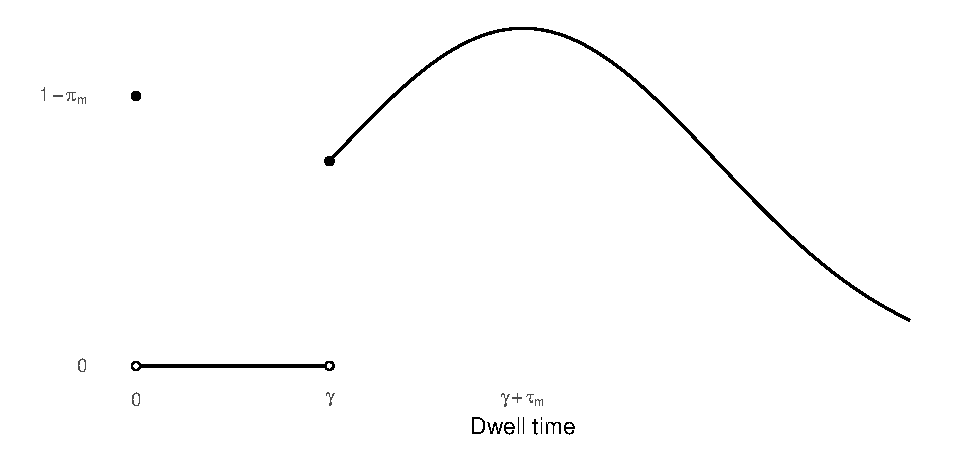
\includegraphics[width=.8\textwidth]{figure/eta_dwell_times-1} 

}

\caption[The \gls{pdf} of dwell time at a stop]{The \gls{pdf} of dwell time at bus stop $m$.}\label{fig:eta_dwell_times}
\end{figure}


\end{knitrout}


One other scenario for bus stops is a \emph{layover}, which is when a bus arrives early at a major stop\footnote{This is more common on longer routes in an attempt to keep them to schedule.} and waits until the scheduled departure time. In the \gls{gtfs} stop times table, layovers are denoted by an arrival time earlier than the corresponding departure time, as shown in \cref{tab:layover_times}. Again, under the particle filtering framework, this is simple enough to implement: if the particle arrives early, it waits until the scheduled departure time before leaving. However, it is not always the case that buses will wait for the layover, so we add a probability of adherence, similar to the stopping probability in \cref{eq:stop_pstop}. However, since this has greater implication for arrival time prediction, we defer the details for \cref{cha:prediction}.

\begin{knitrout}\small
\definecolor{shadecolor}{rgb}{0.969, 0.969, 0.969}\color{fgcolor}\begin{table}

\caption[Arrival times for a trip with a layover]{\label{tab:layover_times}Arrival times for a trip with a layover stop (marked with an asterix, $\star$). This is indicated in the \gls{gtfs} data by a departure time later than the arrival (in this case the difference is one second).}
\centering
\fontsize{8}{10}\selectfont
\begin{tabular}[t]{rll}
\toprule
Stop & Arrives & Departs\\
\midrule
1 & 19:30:00 & 19:30:00\\
2 & 19:30:36 & 19:30:36\\
3 & 19:31:33 & 19:31:33\\
4 & 19:32:04 & 19:32:04\\
5 & 19:32:59 & 19:33:00 *\\
6 & 19:33:42 & 19:33:42\\
7 & 19:34:14 & 19:34:14\\
\bottomrule
\end{tabular}
\end{table}


\end{knitrout}




\paragraph{Intersections}

Modelling intersections is much the same as bus stops, with a few differences:
\begin{enumerate}[i.]
\item the bus doors do not open, passengers do not get on or off, so there is no longer a $\gamma$ parameter;
\item the bus does not necessarily stop at the node location, since there may be a queue;
\item depending on the length of the queue and the type of intersection, the bus may require more than one ``light phase'' to pass through the intersection (for traffic lights), OR the bus may creep forward slowly (at uncontrolled (give-way) intersections and roundabouts).
\end{enumerate}
However, we had no reliable intersection location information available, so were unable to explore this component of the model thoroughly. Instead, I describe here a single behaviour but note that it could easily be modified in the future.

We model the wait time $w$ at intersection $\ell$ with an exponential distribution with rate $\intwait_\ell^{-1}$:
\begin{equation}
\label{eq:int_wait}
\pcwait_\ell \sim \Exp{\intwait_\ell^{-1}}.
\end{equation}
As at bus stops, the stopping outcome $\Iint_\ell$ is a Bernoulli trial with probability $\rho_\ell$,
\begin{equation}
\label{eq:int_stop_bern}
\Iint_\ell \sim \Bern{\rho_\ell},
\end{equation}
leading to an overall wait time of
\begin{equation}
\label{eq:int_total_wait}
\pwait_\ell = \Iint_\ell \pcwait_\ell.
\end{equation}
However, from point iii above, once the wait time is over, we conditionally allow the bus to move forward with the possibility of stopping again. In practice, this would be proportional to the distance of the vehicle from the intersection and other factors. As mentioned in \cref{sec:vp_data}, this is not as easy as it seems since observations may be linked to a waypoint at the intersection\footnote{Actually, in the middle of it.} instead of where the bus is, so we cannot determine the bus's distance from the intersection reliably.

\subsection{Likelihood}
\label{sec:pf-likelihood}

The second component of \gls{rbe} is the update step, which involves accounting for the likelihood of the data given the predicted state, $p(\Vobs_k | \Vstate_k)$. In the \pf{}, as discussed in \cref{sec:pf}, updating is performed by reweighting each of the particles based on their likelihoods, $p(\Vobs_k | \Vstate\vi_k)$, and then, if necessary, performing weighted resampling with replacement (importance resampling). That is,
\begin{equation}
\label{eq:vehicle_pf_update}
p(\Vstate_k | \Vobs_{1:k}) \approx
\sum_{i=1}^\Np
    \Pwt_{k}
    \DiracMeasure{\Vstate\vi_k}{\Vstate_k}
\end{equation}
where
\begin{equation}
\label{eq:vehicle_pf_reweight}
\Pwt_k = \frac{
    \Pwt_{k-1} p(\Vobs_k | \Vstate\vi_k)
}{
    \sum_{j=1}^\Np \Pwt[j]_{k-1} p(\Vobs_k | \Vstate\vi[j]_k)
}
\end{equation}


The likelihood function is where the \pf{} is superior in this application. Were we to model the vehicle's state with a \kf{}, we would need to somehow compare a distribution in one dimension (distance travelled) with an observation in two dimensions (\gls{gps} coordinate). \cite{Cathey_2003} used an optimisation technique to obtain an estimated observation of distance travelled based on the observation location, which they then used as data for their \kf{} implementation. However, as demonstrated in \cref{fig:lhood_obs}, there are situations where the ``maximised'' location may be wrong, in which case the resulting state will be eroneous.


The \pf{} effectively checks to see how plausible the observation is assuming each particle is the truth, allowing us to weight each particle by its plausibility. Since there are two types of data, two likelihood functions are required: one for \GPS{} observations, and a second for trip updates. There is no need to match the observations to distance: instead, each particle's state can be transformed into a \gls{gps} coordinate, making it directly compariable to the vehicle's reported location.


\subsubsection{GPS vehicle locations}
\label{sec:lhood_gps}

\begin{knitrout}\small
\definecolor{shadecolor}{rgb}{0.969, 0.969, 0.969}\color{fgcolor}\begin{figure}
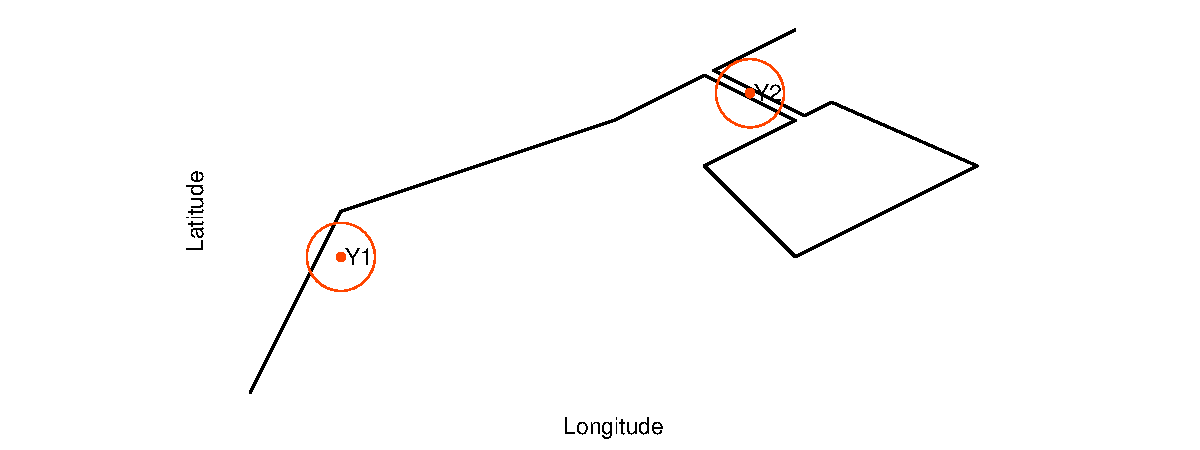
\includegraphics[width=\maxwidth]{figure/lhood_obs-1} \caption[Observations of vehicle on a simple path]{Observations of vehicle on a simple path. The red points indicate the reported GPS positions, with circles indicating the GPS error associated with each observation. Observation Y1 is easy to map to the route, while Y2 is more complicated and has two plausible, distinct locations.}\label{fig:lhood_obs}
\end{figure}


\end{knitrout}





For the \gls{gps} location update, the inherent \gls{gps} error, $\GPSerr$, needs to be filtered out to get better estimates of vehicle state. Examples of positions are shown in \cref{fig:lhood_obs}. A particle's likelihood should represent the geographical \emph{closeness} of the estimated position to the vehicle's reported position. We therefore want the likelihood to depend on the \emph{distance between the observed and predicted} vehicle locations. The first step to computing the likelihood is therefore
to calculate the GPS position of the \emph{particle}, $\Ppos\vi_k$, by using the \emph{measurement function},
\begin{equation}
\label{eq:pf_measurement_fun}
\Ppos\vi_k = \Vmeas(\Vstate\vi_k, \ShapePath)
\end{equation}
which is simply a deterministic function given the route's path, $\ShapePath$, which is a sequence of latitude-longitude pairs and the cumulative distance along the line. Once the geographical position of the particle is obtained, it is compared to the observed vehicle location, as shown in \cref{fig:gps_dist}.

\begin{knitrout}\small
\definecolor{shadecolor}{rgb}{0.969, 0.969, 0.969}\color{fgcolor}\begin{figure}

{\centering 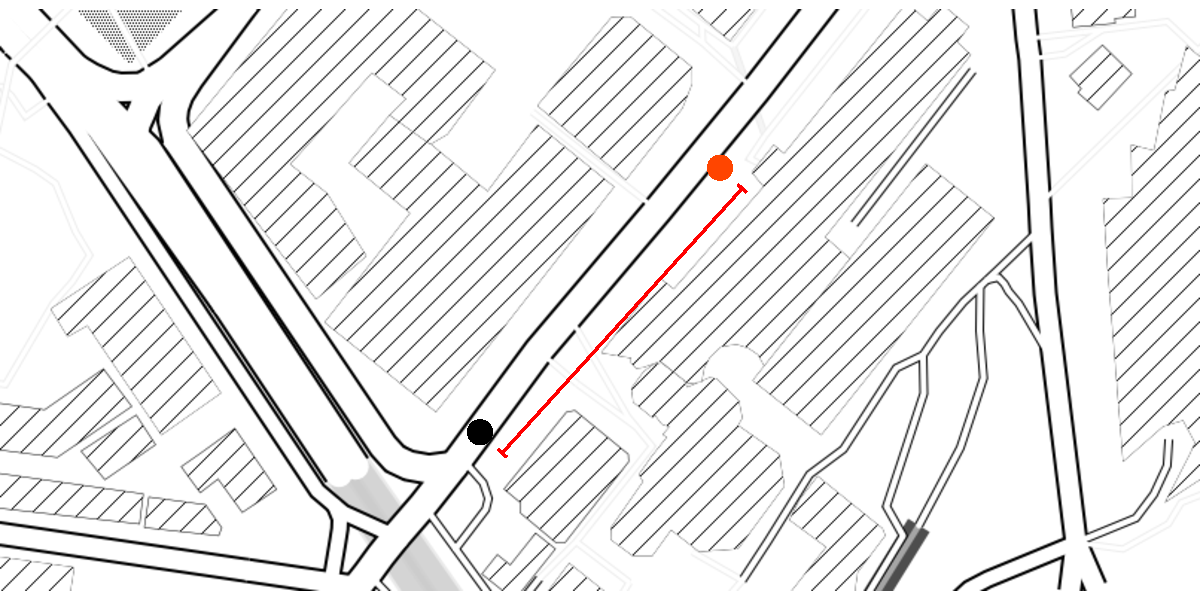
\includegraphics[width=0.8\textwidth]{figure/gps_dist-1} 

}

\caption[GPS distance between two points]{GPS distance between two points. The vehicle's reported location is shown in orange; one particle estimate of it's location is in black. The desired distance is denoted by the red line.}\label{fig:gps_dist}
\end{figure}


\end{knitrout}

Computing the distance between two GPS coordinates can achieved using several formulae, each with varying levels of accuracy. Since all of the distances are going to be (very) small, the \emph{Equirectangular projection} is sufficiently accurate for computing geographical distances \citep{cn}. This projection transforms the point $\Vobs_1 = \tvec{\Vlon_1, \Vlat_1}$, where latitude $\Vlat$ and longitude $\Vlon$ are in radians (the width of one longitudinal radian depends on latitude) onto a surface with meters on both axes, centered on the point $\Vobs_0 = \tvec{\Vlon_0, \Vlat_0}$ and using the Earth's radius $R = 6.371 \times 10^6$m,
\begin{equation}
\label{eq:equirectangular_projection}
\Vproj{\Vobs_1}{\Vobs_0} =
\begin{bmatrix} x \\ y \end{bmatrix} =
R \begin{bmatrix}
(\Vlon_1 - \Vlon_0) \cos \Vlat_0 \\
(\Vlat_1 - \Vlat_0)
\end{bmatrix}
\end{equation}
so that the distance between the points can easily be computed
using their \emph{euclidean distance}
\begin{equation}
\label{eq:obs_dist}
\dist{\Vobs_0, \Vobs_1} = \sqrt{x^2 + y^2}.
\end{equation}
This is shown visually in \cref{fig:gps_projection}.
Note that conversion from degrees to radians is achieved by
multiplying degrees by $\frac{\pi}{180}$.

\begin{knitrout}\small
\definecolor{shadecolor}{rgb}{0.969, 0.969, 0.969}\color{fgcolor}\begin{figure}

{\centering \subfloat[GPS coordinates\label{fig:gps_projection1}]{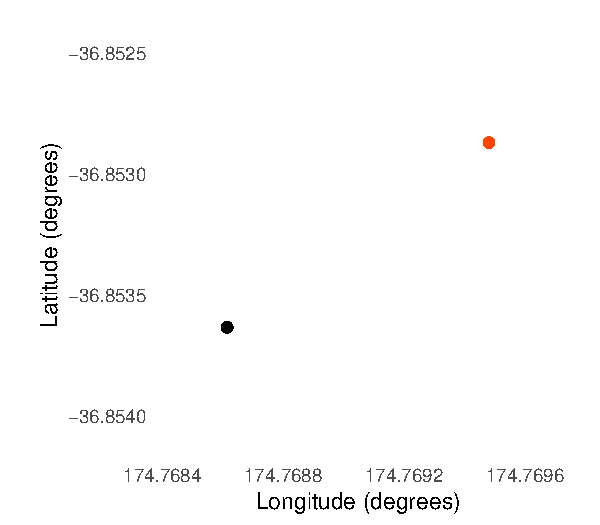
\includegraphics[width=0.49\textwidth]{figure/gps_projection-1} }
\subfloat[Projected points\label{fig:gps_projection2}]{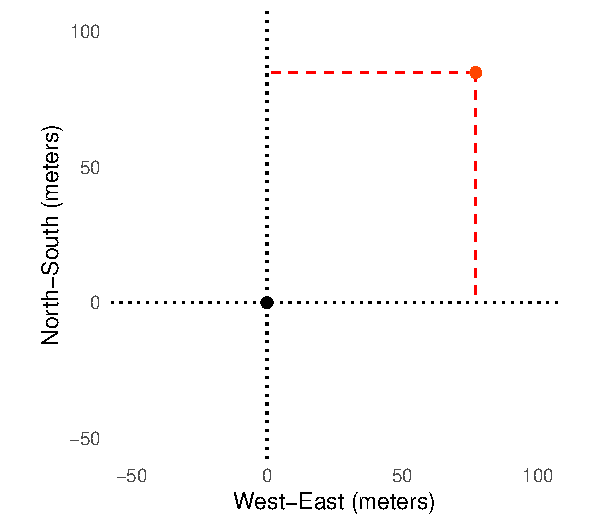
\includegraphics[width=0.49\textwidth]{figure/gps_projection-2} }

}

\caption[Equirectangular projection of GPS coordinates onto flat surface, allowing the distance from each particle to the observed location to easily be calculated]{Equirectangular projection of GPS coordinates onto flat surface, allowing the distance from each particle to the observed location to easily be calculated.}\label{fig:gps_projection}
\end{figure}


\end{knitrout}


Now that spherical observations can be compared on a flat surface,
it is necessary to assume that \GPS{} observations are distributed
as a multivariate random variable around the true position of the vehicle
on the ground,
with a \GPS{} error of $\GPSerr$,
and that the variation does not depend on direction.
That is, if the observation $\Vobs_k$ is projected using
\cref{eq:equirectangular_projection} conditional on the true position
$\Vmeas(\Vstate_k)$,
then the projected point will be a multivariate random variable
$\vec{r}_k \sim \Normal{\vec{0}}{\GPSerr \mat{I}}$.
The above, shown in \cref{fig:gps_error2},
can more simply be expressed by
\begin{equation}
% \label{eq:obs_projection}
\label{eq:gps_error_model}
\Vproj{\Vobs_k}{\Vmeas(\Vstate_k)} =
    \Vproj{\Vmeas(\Vstate_k)}{\Vmeas(\Vstate_k)} + \vec{r}_k
    = \vec{r}_k
\end{equation}

% \begin{equation}
% \Vobs_k = \Viproj{\vec{r}\vi_k}{\Vmeas(\Vstate\vi_k)}.
% \end{equation}

\begin{knitrout}\small
\definecolor{shadecolor}{rgb}{0.969, 0.969, 0.969}\color{fgcolor}\begin{figure}

{\centering \subfloat[GPS map error\label{fig:gps_error1}]{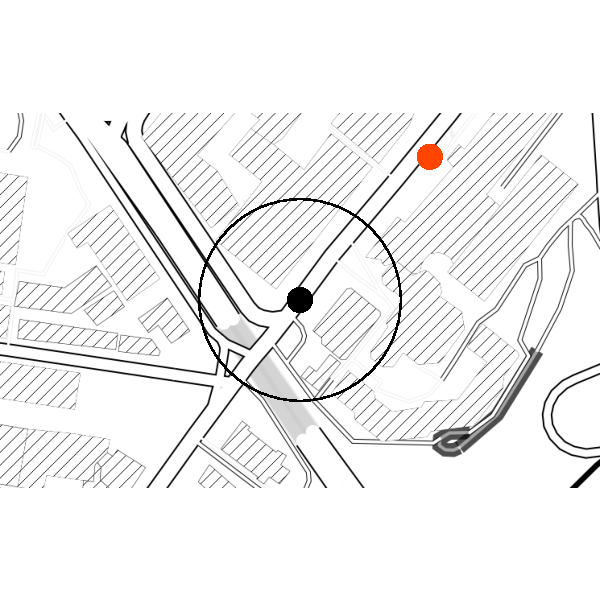
\includegraphics[width=0.49\textwidth]{figure/gps_error-1} }
\subfloat[Projected error\label{fig:gps_error2}]{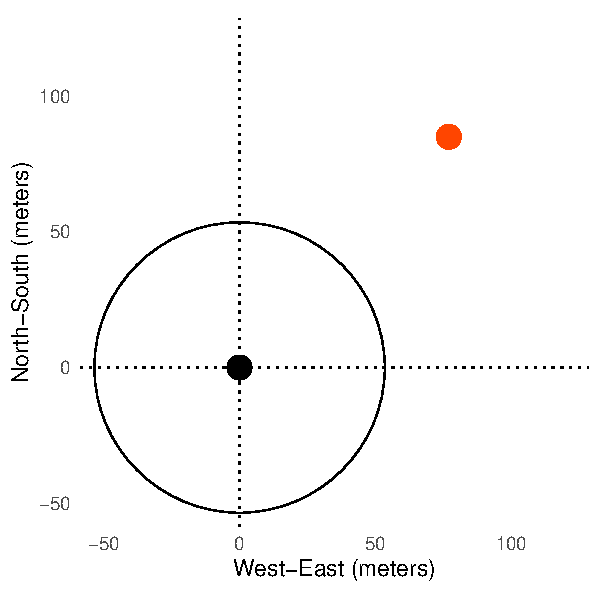
\includegraphics[width=0.49\textwidth]{figure/gps_error-2} }

}

\caption[GPS error is assumed to be circular on a map]{GPS error is assumed to be circular on a map.}\label{fig:gps_error}
\end{figure}


\end{knitrout}


From \cref{eq:equirectangular_projection,eq:obs_dist,eq:gps_error_model}
the distance between the true and observed locations
is the magnitude of the error $\vec{r}_k$,
\begin{equation}
\dist{\Vobs_k, \Vmeas(\Vstate_k)} = ||\vec{r}_k|| =
    \sqrt{r_{k1}^2 + r_{k2}^2}
\end{equation}
However, this error can also be expressed in terms of two independent,
standard normal random variables $z_1, z_2 \sim \Normal{0}{1}$,
such that $r_{jk} = \GPSerrSD z_j$ for $j = 1, 2$,
resulting in
\begin{equation}
\dist{\Vobs_k, \Vmeas(\Vstate\vi_k)} =
    \sqrt{(\GPSerrSD z_1)^2 + (\GPSerrSD z_2)^2} =
    \GPSerrSD \sqrt{z_1^2 + z_2^2}
\end{equation}
Since the distribution of two squared standard normal random variables is known
to be $\chi^2$ distributed with 2~degrees of freedom,
which is itself exponential with rate 0.5
\citep{cn},
then
\begin{equation}
\label{eq:sum_sq_dist}
z_1^2 + z_2^2 \sim \Exp{\frac{1}{2}}
\end{equation}
which, following the [fact] that if $X \sim \Exp{\theta}$,
then $cX \sim \Exp{\frac{\theta}{c}}$,
the squared distance between points is simply represented as
\begin{equation}
\label{eq:distance_distrib}
\dist{\Vobs_k, \Vmeas(\Vstate_k)}^2 \sim \Exp{\frac{1}{2\GPSerr}}
\end{equation}

So now, given a particle state estimate of $\Vstate\vi_k$,
the likelihood of a \GPS{} observation using only
the distance between two coordinates is given by
\begin{equation}
\label{eq:particle_lh_fun}
p(\Vobs_k | \Vstate\vi_k) =
    \frac{1}{2\GPSerr} \exp\left\{
        - \frac{\dist{\Vobs_k, \Vmeas(\Vstate\vi_k)}^2}{2\GPSerr}
    \right\}
\end{equation}
allowing the particles to be reweighted using \cref{eq:vehicle_pf_reweight}.
This is shown visually in \cref{fig:pf_wts}.


\begin{knitrout}\small
\definecolor{shadecolor}{rgb}{0.969, 0.969, 0.969}\color{fgcolor}\begin{figure}

{\centering 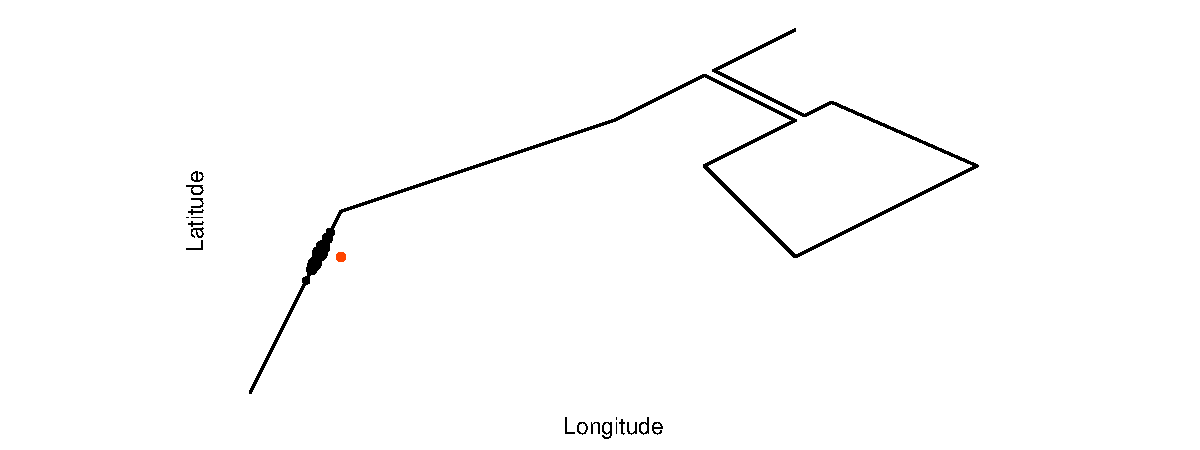
\includegraphics[width=\maxwidth]{figure/pf_wts-1} 

}

\caption[The \pf{} estimate of vehicle state after reweighting particles based on the likelihood, or distance from the observed location]{The \pf{} estimate of vehicle state after reweighting particles based on the likelihood, or distance from the observed location.}\label{fig:pf_wts}
\end{figure}


\end{knitrout}


\subsubsection{Trip updates}
\label{sec:lhood_trip}

As well as vehicle position updates from \GPS{} data, \GTFS{} provides trip updates from arrival and departure information. In many situations, it is difficult to infer a vehicle's trajectory based solely on \GPS{} data, and so trip updates are therefore an invaluable part of the update step. In this case, the \pf{} prediction step goes ahead as presented in \cref{sec:vehicle_model_trans}, but instead of then comparing the coordinates, the arrival or departure times are used to compute the liklelihood of the particles.


The trip update observations differ from the \GPS{} observations in that there are now three situations which can occur. The observation can be of an arrival time at stop $m$, $\Varr_m$, or it can be of a departure time, $\Vdep_m$. In the latter case, treatment of the observations depends on whether or not $\Varr_m$ was observed. This gives us three likelihood functions to derive,
\begin{itemize}
\item $p(\Varr_m | \Vstate_k)$, the arrival time likelihood function,
\item $p(\Vdep_m | \Vstate_k, \text{arrival missing})$, the departure time likelihood conditional
    on not having observed arrival time, and
\item $p(\Vdep_m | \Vstate_k, \text{arrival observed})$, the departure time likleihood conditional
    on having observed arrival time.
\end{itemize}


To compute the likelihood for these, we refer back to the dwell time model described in \cref{eq:stop_dwell_model,eq:stop_dwell_time}. Two additional parameters are also needed: the actual arrival time of the bus at stop $m$, $\Tarr_{m}$, and the measurement error of arrival time in seconds, $\TUerr$. The arrival time can be computed for each stop $m$ directly from the model (i.e., via interpolation). The departure time is then computed by summing the arrival and dwell times.


The observed arrival and departured times, denoted $\Varr_m$ and $\Vdep_m$, respectively, are assumed to each be normally distributed, with mean and variance determined by the described model. For arrival time, this is simply
\begin{equation}
\label{eq:tu_arr_lhood}
\Varr_m \sim \Normal{\Tarr_{mr}}{\TUerr}.
\end{equation}
and for departure time,
\begin{equation}
\label{eq:tu_dep_lhood}
\Vdep_m \sim \Normal{\Tarr_m + \pdwell_m}{\TUerr}
\end{equation}


In our \pf{} implementation, each observation will be processed individually; in situations where more than one type of observation is recieved, they are processed in chronological order and the particles reweighted between each. The necessary likelihood component for \cref{eq:vehicle_pf_reweight} is therefore
\begin{equation}
\label{eq:tu_obs_lhood}
p(\Vobs_k | \Vstate\vi_k) =
\begin{cases}
\frac{1}{\sqrt{2\pi\TUerr}}
    \exp\left\{
        -\frac{(\Varr_m - \Tarr_m)^2}{2\TUerr}
    \right\} & \text{for arrival times} \\
\frac{1}{\sqrt{2\pi\TUerr}}
    \exp\left\{
        -\frac{(\Vdep_m - \Tarr\vi_m - \pdwell\vi_m)^2}{2\TUerr}
    \right\} & \text{for departure times}
\end{cases}
\end{equation}
which allows the particle sample to be reweighted according to the temporal difference in arrival and departure times. This is demonstrated in \cref{fig:tu_update}.

\begin{knitrout}\small
\definecolor{shadecolor}{rgb}{0.969, 0.969, 0.969}\color{fgcolor}\begin{figure}

{\centering 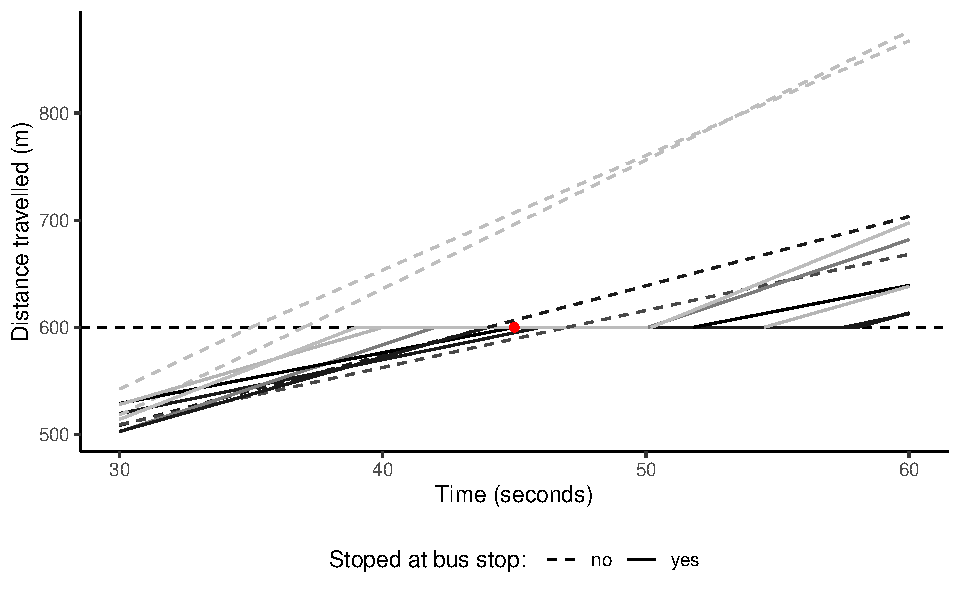
\includegraphics[width=0.8\textwidth]{figure/tu_update-1} 

}

\caption[Particle's travelling past an intermediate stop with an arrival time observation (red point)]{Particle's travelling past an intermediate stop with an arrival time observation (red point). Solid lines represent particles that stopped, while dashed lines indicate the particle drove straight past the stop. The lines are coloured by their resepective weights according to the likelihood based on the observed arrival time (red dot), where greyer lines have less weight.}\label{fig:tu_update}
\end{figure}


\end{knitrout}


\section{Estimating road speeds}
\label{sec:vehicle_speeds}

Now that we have estimated the necessary vehicle states and their respective trajectories, we can infer each vehicle's \emph{average speed} along road segment $\ell$ of its current route, $\Vtt_{\ell}$. These estimates are later used to update the \emph{road network state} (\cref{cha:network_model}) and ultimately estimate arrival times (\cref{cha:prediction}).


Estimation of average road speed is performed by first computing the \emph{travel time} along each road segment as the bus traverses the network. To do so, we record the time when the vehicle starts and ends each segment, $\Vsegstart_\ell$ and $\Vsegend_\ell$, respectively, and take the difference to obtain the travel time in seconds. By using a particle filter, we record these values for each particle as it is transitioned to each new state. Finally, transforming to average speed uses the length of the segment, $\Tseglen_\ell$, in meters, and the standard speed formula ($\text{speed} = \frac{\text{distance}}{\text{time}}$):
\begin{equation}
\label{eq:vehicle_avg_speed}
\Vtt\vi_\ell = \frac{\Tseglen_\ell}{{\Vsegend}\vi_\ell - {\Vsegstart}\vi_\ell}.
\end{equation}


Since estimating \cref{eq:vehicle_avg_speed} is straightforward for each particle, the posterior distribution of the vehicle's average travel time along segment $\ell$, given all observations up to and including time $\Vtime_k$, is approximated using the Dirac delta measure,
\begin{equation}
\label{eq:pf_speed_dist}
p(\Vtt_\ell \cond{} \Vobs_{1:k}) \approx
\sum_{i=1}^\Np \Pwt_k \DiracMeasure{\Vtt\vi_\ell}{\Vtt_\ell}.
\end{equation}
In situations where only some particles have completed travel along a segment, the application waits until the next iteration to re-check that all particles have completed it and, if so, the average speed is calculated.


\subsection{Simulation study}
\label{eq:pf_simulation_study}

To assess the accuracy of the models presented in \cref{sec:vehicle_model}, vehicle simulations were performed with known road speeds while tracking the vehicle along the route. Three different sampling methods were used to obtain observations:
\begin{itemize}
\item uniform sampling with 10~second intervals;
\item uniform sampling with 30~second intervals; and
\item non-uniform sampling at nodes.
\end{itemize}
As mentioned in \cref{sec:vp_data}, the last of these is, in fact, a common feature of the Auckland Transport data; we discuss the complications further in \cref{sec:pf_implementation}. In each simulation, we implemented the three variations of the transition function: $\Vtrans_{A1}$, $\Vtrans_{A2}$, and $\Vtrans_{A3}$.


The posterior mean travel time was used to examine and compare the estimation accuracy of the models, which is simple to calculate from the particle filter estimates of travel time using the weighted mean of the sample (\cref{app:particle-summaries}):
\begin{equation}
\label{eq:pf_travel_time_mean}
\bar\Vtt_\ell =
\E{\Vtt_\ell | \Vobs_{1:k}} =
\sum_{i=1}^\Np \Pwt_k \Vtt\vi_\ell.
\end{equation}


To evaluate and compare the estimation performance of the models, we use \gls{rmse} and \gls{mae} (defined in \cref{app:error-functions}).


\subsubsection{Simulation A: general vehicle model}
\label{sec:vehicle_sim_A}





The simulated data, shown in \cref{fig:sim1_graph}, uses the transition model described by $\Vtrans_{A3}$ to simulate a vehicle trajectory ignoring bus stops. Observations are obtained using three sampling methods: uniform sampling with high and low frequency, and non-uniform sampling, which is more in line with how the Auckland Transport data is collected.


The goal of the simulation is to estimate the vehicle's average speed along several road segments, as well as the associated uncertainty. The simulation was performed in \Rstats{} \citep{rcore} using $\Np = 2000$ particles per vehicle, and so the implementation is slightly different from the \Cpp{} one defined in \cref{sec:pf_implementation}.

\begin{knitrout}\small
\definecolor{shadecolor}{rgb}{0.969, 0.969, 0.969}\color{fgcolor}\begin{figure}
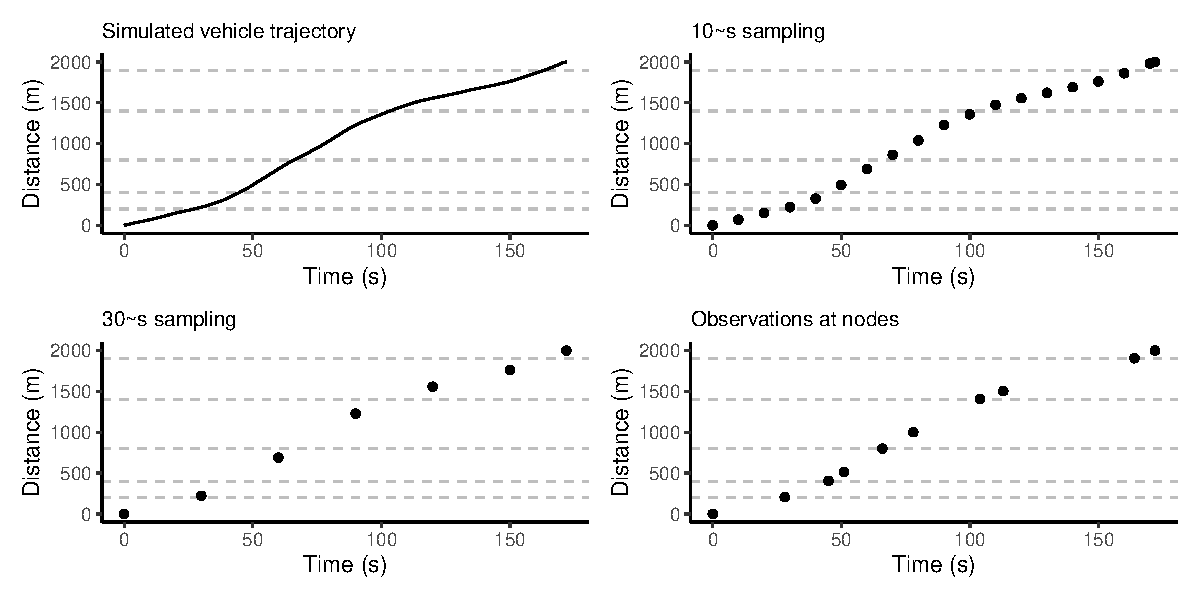
\includegraphics[width=\linewidth]{figure/sim1_graph-1} \caption[Vehicle trajectory with sampled observations for simulation A]{A simulated vehicle trajectory (top left) for simulation A along five road segments (dashed grey lines). Observations are sampled using three techniques (see text).}\label{fig:sim1_graph}
\end{figure}


\end{knitrout}

\begin{knitrout}\small
\definecolor{shadecolor}{rgb}{0.969, 0.969, 0.969}\color{fgcolor}\begin{figure}
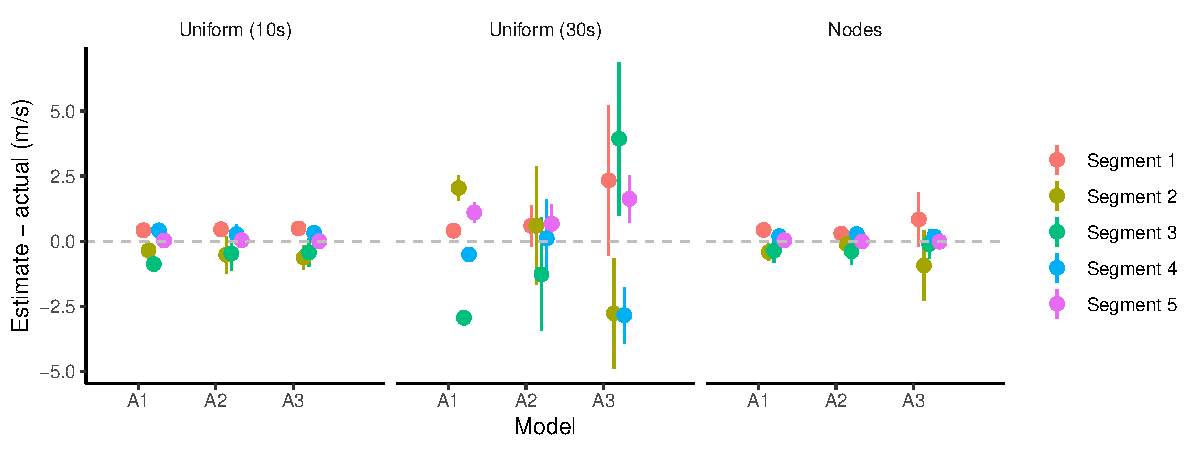
\includegraphics[width=\linewidth]{figure/sim1_pf-1} \caption[Results for simulation A]{Simulation A results for the three models (A1, A2, A3) applied to the data from three sampling methods using $\Np=2000$ particles. Shown is the travel time prediction error along with its standard deviation.}\label{fig:sim1_pf}
\end{figure}


\end{knitrout}


The results of the simulation applied to the data displayed in \cref{fig:sim1_graph} is shown in \cref{fig:sim1_pf}. Under the high-frequency uniform sampling method, all models perform similarly with high precision (the errors are all close to zero) and accuracy (the uncertainty is small enough that the error bars are barely visible). For the low-frequency sampling, however, model A2 shows slightly better precision than A1 and A3. Finally, for sampling at nodes, the models all perform similarly.



To further examine the comparative performance of the models, we repeated the simulation 100~times using the same segments and sampling points, but varying the underlying trajectory of the vehicle, with the results displayed in \cref{fig:sim1_pf_full}. Models A1 and A2 have better accuracy than A3. Most obviously, however, is that the sampling rate significantly affects accuracy. An overall comparison of \gls{rmse} and \gls{mae} are displayed in \cref{tab:sim1_pf_full}, which affirms the findings that A3 is less accurate than the other methods  (except under high-frequency sampling where they all perform similarly).


\begin{knitrout}\small
\definecolor{shadecolor}{rgb}{0.969, 0.969, 0.969}\color{fgcolor}\begin{figure}
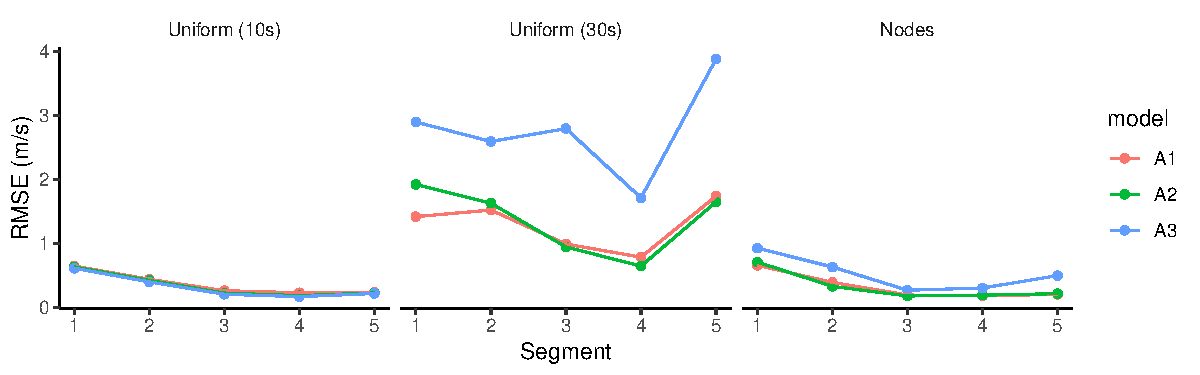
\includegraphics[width=\linewidth]{figure/sim1_pf_full-1} \caption[Results for simulation A replicated 100~times]{Speed estimation results for 100 simulations. In each the vehicle trajectory was simulated using a different seed and speed estimated by the mean of the particles, which is compared to the true speed using \gls{rmse}.}\label{fig:sim1_pf_full}
\end{figure}

\begin{table}

\caption{\label{tab:sim1_pf_full}RMSE and MAE of average speed estimation for simulation A for three models and three sampling techniques.}
\centering
\fontsize{8}{10}\selectfont
\begin{tabular}[t]{llrr}
\toprule
Sampling method & Model & RMSE (m/s) & MAE (m/s)\\
\midrule
Uniform (10s) & A1 & 0.40 & 0.27\\
 & A2 & 0.38 & 0.26\\
 & A3 & 0.36 & 0.24\\
\midrule
Uniform (30s) & A1 & 1.34 & 0.95\\
 & A2 & 1.44 & 1.01\\
 & A3 & 2.87 & 2.07\\
\midrule
Nodes & A1 & 0.38 & 0.25\\
 & A2 & 0.38 & 0.25\\
 & A3 & 0.58 & 0.36\\
\bottomrule
\end{tabular}
\end{table}


\end{knitrout}



\subsubsection{Simulation B: bus stop model}
\label{sec:vehicle_sim_B}

In the previous simulation, we assumed the vehicle travelled along the route without stopping. Now, we add bus stop behaviour to the model, as shown in \cref{fig:sim2_graph}. In the simulated data, the bus stops at all stops with unknown dwell time, and we use $\pi=0.5$ for the stopping probability in the particle filter when estimating vehicle state. The sampling is the same as before: 10~second and 30~second rates, as well as observations at nodes (intersections and bus stops). In this simulation, models B1, B2, and B3 are modified versions of A1, A2, and A3, respectively, but include bus stopping behaviour from \cref{sec:vehicle_model_nodes}.




\afterpage{\clearpage}

The results of the second simulation are shown in \cref{fig:sim2_pf}, where we see somewhat similar results as before: the models perform equally well under high-frequency uniform sampling, with lower precision and accuracy under low-frequency sampling. For sampling at nodes, the models perform similarly.

\begin{knitrout}\small
\definecolor{shadecolor}{rgb}{0.969, 0.969, 0.969}\color{fgcolor}\begin{figure}
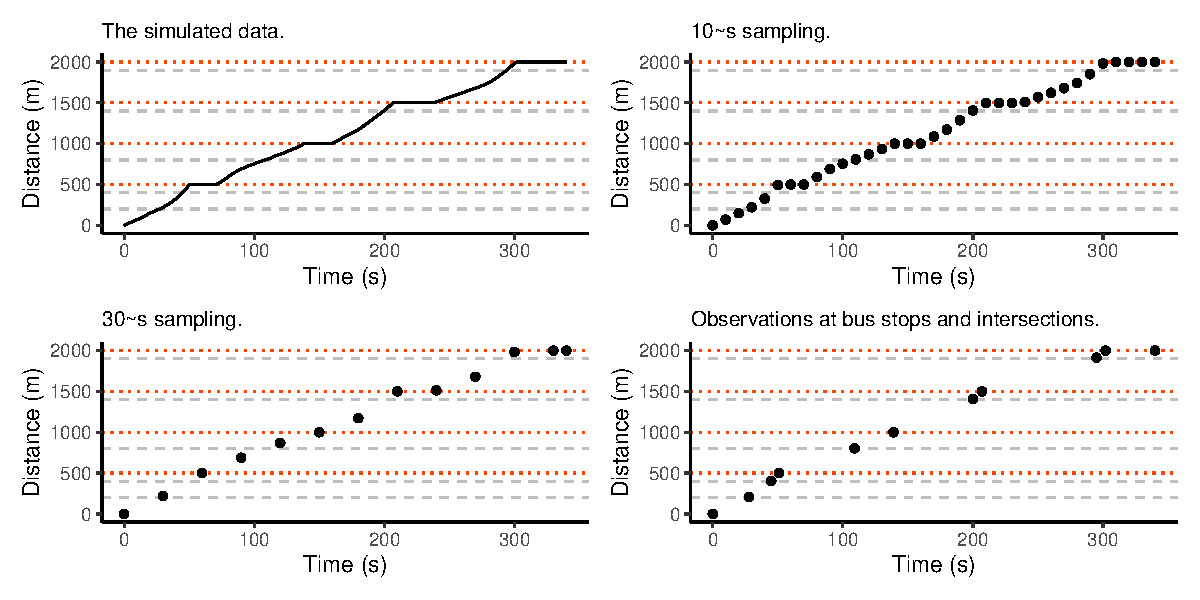
\includegraphics[width=\linewidth]{figure/sim2_graph-1} \caption[Vehicle trajectory with sampled observations for simulation B]{A simulated vehicle trajectory (top left) for simulation B along five road segments (dashed grey lines) with four stops (dotted orange lines). Observations are sampled using three techniques (see text).}\label{fig:sim2_graph}
\end{figure}


\end{knitrout}

\begin{knitrout}\small
\definecolor{shadecolor}{rgb}{0.969, 0.969, 0.969}\color{fgcolor}\begin{figure}[p]
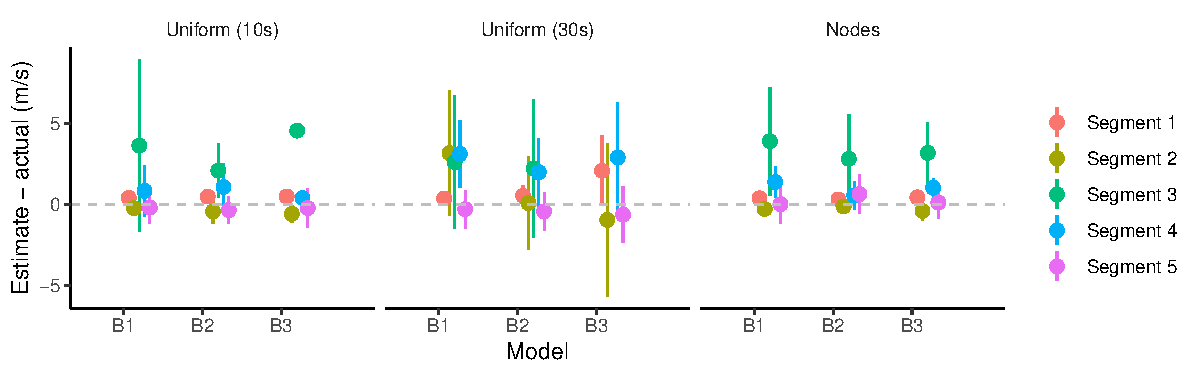
\includegraphics[width=\linewidth]{figure/sim2_pf-1} \caption[Results for simulation B]{Simulation B results for the three models (B1, B2, B3) applied to the data from three sampling methods using $\Np=2000$ particles. Shown is the travel time prediction error along with its standard deviation.}\label{fig:sim2_pf}
\end{figure}


\end{knitrout}





\begin{knitrout}\small
\definecolor{shadecolor}{rgb}{0.969, 0.969, 0.969}\color{fgcolor}\begin{figure}[p]
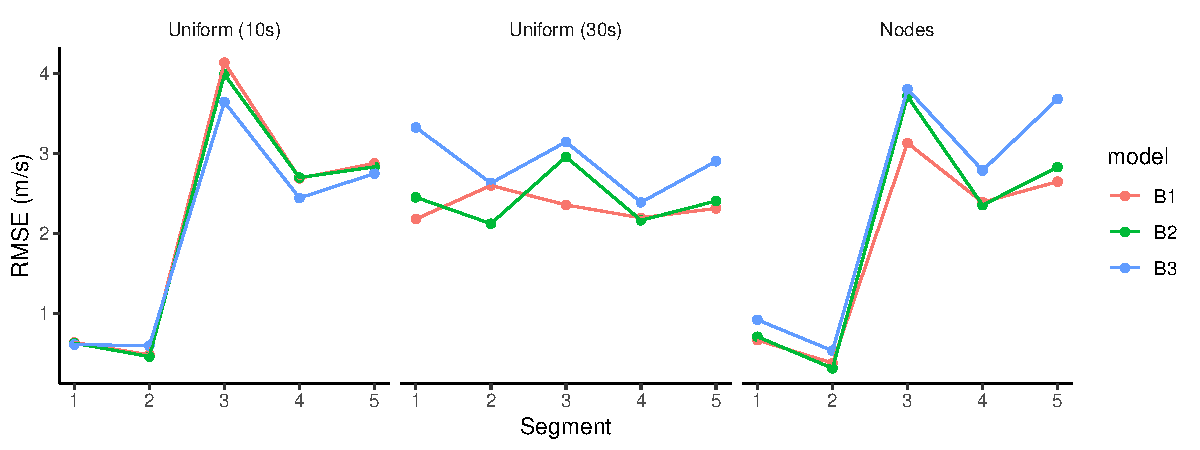
\includegraphics[width=\maxwidth]{figure/sim2_pf_full-1} \caption[Results for simulation B replicated 100~times]{Speed estimation results for 100 simulations. In each the vehicle trajectory was simulated using a different seed and speed estimated by the mean of the particles, which is compared to the true speed using \gls{rmse}.}\label{fig:sim2_pf_full}
\end{figure}

\begin{table}[p]

\caption{\label{tab:sim2_pf_full}RMSE and MAE of average speed estimation for simulation B for three models and three sampling techniques.}
\centering
\fontsize{8}{10}\selectfont
\begin{tabular}[t]{llrr}
\toprule
Sampling method & Model & RMSE (m/s) & MAE (m/s)\\
\midrule
Uniform (10s) & B1 & 2.56 & 1.40\\
 & B2 & 2.51 & 1.35\\
 & B3 & 2.34 & 1.35\\
\midrule
Uniform (30s) & B1 & 2.34 & 1.58\\
 & B2 & 2.43 & 1.63\\
 & B3 & 2.90 & 2.14\\
\midrule
Nodes & B1 & 2.15 & 1.31\\
 & B2 & 2.36 & 1.35\\
 & B3 & 2.70 & 1.57\\
\bottomrule
\end{tabular}
\end{table}


\end{knitrout}





Repeating the simulation 100~times with different vehicle trajectories, we can better compare the models (\cref{fig:sim2_pf_full}). Uncertainties are now much higher, on average, particularly under low-frequency sampling. The models all perform similarly, though B3 has the worst accuracy overall. \Cref{tab:sim2_pf_full} compares the estimates numerically using \gls{rmse} and \gls{mae}, where we see that within each sampling method the errors are similar. Models B1 and B2 perform similarly, while B3 is again consistently worse except under high-frequency sampling.




\phantom{\gls{rmse} \gls{mae}}


\section{Implementing the \rt{} \pf{}}
\label{sec:particle-filter}


The next major step in this work was to implement the model in real-time using C++. Our implementation involves a single call from the R package \verb+transitr+ which commences an infinite loop within C++ which
\begin{enumerate}
\item fetches the lastest observations,
\item attaches them to an existing vehicle, or creates a new one,
\item updates or initialises vehicle states using the particle filter model described in \cref{sec:vehicle_model}, and
\item estimates average road speeds as vehicles traverse the network as described in \cref{sec:vehicle_speeds},
\end{enumerate}
as displayed in \cref{fig:program_flow}. During the process of coding up our implementation (\cref{sec:pf_implementation}), we inevitably ran into issues, some of which are related to computational complexity, while others are due to imperfections with the data (see \cref{sec:pf_issues}). Once the implementation was complete, we needed to estimate the parameters (such as system noise and measurement error) for the model.


In order to assess the \rt{} performance of the model and our \pf{} implementation, we created a virtual \rt{} server which serves historical data. This means we can both process the data faster---we do not need to wait in \rt{} for new observations---and allows us to run the model with different settings and parameter values for comparison. We used (a subset of) data from Tuesday 8~October~2018 for the simulations used in \cref{sec:pf_issues,sec:pf_params}, which were carried out on a virtual machine with 8~Intel Xeon 3.00GHz CPU cores and 32~GB of memory, running Ubuntu 16.04 and R 3.4.1. The results themselves were processed locally using R 3.6.0. These results were published in \citet{Elliott_2020}.





\subsection{C++ particulars}
\label{sec:pf_implementation}

The general construction of the particle filter is straightforward and involves creating \class{Vehicle} and \class{Particle} objects (as well as the \gls{gtfs} objects described in \cref{sec:gtfs}). The \class{Vehicle} objects are stored within an \verb+std::unordered_map+ using their \gls{gtfs} \verb+vehicle_id+ as the key.

When a vehicle is first observed, a new \class{Vehicle} is created and inserted into the map. Then its state is initialised by creating a vector of $\Np$ \class{Particle} objects, each of which is assigned a speed between 0 and 30 m/s, and a distance based on the observation: for GPS observations, map matching is used to determine the approximate location, around which the particles are scattered. In situations where there are multiple candidate locations, particles are distributed uniformly between the minimum and maximum likely distances. For trip updates, the particles are placed at the appropriate stop. When new data for an existing vehicle is observed, the \class{Vehicle}'s relevant properties are updated (such as position and timestamp). Then each \class{Particle} is mutated using the transition function from \cref{sec:vehicle_model} and reweighted according to the likelihood function (\cref{sec:pf-likelihood}). If the effective sample size drops below the threshold $\Nthres=\frac{\Np}{4}$, the state is resampled with replacement and particle weights reset to $\frac{1}{\Np}$. See \cref{app:particle-resampling} for details on particle resampling.

Since the vehicles are modelled independently, and they only need to read from the \gls{gtfs} object (not modify it) the vehicle update step is easily parallelised to use $\tilde M$~cores using the \prog{OpenMP} library \citep{OMP}. This enables up to an $\tilde M$-fold increase in the speed of this step.

Once the update is complete, the segment index of all particles is obtained, and the \emph{minimum} is used as the vehicle's \emph{current segment}. If this is greater than it was at the end of the previous iteration, the average speed along all intermediate segments is computed by using \verb+std::accumulate+,
\begin{lstlisting}
double avg_speed = std::accumulate(state.begin (), state.end (), 0.0,
  [](double x, Particle& p) {
    return x + p.weight () * p.segment_speed.at (seg_index);
  });
\end{lstlisting}\pagebreak
along with the variance,
\begin{lstlisting}
double var_speed = std::accumulate(state.begin (), state.end (), 0.0,
  [&avg_speed](double x, Particle& p) {
    return x + p.weight () *
      pow (p.segment_speed.at (seg_index) - avg_speed, 2.0);
  });
\end{lstlisting}
These observations are then passed to the relevant \class{Segment} object which contains a vector of new data (used in chapter 4). The \class{Vehicle} object contains a pointer to its \class{Trip}, which has a list of \class{Segment} objects:\footnote{Note that we must still ensure each pointer exists before proceeding, as mentioned in \cref{sec:rt-implementation}.}
\begin{lstlisting}
trip ()->segments ().at (seg_index)->push_data (avg_speed, var_speed);
\end{lstlisting}

At this point, we have completed the modelling of the vehicle's state and obtained estimates of any available road speed information.

\subsection{Real-time performance of the \pf{}}
\label{sec:pf_issues}



The two components of the model to assess are the iteration timings and the performance of the particle filter itself. That is, does the program run fast enough to be feasible in real-time, and is the model (and its \pf{} implementation) capable of modelling transit vehicles in real-time?


\paragraph{Is the particle filter fast enough?}
At peak hour on a typical weekday morning, there can be in excess of 1000~buses operating in Auckland. This leads to having more than $1000\Np$~particles in memory, each being mutated and reweighted approximately once every 30~seconds or so. By varying $N$, we can control how quickly each set of observations is processed. \Cref{fig:pf_timings} shows the average timings of the vehicle model component of our application, as well as the average time per particle for varying $N$. More particles require more processing power, though there is additional overhead during the \emph{resampling} phase. Limiting the frequency of resampling is therefore necessary to make the program run faster, which is why we use the effective sample size, $\Neff$, described in \cref{sec:pf} on \cpageref{eq:Neff}.


\begin{knitrout}\small
\definecolor{shadecolor}{rgb}{0.969, 0.969, 0.969}\color{fgcolor}\begin{figure}

{\centering 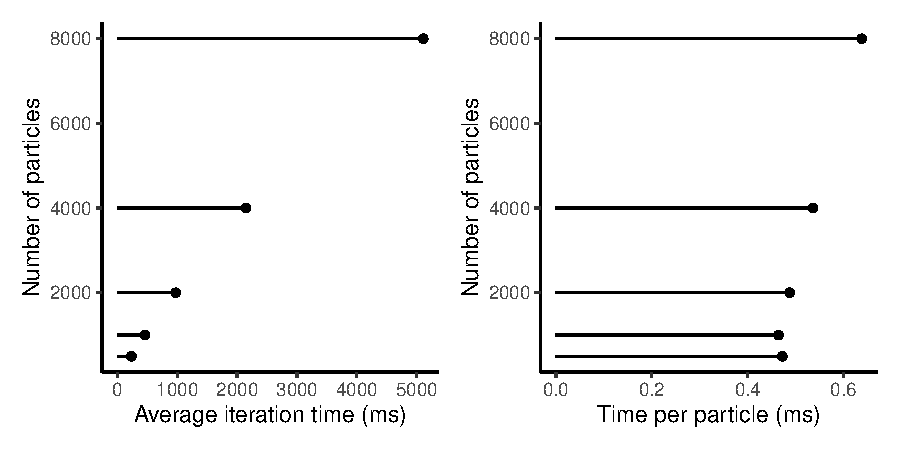
\includegraphics[width=.8\textwidth]{figure/pf_timings-1} 

}

\caption[Timings of the particle filter implemention for varying number of particles]{Timings of the particle filter implemention for varying number of particles. Left: the average iteration time (wall clock). Right: the average time per particle.}\label{fig:pf_timings}
\end{figure}


\end{knitrout}


\paragraph{How does the model perform?}





To assess how well our model performs in real-time, we repeated the simulation with a range of values of system noise $\Vnoise$, \gls{gps} error $\GPSerr$, and the number of particles $\Np$. For each simulation, we computed \emph{proportional effective sample size}, \emph{degeneration rate}, and \emph{relative variance}.

The \emph{proportional effective sample size} is the effective sample size relative to $N$, $\tilde N_\text{eff} = \frac{\Neff}{\Np}$. The higher this value, the less often the vehicle's state needs resampling, decreasing the average iteration time. \Cref{fig:model_performance_neff} shows the effect of $\Np$, system noise, and \gls{gps} error on $\tilde N_\text{eff}$. The most striking relationship is between $\tilde N_\text{eff}$ and \gls{gps} error: for larger error, more particles retain a high likelihood, and so the total weight is more evenly distributed. Conversely, larger values of system noise result in more variation between particles, leading to fewer particles ending near the observation position and decreasing $\tilde N_\text{eff}$.

\begin{knitrout}\small
\definecolor{shadecolor}{rgb}{0.969, 0.969, 0.969}\color{fgcolor}\begin{figure}

{\centering 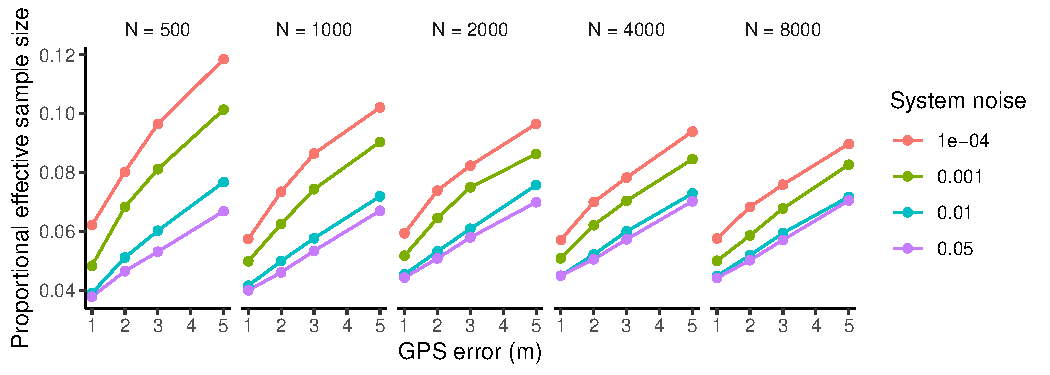
\includegraphics[width=\textwidth]{figure/model_performance_neff-1} 

}

\caption[Proportional effective sample size for varying values of GPS error, system noise, and number of particles]{Proportional effective sample size for varying values of GPS error, system noise, and number of particles.}\label{fig:model_performance_neff}
\end{figure}


\end{knitrout}


The \emph{degeneration rate} is the proportion of samples in which no particles end near the vehicle's reported position. In this case, all the particle likelihoods tend to zero, so the weights become undefined, resulting in the need to reinitialise the vehicle's state which results in the loss of any vehicle speed information along the most recently travelled road segment(s). We see from \cref{fig:model_performance_degen} that increasing \gls{gps} error or the number of particles reduces degeneration rate while increasing system noise shows a negligible reduction in degeneration rate. Larger \gls{gps} error means that particles do not need to end as close to the observed location to have a positive likelihood while increasing $\Np$ means more chance for a particle to end near the true bus.

\begin{knitrout}\small
\definecolor{shadecolor}{rgb}{0.969, 0.969, 0.969}\color{fgcolor}\begin{figure}

{\centering 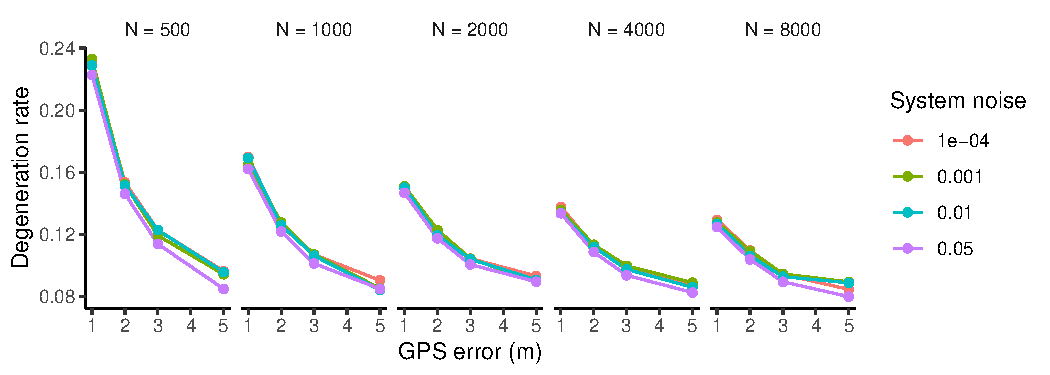
\includegraphics[width=\textwidth]{figure/model_performance_degen-1} 

}

\caption[Degeneration rate for varying values of GPS error, system noise, and number of particles]{Degeneration rate for varying values of GPS error, system noise, and number of particles.}\label{fig:model_performance_degen}
\end{figure}


\end{knitrout}

Finally, we have \emph{relative speed variance} along roads, which we use to compare the precision of the various models. It is the ratio of variance for a single simulation compared to the overall variance for all simulations. Let $\vec z_\ell^{e,s}$ be a vector of all vehicle speeds along road segment $\ell$ during the simulation with \gls{gps} error and system noise equal to $e$ and $s$, respectively. The ratio of the variance of speed for the single simulation compared to all simulations along one single road segment is given by
\begin{equation}
\label{eq:rel_speed_var_ratio}
v_\ell^{e,s} =
\frac{
    \mathrm{Var}(\vec z_\ell^{e,s})
}{
    \mathrm{Var}(\cup_e\cup_s \vec z_\ell^{e,s})
}.
\end{equation}
That is, for each segment in each simulation, we have a value representing whether this simulation estimates speed more or less accurately. We then compute the average ratio for all $L$ road segments,
\begin{equation}
\label{eq:rel_speed_var}
\bar v^{e,s} = \frac{1}{L} \sum_{\ell=1}^L v_\ell^{e,s}.
\end{equation}
A small value of $\bar v^{e,s}$ tells us that, on average, the simulation with \gls{gps} error $e$ and system noise $s$ estimates road speed \emph{with greater precision} than the other simulations. \Cref{fig:model_performance_var} presents these results, where we see the greatest effect on relative variance caused by increasing \gls{gps} error. Increasing $\Np$ produces a small decrease, and changes to system noise show no discernible effect.


\begin{knitrout}\small
\definecolor{shadecolor}{rgb}{0.969, 0.969, 0.969}\color{fgcolor}\begin{figure}

{\centering 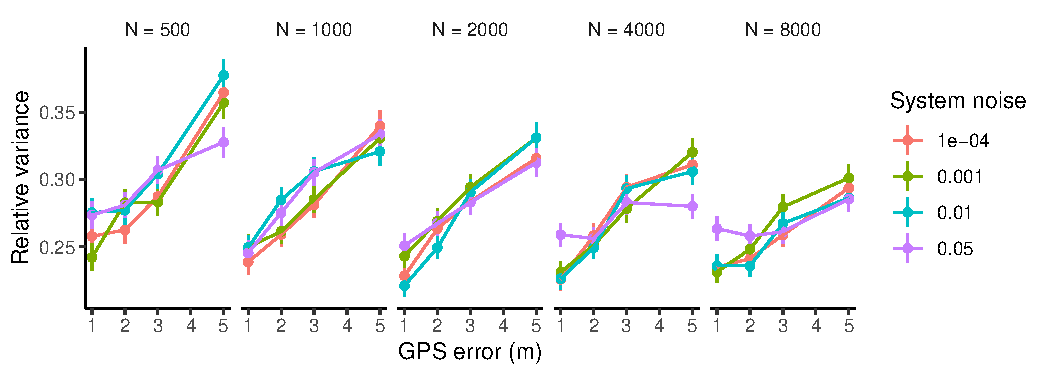
\includegraphics[width=\textwidth]{figure/model_performance_var-1} 

}

\caption[Relative speed variance for varying values of GPS error, system noise, and number of particles]{Relative speed variance for varying values of GPS error, system noise, and number of particles.}\label{fig:model_performance_var}
\end{figure}


\end{knitrout}


The results displayed in \cref{fig:model_performance_neff,fig:model_performance_degen,fig:model_performance_var} present a \emph{trade-off} between performance and estimation. Increasing \gls{gps} error increases the effective sample size, which reduces the frequency of resampling and speeds up each iteration. We also see a reduction in the rate of degeneration, which implies the particle filter is less likely to lose the vehicle and provide the desired speed estimates. However, increasing \gls{gps} error also increases the relative uncertainty of speed estimates. Increasing the number of particles generally results in a reduction in both degeneration rate and relative uncertainty, but, from \cref{fig:pf_timings}, this comes at the cost of increased computational demand.

\subsection{Handling invalid data in real-time}
\label{sec:data_issues}

Much of the degeneration or \emph{vehicle loss} can be attributed to irregularities with the incoming real-time data. There are two leading causes of this, described below, which can be detected and potentially avoided with a similar solution.


\paragraph{Buses that appear to go backwards}

One of the prominent assumptions of our model is that the bus cannot go backwards along the route, which is implemented by only allowing for non-negative values of speed. However, a couple of scenarios can lead to the \emph{appearance} of a reversing bus, both of which are related to \emph{\gls{gps} waypoints}; that is, the \gls{avl} systems in Auckland Transport's buses are programmed to not only report their position periodically but also to report their arrival at certain waypoints. These can include bus stops (which result in an arrival or departure time update) as well as some major intersections. The issue is that, rather than reporting the bus's \gls{gps} position, they report the \gls{gps} coordinates of the waypoint itself. This is often acceptable since the bus continues straight past the intersection or bus stop before reporting another position. However, if there is congestion leading into the waypoint, the bus may:
\begin{enumerate}[i.]
\item approach the waypoint, decide it has arrived, and report its position \emph{at the waypoint},
\item get stopped in a queue for some time,
\item decide it is time for another position update, based on its GPS position.
\end{enumerate}
\Cref{fig:bus_going_backwards} presents an example of this.

\begin{knitrout}\small
\definecolor{shadecolor}{rgb}{0.969, 0.969, 0.969}\color{fgcolor}\begin{figure}

{\centering 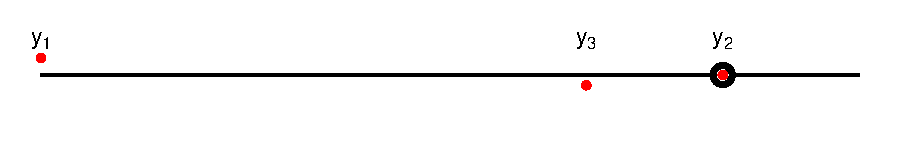
\includegraphics[width=.8\textwidth]{figure/bus_going_backwards-1} 

}

\caption[Visual demonstration of the ``reversing bus'' phenomenon]{Three sequential observations of a vehicle approaching an intersection (hollow circle). When the bus nears the intersection, it reports its position exactly at the intersection ($\Vobs_2$); however, there is a queue at this intersection, so the next observation ($\Vobs_3$) is behind the previous one, demonstrating the ``reversing bus'' phenomenon.}\label{fig:bus_going_backwards}
\end{figure}


\end{knitrout}


The effect this has on the \pf{} is that, after observing $\Vobs_2$, the vehicle's state (represented by a sample of particles) will all be around the intersection. On receiving the next observation $\Vobs_3$, the particles are transitioned \emph{forward} by $(\Vtime_3 - \Vtime_2)$~seconds, which places them at or beyond the intersection; none of the particles will be near observation $\Vobs_3$ and will likely all have a likelihood of zero. In this case, the particle filter has degenerated and needs reinitialising.


A similar situation occurs when approaching a bus stop that has an intersection just before it. Here, the bus gets stopped at the intersection, but not before reporting its position at the stop since it was almost there. A subsequent observation then shows the bus at the intersection, which again appears to involve a reversing bus. The main issue we face is that \emph{we do not know the location of intersections} since there is no easily accessible data for this.\footnote{We presented an intersection model, but this was more of a demonstration of flexibility, not of functionality.}


Checking for the bus-reversing scenario in real-time requires mapping of observations onto the route shape; that is, the \emph{inverse measurement function}, allowing us to detect if the bus has gone backwards:
\begin{equation}
\label{eq:vehicle_rev_check}
\Vmeas^{-1}(\Vobs_k) < \Vmeas^{-1}(\Vobs_{k-1}).
\end{equation}
Of course, the inverse function is not exact, since the true location is unlikely to be positioned exactly on the line (roads have width, and \gls{gps} devices have error). To compute $\Vmeas^{-1}$, we find the shortest distance along the route's shape that is closer than a threshold of $3\GPSerr$, which allows for situations where the route passes the observed location point more than once (such as in loops).

If the observation is determined to be going backwards, we have to decide between
\begin{enumerate}[i.]
\item ignoring the current observation, or
\item ignoring the previous observation and restoring the vehicle's previous state.
\end{enumerate}
If we can determine that the first observation is a pre-emptive observation (that is, at a waypoint), then option (ii) is the logical choice, although this requires storing each vehicle's state \emph{twice}. Otherwise, it is easier to ignore the current observation completely and use option (i). Note that, were intersection locations knowable, we could include this behaviour in the model; as it stands, however, this workaround is required to avoid unnecessary degeneration.


\paragraph{Buses that remain stationary}

Another situation (which can also occur around unknown intersections) is when the bus does not move between successive observations (or it moves very slowly). For example, the bus may need to turn onto a major road, for which there is a queue of traffic. The bus will report its position when it arrives, and may again report its position after moving a few meters. If our model does not allow for the bus to suddenly slow down in these situations, the particles will all be far ahead of the bus and degeneration will occur.


We can determine if the bus has remained more-or-less stationary by computing the distance between successive observations and comparing to a threshold:
\begin{equation}
\label{eq:vehicle_dist_check}
\dist{\Vobs_{k-1}, \Vobs_k} < \distThreshold =
\Vtdiff_k \min_i\left(\Vspeed_k\vi\right).
\end{equation}
The threshold here is the expected distance travelled in $\Vtdiff_k$~seconds by the slowest particle. Rather than slowing the particles (which could run into the opposite problem once the vehicle passes through the intersection), we sample a temporary speed,
\begin{equation}
\label{eq:vehicle_temp_speed}
\Vspeed_k\vi \sim
\Uniform{0}{\frac{\dist{\Vobs_{k-1}, \Vobs_k}}{\Vtdiff_k}},
\end{equation}
which is used for one single iteration.

Again, if we knew the locations of intersections, we could integrate this behaviour into the model. Particles could partake in ``creeping'' up to the intersection, before quickly accelerating back up to speed on the next road segment. Even then, however, the above behaviour would still need to be included to handle non-intersection related slowing down, for example, when reaching a congested section of a road.

\subsection{Parameter selection}
\label{sec:pf_params}

Once the inherent data issues have been dealt with,
we can begin determining the values of the model parameters.
Some of these are fixed and constant across all vehicles, routes, and stops,
for example,
GPS error, $\GPSerr$,
system noise, $\Vnoise$,
and minimum dwell time, $\mindwell$.
Others will inevitably vary between routes, stops, and time of day,
such as stopping probability, $\Prstop$,
and dwell time, $\dwell$.


% We explore these by modelling a subset of routes throughout Auckland over several days,
% using historical data to allow us to vary parameters and compare their effects.
% Some parameters, notably $\GPSerr$ and $\dwell$
% can be determined from the data:
% the value $\GPSerr$ can be approximated by looking at the variability
% of points around the route,
% since we assume there is no directional bias,
% so the distance from an observation to the route is an approximate estimate
% of measurement error.


\subsubsection{GPS error}
\label{sec:pf_params_gps}

The GPS or \emph{measurement} error used in the model has a strong effect on performance, as we saw in \cref{sec:pf_issues}. We can get a simple estimate of GPS error by examining the distribution of observations around the route; that is, we computed the shortest distance between the route and each observation, and graphed the results in \cref{fig:pf_param_gps}. We see two modes at about 0.5 and 2.5~meters, which could be due to a multitude of reasons. One likely one, however, is \emph{road width}, since the route shapes typically run in the middle of the road and the buses drive either side of the center line. Single-lane roads will have a smaller average distance between the bus and the center line, while for roads with two or more lanes, this will be larger. Additionally, some roads have a median (either painted or raised) which further increases the distance between the bus and the ``center line''. It is possible that some combination of this could result in the distribution shown in \cref{fig:pf_param_gps}.



\begin{knitrout}\small
\definecolor{shadecolor}{rgb}{0.969, 0.969, 0.969}\color{fgcolor}\begin{figure}
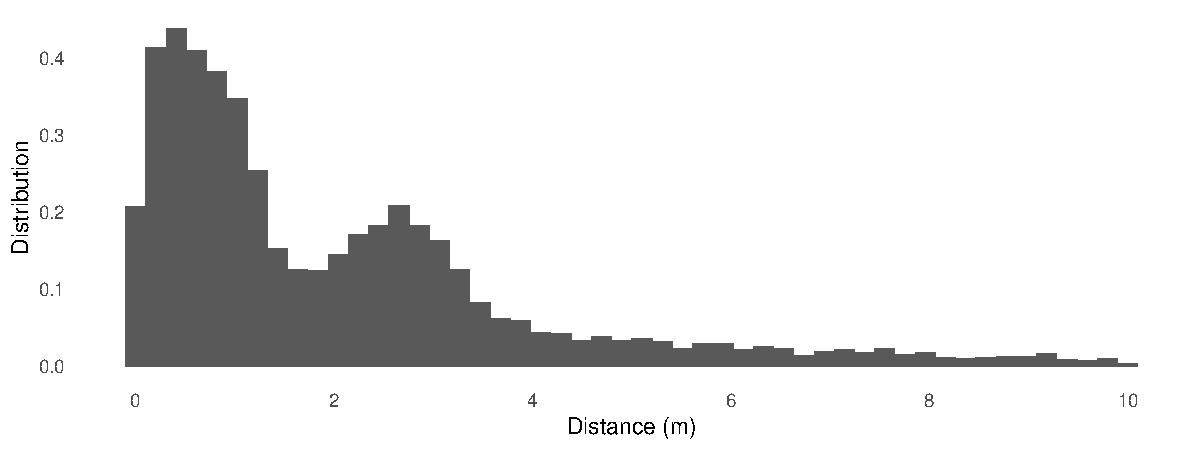
\includegraphics[width=\maxwidth]{figure/pf_param_gps-1} \caption[Distribution of distance from observation to nearest point on the route, truncated to 10~m]{Distribution of distance from observation to nearest point on the route, truncated to 10~m.}\label{fig:pf_param_gps}
\end{figure}


\end{knitrout}

The other issue is the heavy tail in the distribution of distance to path, which we trunctated to 10~meters to more easily see the modes. GPS devices usually have good accuracy, but occasionally they may be quite far off of the true location, possibly due to physical interference. 6\% of bus observations were more than 10~meters from the shape, excluding any observations greater than 50~meters since these were most likely attributed to the wrong trip (and therefore not anywhere near the route path). This would explain a large proportion of the degeneration rate (\cref{fig:model_performance_degen}), which we saw previously decreases significantly with increased GPS error.





\subsubsection{System noise}
\label{sec:pf_params_noise}

The definition of system noise is model-dependent; for transition models $f_{A1}$ and $f_{A2}$ it is \emph{the average change in speed per second}, while for model $f_{A3}$ it is \emph{the average change in acceleration per second}. From the simulations in \cref{sec:pf_issues}, we demonstrated that system noise affected the performance of the particle filter (how often resampling is required) but neither the degeneration rate nor parameter estimation.

Unlike GPS error, it is not possible to estimate system noise directly from the data. Indeed, most of the time a vehicle's speed is constant, but may change suddenly at certain locations (which are unknown), so the system noise must allow for this. We found that a smaller value of system noise under the second transition model $f_{A2}$ gave the best results in terms of sampling possible trajectories, and as such this was the model used during the simulation.



\subsubsection{Dwell times}
\label{sec:pf_params_dwell}

We are able to observe a large proportion of dwell times at stops, by compiling all those for which we have observed both arrival times $\Varr_{srm}$ and departure times $\Vdep_{srm}$ at stop $m$ of trip $r$ on day $s$ giving us a set of dwell times
\begin{equation}
\label{eq:dwell_time_obs}
\Vdwell_{srm} = \Vdep_{srm} - \Varr_{srm}
\end{equation}

\begin{knitrout}\small
\definecolor{shadecolor}{rgb}{0.969, 0.969, 0.969}\color{fgcolor}\begin{figure}
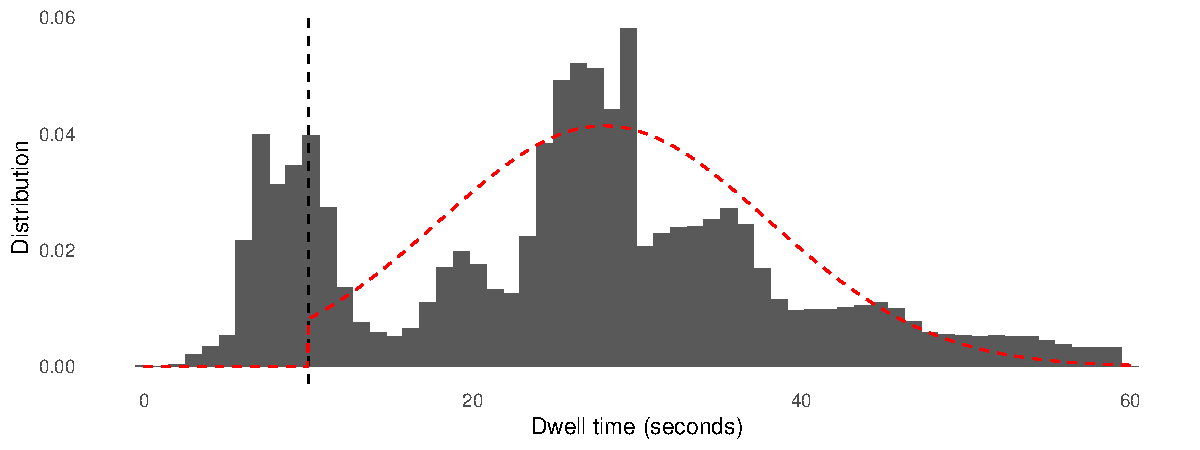
\includegraphics[width=\maxwidth]{figure/observed_dwell-1} \caption[Distribution of dwell times observed over the course of five days, truncated at one minute]{Distribution of dwell times observed over the course of five days, truncated at one minute.}\label{fig:observed_dwell}
\end{figure}


\end{knitrout}

There is no precise way to measure the minimum dwell time parameter $mindwell$. \cite{Hans_2015} used $\mindwell = 6$~seconds, which is marked by a dashed vertical line in \cref{fig:observed_dwell}. There are a few dwell times less than this, but given the spike at 6~seconds, it seems reasonable to continue with this value.

The raw data from five~days' observations are shown in \cref{fig:observed_dwell}. Here, we see an interesting pattern with apparent peaks every nine~seconds. While we could not determine the precise cause, we assume it to be due to a systematic problem in the arrival time recording system used to collect the data. From the historical dwell time data, we were able to estimate the mean and variance of dwell time for each stop $j$, $\bar\dwell_j$ and $\dwellvar_j$, respectively, which could then be used in the dwell time model.


The dwell times for each stop calcualted above \emph{include} the minimum dwell time phase. To avoid having to recompute each stop's dwell time parameter whenever $\mindwell$ is changed, we adjusted the mean of each stop's dwell time at run time to account for the minimum dwell time. That is, we use $\dwell_j = \bar\dwell_j - \mindwell$ in \cref{eq:stop_dwell_time}.



\chapter{Transit network}
\label{cha:network_model}

\phantom{\gls{gtfs},\gls{gtfs},\gls{gtfs}}

The collection of bus stops and intersections, and the roads which connect them, we refer to as a \emph{transit network}. The \emph{state} of this network changes in response to events throughout the city, some of which are predictable---peak traffic, for example---while others are not, such as accidents or weather events. In \cref{cha:vehicle_model}, we measured this state by tracking individual vehicles as they moved through the network. Now we discuss the network state itself, how it changes over time, and how we use the speed observations to update its state. Finally, we discuss short-term forecasting as could be used for arrival time estimation in \cref{cha:prediction}.


Estimation of the network's state from vehicle travel time observations requires an understanding of the relationship between them. The underlying state of the network determines how fast (or slow) vehicles travel through it, which changes over time. Since speed is unlikely to be constant over segments, we use \emph{average speed} over the length of a segment, calculated using the length of the segment and how long vehicles take to travel along it,
\begin{equation}
\label{eq:ch4:average_speed_formula}
\text{average speed (m/s)} = \frac{
\text{segment length (m)}
}{
\text{travel time along segment (s)}
}.
\end{equation}
However, there are a variety of factors that may affect the average speed of individual buses, such as driver behaviour, cyclists sharing the road, variance between lanes, or pedestrians crossing the road, to name a few. Thus, even buses travelling along a road at the same time often have different (average) speeds, resulting in a \emph{distribution} of vehicle speeds, as demonstrated in the top half of \cref{fig:nw_model_hierarchy}. To further complicate matters, the observed average vehicle speeds are made with a level of uncertainty, which is depicted in the second half of \cref{fig:nw_model_hierarchy}.


Previous work has used \emph{travel time} to model the network state \citep{Yu_2011,Cats_2015,Gong_2013,Shalaby_2004,Reinhoudt_1997}, while others have used \emph{vehicle speed}, as I introduced above \citep{Ma_2019,Celan_2017,Celan_2018,Xinghao_2013}. We found that travel times tended to have long tails which the \kf{} was less capable of modelling, and required a lot of manual work determining the appropriate parameter values. Speed, however, is independent of road length, so most of the parameter values could take a single value across all segments.


In \cref{sec:nw_model}, we develop a model to estimate the distribution of vehicle speeds along roads throughout the transit network. In \cref{sec:nw_realtime}, I describe the real-time implementation of the model, while \cref{sec:nw_par_est} considers the estimation of model parameters from historical data. The model's forecasting ability can also be improved with historical data, as we discuss in \cref{sec:nw_hist_model} and revisit in \cref{cha:prediction}. Finally, we examine the computational aspects of the model's real-time implementation and its feasibility in \cref{sec:nw_implementation}. As with the vehicle model, we must keep in mind the real-time nature of the application, so computational efficiency is an important consideration throughout.


\begin{knitrout}\small
\definecolor{shadecolor}{rgb}{0.969, 0.969, 0.969}\color{fgcolor}\begin{figure}

{\centering 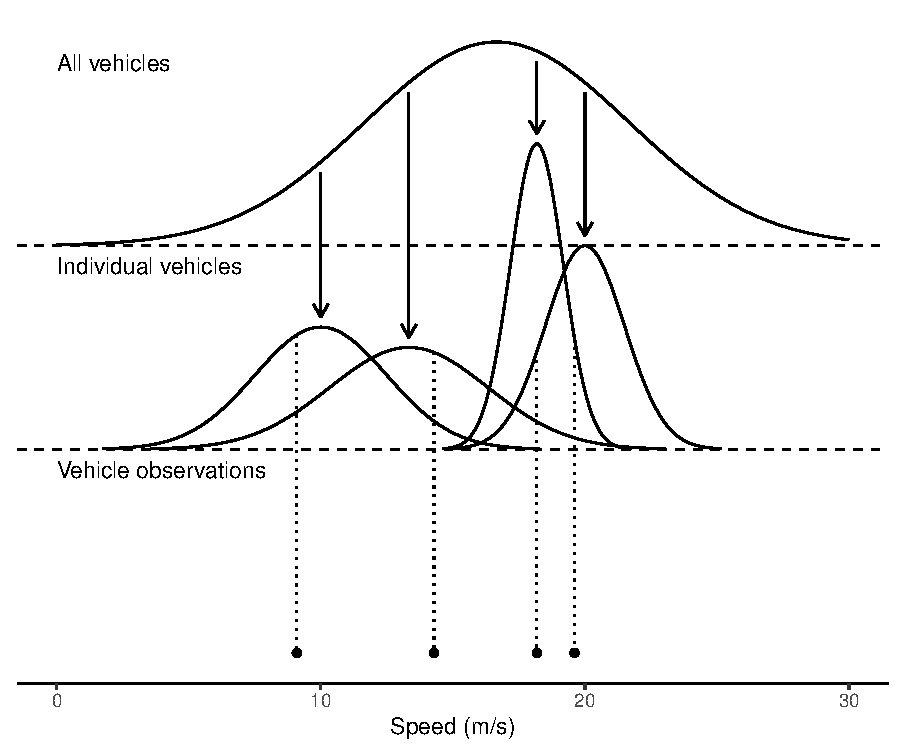
\includegraphics[width=0.6\textwidth]{figure/nw_model_hierarchy-1} 

}

\caption[The hierarchy of speed uncertainty along a single road segment]{The hierarchy of speed uncertainty along a single road segment is composed of \emph{between-vehicle variability} and \emph{measurement error}. The top curve shows the underlying distribution of average vehicle speeds with solid arrows representing the true average speed of four vehicles. The second level shows the measurement uncertainty for each vehicle with the observed values represented as dots at the bottom of the graph.}\label{fig:nw_model_hierarchy}
\end{figure}


\end{knitrout}

\section{A model of average road speed}
\label{sec:nw_model}


The relationship between the underlying road speed and the value observed in \cref{cha:vehicle_model} involves two steps. The first is the relationship between the average traffic speed and the vehicle's true average speed. Second is the relationship between \emph{actual} and \emph{observed} (or, more specifically, estimated) average speed. This type of model is referred to as a \emph{hierarchical (Bayesian) model}, as demonstrated graphically in \cref{fig:nw_model_hierarchy}.


Let us first consider the state of the network at time $t_c$, which we denote
\begin{equation}\label{eq:nw_state}
\boldsymbol{\NWstate}_c =
\left[\NWstate_{1,c}\ \cdots\ \NWstate_{L,c}\right]^\top,
\end{equation}
a vector containing the current real-time average traffic speed along all $L$ roads in the network. However, modelling the full state would increase computational demand as $L$ gets large, so we consider each road segment $\ell$ \emph{independently} (this assumption is revisited in \cref{sec:kf-limits}).


Vehicles travelling along road segment $\ell$ at time $t_c$ have an underlying average speed of $\NWstate_{\ellc}$~seconds, which changes with an average rate of $\NWnoise_\ell$ m/s$^2$. Assuming the underlying road state is a Markov process, the model for the evolution of traffic speed along a road with a maximum velocity (speed) of $\MaxSpeed_\ell$~\gls{mps} is
\begin{equation}\label{eq:nw_state_markov}
\NWstate_{\ellc} \sim
\TNormal{\mathcal{F}_c(\NWstate_{\ellc-1})}{(\NWtdiff_c \NWnoise_c)^2}{0}{\MaxSpeed_\ell},
\end{equation}
where $\NWtdiff_c = t_c - t_{c-1}$ is the time since the last update. This model allows traffic speed to follow temporal trends through the time-dependent transition function $\mathcal{F}_c$ (peak hour traffic, for example) as well as react to real-time events, such as accidents or weather events.


As already mentioned, there are many factors which can affect the speed of a vehicle along a given road segment. To encapsulate this uncertainty, we introduce a single parameter $\NWvar_{\ellc}$, which describes the \emph{between-vehicle variability}, or the width of the distribution at the top of \cref{fig:nw_model_hierarchy}. The true average speed of bus $m$ along road segment $\ell$ at time $t_c$ is denoted $\Vtt_{\ellc}^m$, and is assumed to be an observation from the population distribution with mean $\NWstate_{\ellc}$ and variance $\NWvar_{\ellc}^2$, again truncated appropriately:
\begin{equation}\label{eq:nw_vehicle_tt}
\Vtt_{\ellc}^m \sim
\TNormal{\NWstate_{\ellc}}{\NWvar_{\ellc}^2}{0}{\MaxSpeed_\ell}.
\end{equation}


Once a vehicle has traversed a segment, we estimate its average speed as $\Vttobs_{\ellc}^m$, as estimated in \cref{eq:pf_travel_time_mean} on \cpageref{eq:pf_travel_time_mean}. We assume the measurement is made with uncertainty $\Vtterr_{\ellc}^m$, as demonstrated in \cref{fig:nw_model_hierarchy} as the second level of the hierarchy, which is expressed as
\begin{equation}\label{eq:nw_tt_obs_dist}
\Vttobs_{\ellc}^m \sim \Normal{\Vtt_{\ellc}^m}{(\Vtterr_{\ellc}^m)^2}.
\end{equation}



To assess the model, we performed a simulation where all the parameter values are known (based off of the values estimated in \cref{sec:nw_par_est}). \Cref{fig:nw_sim_data} shows the three stages of the model hierarchy.


\begin{knitrout}\small
\definecolor{shadecolor}{rgb}{0.969, 0.969, 0.969}\color{fgcolor}\begin{figure}

{\centering \subfloat[Underlying average vehicle speed\label{fig:nw_sim_data1}]{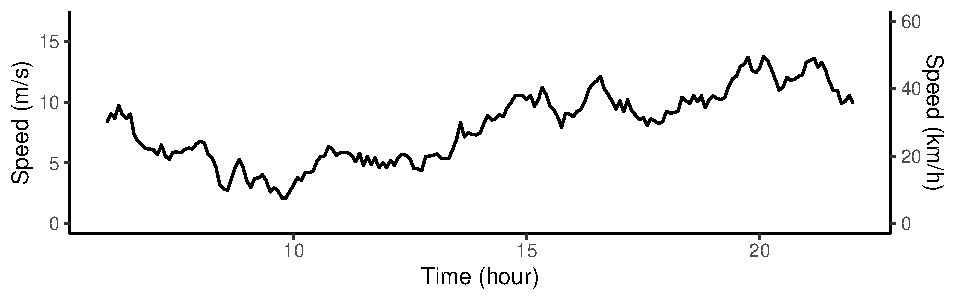
\includegraphics[width=0.8\textwidth]{figure/nw_sim_data-1} }\\
\subfloat[Actual bus speeds (averaged over road segment)\label{fig:nw_sim_data2}]{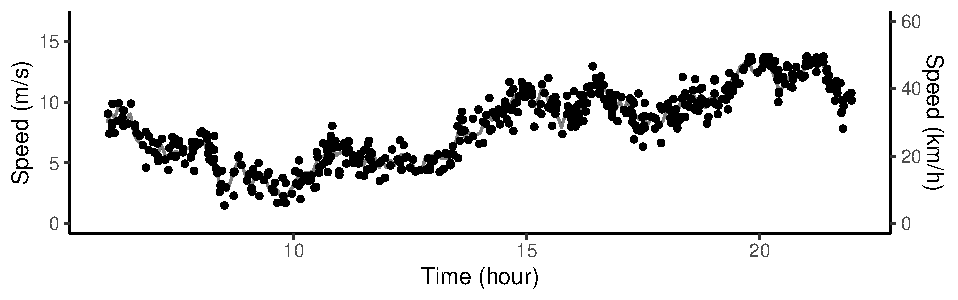
\includegraphics[width=0.8\textwidth]{figure/nw_sim_data-2} }\\
\subfloat[Observed average bus speeds, with vertial lines representing measurement error.\label{fig:nw_sim_data3}]{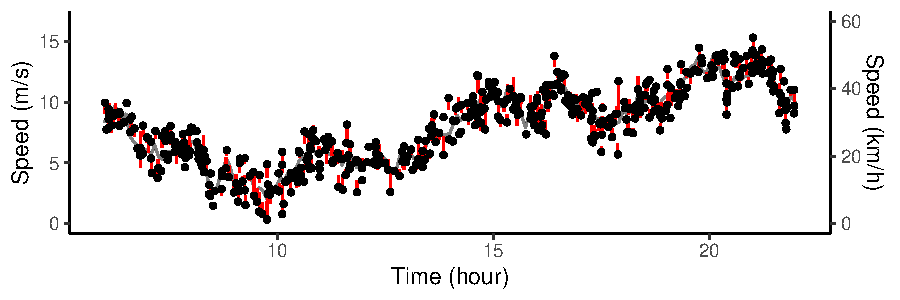
\includegraphics[width=0.8\textwidth]{figure/nw_sim_data-3} }\\

}

\caption[Simulated data showing average vehicle speed along a road]{Simulated data showing average vehicle speed along a road. The right hand axis is shown as a guide for readers not familiar with speeds measured in meters per second.}\label{fig:nw_sim_data}
\end{figure}


\end{knitrout}


Observed vehicle speeds for a real segment, displayed in \cref{fig:tt_figure}, shows some similarities to the simulated data, with one notable difference: the peak-hour spike. This spike is due, in part, to the location of the road, the Symonds Street overbridge:\footnote{Since a lot of traffic arriving into the CBD from the south must use this bridge, it can get very congested.} there is often a (very long) queue of buses from many routes converging there on the central city. In this section, we use the simulated data to evaluate the model under ``nice'' conditions and then test it on this real data to see how well the model copes with these types of phenomenon. The map in \cref{fig:nw_seg_maps} on \cpageref{fig:nw_seg_maps} shows the location of this and several other road segments.


\begin{knitrout}\small
\definecolor{shadecolor}{rgb}{0.969, 0.969, 0.969}\color{fgcolor}\begin{figure}

{\centering 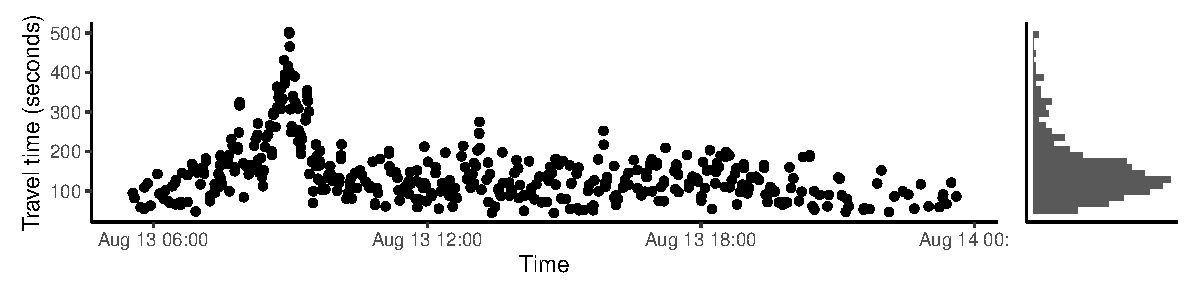
\includegraphics[width=0.8\linewidth]{figure/tt_figure-1} 

}

\caption[Road state observations along a single road segment.]{Road state observations along a single road segment over time, comparing travel time (top) to speed (bottom).}\label{fig:tt_figure}
\end{figure}


\end{knitrout}

\section{Real-time network model}
\label{sec:nw_realtime}

Due to the time constraints of real-time applications, our framework uses a Kalman filter to implement the model described above, which, as previously discussed, is a highly efficient estimation method. This requires the transition and measurement matrices as described in \cref{sec:kf} on \cpageref{sec:kf}. The measurement matrix is the identity matrix $\mat{I}$ since the data are now direct observations of the underlying state (average vehicle speed):
\begin{equation}
\label{eq:kf_meas_identity}
\NWstate_{\ellc} = \mat{H}\Vtt_{\ellc} + w_{\ellc} = \Vtt_{\ellc} + w_{\ellc}
\end{equation}
We also use the identity matrix for the transition matrix $\mat{F}$ as our best guess of the current traffic state is the previous state. So, assuming that $\NWvar_{\ell}$ and $\NWnoise_{\ell}$ are known, for now, we have everything needed to implement a Kalman filter on $\NWstate_{\ellc}$.


\subsection{Predict step}
\label{sec:kf_predict}

In the examples presented, we use a stationary transition function, that is, $\mat{F}_c = 1$, which implies an assumption that traffic speed is constant over short periods (less than five~minutes). The vector of all segment speed observations up to and including time $t_{c}$ is defined as
\begin{equation}\label{eq:all_seg_obs}
\NWobs_{\ell,1:c}^{\boldsymbol{\cdot}} = \bigcup_{t=1}^{c} \bigcup_{v\in V_{\ell,t}} \NWobs_{\ell,t}^v,
\end{equation}
where $V_{\ellc}$ is the set of all vehicles traversing segment $\ell$ at time $t_c$. Then the estimated segment state, conditional on all observations up to time $t_{c-1}$, has mean
\begin{equation}\label{eq:ch4:nw_state_mean_est}
\hat\NWstate_{\ellc|c-1} =
    \E{\NWstate_{\ellc} \cond{} \NWobs_{\ell,1:c-1}^{\boldsymbol{\cdot}}}
\end{equation}
and variance
\begin{equation}\label{eq:ch4:nw_state_var_est}
\NWstatevar_{\ellc|c-1} =
    \Var{\NWstate_{\ellc} \cond{} \NWobs_{\ell,1:c-1}^{\boldsymbol{\cdot}}},
\end{equation}
which are predicted using the following equations:
\begin{equation}
\label{eq:nw_kf_predict}
\begin{split}
\hat\NWstate_{\ellc|c-1} &=
    \hat\NWstate_{
\ellc-1|c-1} \\
\NWstatevar_{\ellc|c-1} &= \NWstatevar_{\ellc-1|c-1} + \left(\NWtdiff_c\NWnoise_\ell\right)^2
\end{split}.
\end{equation}
This prediction is shown in \cref{fig:nw_kf1}. Alternatively, were forecast information available, we could use a transition matrix $\mat F_c$ to describe how traffic might change over time, as is shown in \cref{fig:nw_kf2}.


\begin{knitrout}\small
\definecolor{shadecolor}{rgb}{0.969, 0.969, 0.969}\color{fgcolor}\begin{figure}

{\centering \subfloat[Constant speed model. The prediction is equal to the previous state with an increased variance.\label{fig:nw_kf1}]{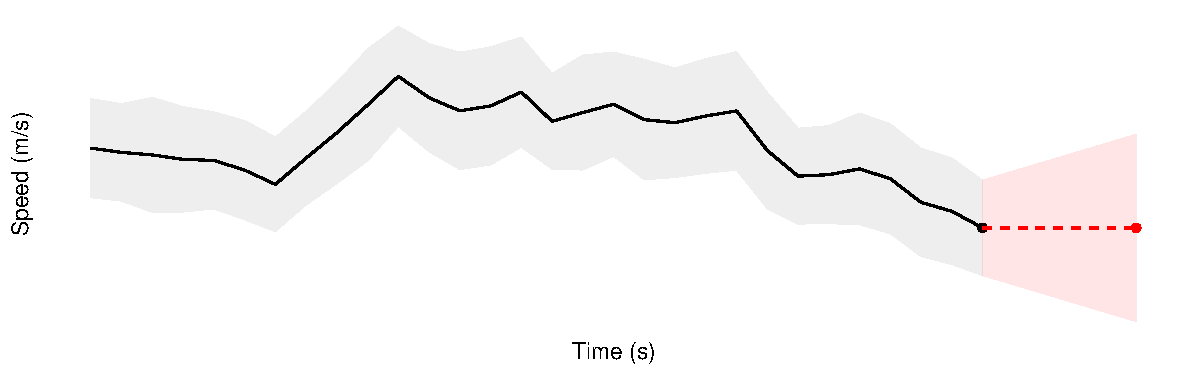
\includegraphics[width=0.8\textwidth]{figure/nw_kf-1} }\\
\subfloat[Historical change based model. The dashed blue line represents historical average speed, which the prediction accounts for under this model.\label{fig:nw_kf2}]{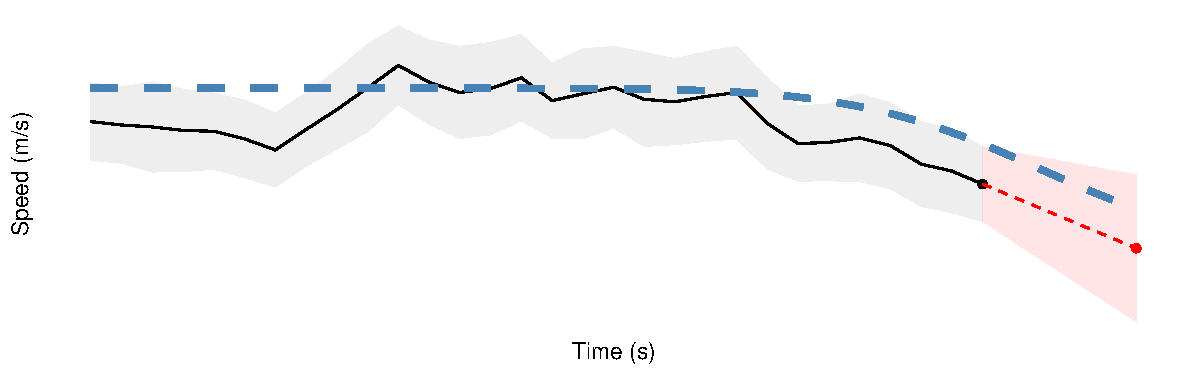
\includegraphics[width=0.8\textwidth]{figure/nw_kf-2} }\\

}

\caption[Network state prediction using constant speed and historical trend models]{Network state prediction depends solely upon the current state (black dot). The mean (solid black line) and uncertainty (shaded grey region) represent previous states. The predicted state has mean (red point) and uncertainty (shared pink region) dependent on the chosen model.}\label{fig:nw_kf}
\end{figure}


\end{knitrout}


\subsection{Update step}
\label{sec:kf_update}

Updating the \kf{} involves taking the predicted state and updating it using \emph{observations} of vehicle speeds along road segments. These are obtained from the \pf{} (\cref{sec:vehicle_speeds}). However, it is possible to have multiple observations per road segment in one update period, as it is common for buses to travel one behind the other, particularly along bus lanes. Therefore, we have a vector of observations passing through segment $\ell$ in the time interval $(t_{c-1}, t_c]$,
\begin{equation} \label{eq:nw_seg_obs}
\NWobss_{\ell c} = \bigcup_{v\in V_{\ell c}} \NWobss_{\ell c}^v,
\end{equation}
which can be the empty set $\NWobss_{\ell c} = \emptyset$ if no vehicles travel through the segment in the interval.


When updating the network, each observation must be accounted for. One way would be to combine the observations into a single estimate; however, this involves averaging observations and uncertainties. An alternative is to use an \emph{\infil{}}, which allows the summation of information from multiple observations \citep{Mutambara_2000}. The information filter involves inverting the state uncertainty $\NWstatevar$; however, this is a simple computation due to having a one-dimensional state---if we were to estimate the state of all segments simultaneously, inverting the $L\times L$ uncertainty matrix would be computationally demanding, or even impossible, and we would be unable to use the approach.



The first step converts the predicted state vector and covariance matrix into information space by inversion of the covariance matrix, leading to the information matrix
\begin{equation}\label{eq:nw_if_inf_matrix}
\NWinfmat_{\ellc|c-1} = \NWstatevar_{\ellc|c-1}^{-1}
\end{equation}
and information vector
\begin{equation}\label{eq:nw_if_inf_vector}
\hat\NWinfvec_{\ellc|c-1} = \NWstatevar_{\ellc|c-1}^{-1} \hat\NWstate_{c|c-1}.
\end{equation}


Converting the observations into information follows the same formula. Note first that the error needs to account for both measurement error and between-vehicle variation, which are assumed Gaussian and independent, so the total variance is their sum. The observation information matrix is
\begin{equation}\label{eq:nw_if_inf_obsmatrix}
\NWobsinfmat_{\ellc}^v = \frac{1}{\NWvar_{\ell}^2 + (\NWerr_{\ellc}^v)^2}
\end{equation}
and the observation information vector is
\begin{equation}\label{eq:nw_if_inf_obsvector}
\hat\NWobsinfvec_{\ellc}^v = \frac{\hat\NWobs_{\ellc}^v}{
    \NWvar_{\ell}^2 + (\NWerr_{\ellc}^v)^2
}.
\end{equation}
Combining these by summation over vehicles yields the complete information matrix and vector for the time period $(t_{c-1},t_c]$, which are, respectively,
\begin{equation}\label{eq:nw_if_obsupdate_matrix}
\NWobsinfmat_{\ellc} = \sum_{v\in V_{\ellc}} \NWobsinfmat_{\ellc}^v
\end{equation}
and
\begin{equation}\label{eq:nw_if_obsupdate_vector}
\NWobsinfvec_{\ellc} = \sum_{v \in V_{\ellc}} \NWobsinfvec_{\ellc}^v.
\end{equation}



The state update is now just a case of adding the observation information in \cref{eq:nw_if_inf_obsmatrix,eq:nw_if_inf_obsvector} to the predicted state information in \cref{eq:nw_if_inf_matrix,eq:nw_if_inf_vector}:
\begin{equation}
\label{eq:nw_if_update}
\begin{split}
\NWinfmat_{\ellc|c} &= \NWinfmat_{\ellc|c-1} + \NWobsinfmat_{\ellc} \\
\hat\NWinfvec_{\ellc|c} &= \hat\NWinfvec_{\ellc|c-1} + \NWobsinfvec_{\ellc}
\end{split}.
\end{equation}
Note that, in situations where no data is observed for a given segment, the information for that segment is zero, so there is no further change to the predicted state value. This could be useful at peak hour, for example, if the transition function predicts changes based on historical trends.


Finally, we back-transform the information into the state space,
\begin{equation}
\label{eq:nw_if_statespace}
\begin{split}
\hat\NWstate_{\ellc|c} &= \NWinfmat_{\ellc|c}^{-1} \hat\NWinfvec_{\ellc|c} \\
\NWstatevar_{\ellc|c} &= \NWinfmat_{\ellc|c}^{-1}
\end{split}.
\end{equation}

The primary constraint on the model is the dependence on $\NWvar_{\ell}$ and $\NWnoise_{\ell}$; however, before considering the estimation of these values, we apply the Kalman filter model to the simulated data in \cref{fig:nw_sim_data} for which the parameter values are known.


\begin{knitrout}\small
\definecolor{shadecolor}{rgb}{0.969, 0.969, 0.969}\color{fgcolor}\begin{figure}

{\centering \subfloat[\kf{} estimate of the state mean (red line) and variance (shaded region) along with the true value (dashed black line).\label{fig:nw_simdata_fit1}]{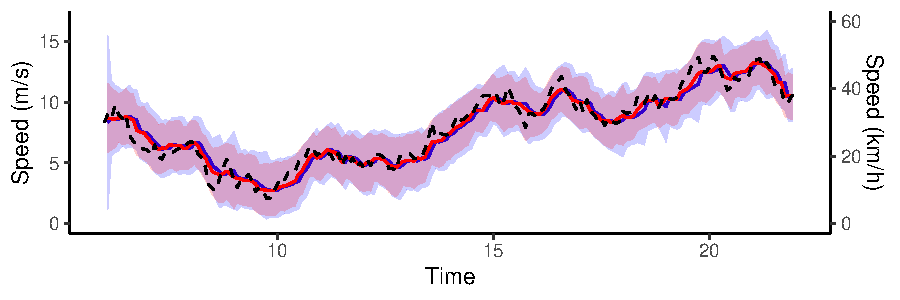
\includegraphics[width=.8\textwidth]{figure/nw_simdata_fit-1} }\\
\subfloat[Predictive distribution of average vehicle speed accounting for state uncertainty and between-vehicle uncertainty ($\NWvar^2$). Observations represented by black points.\label{fig:nw_simdata_fit2}]{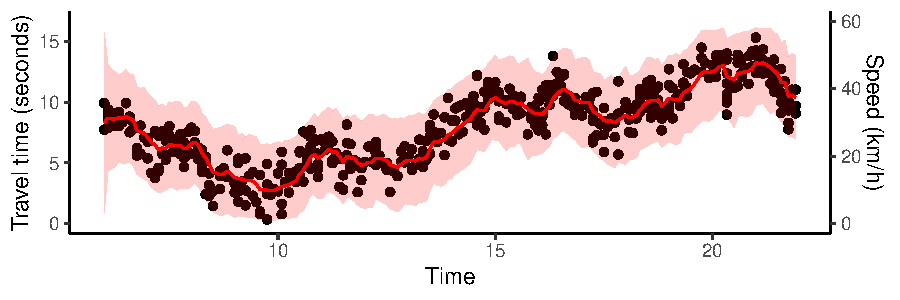
\includegraphics[width=.8\textwidth]{figure/nw_simdata_fit-2} }\\

}

\caption[Results of fitting the \kf{} to the simulated data]{Results of fitting the \kf{} to the simulated data.}\label{fig:nw_simdata_fit}
\end{figure}


\end{knitrout}

The \kf{} was fitted to the simulated data using the same values of $\NWnoise_\ell$ and $\NWvar_\ell$ used to generate the data, with the estimate of $\NWstate_{\ell,1:c}$ shown by the solid red line in \cref{fig:nw_simdata_fit1} along with the associated uncertainty as estimated by $\NWstatevar_{\ell,1:c}$ (shaded region). A dashed black line represents the simulated true mean. We see that the 95\% credible region contains the true values of $\NWstate_{\ell,1:c}$. \Cref{fig:nw_simdata_fit2} shows the posterior estimate of $\NWstate_{\ell,1:c}$ along with the posterior predictive distribution of $\NWobs_{\ellc}^m$; that is, using the 95\% region defined by the sum of $\NWstatevar_{\ell,1:c}$ and $\NWvar_\ell^2$, the latter of which is known for the simulation. 99.8\% of the observations lie within the 95\% predictive region. Given the network parameters $\NWnoise_\ell$ and $\NWvar_\ell$ are known, the underlying network state can be recovered using a \kf{}.


\subsection{Limitations of the implementations}
\label{sec:kf-limits}

The main limitation of using the information filter is the need to calculate the inverse of the covariance matrix. If we want to improve the model by including segment interactions, the dimensionality of $\NWstatevar$ would quickly become too large to compute $\NWstatevar^{-1}$ easily. Thus, the method presented here is only appropriate for independent segments. Fortunately, however, using the \kf{} instead would not be too difficult a task, since most of the time, only one vehicle will pass through a segment during an iteration. In cases where there is more than one, the estimates and their errors could be combined using a sample mean and variance, for example.


\section{Estimating network parameters}
\label{sec:nw_par_est}


To use the \kf{} in any meaningful way, we first need to estimate the system noise, $\NWnoise_\ell$, and the between-vehicle variance, $\NWvar_{\ell}^2$. To estimate values for these parameters, we fit the same model from \cref{sec:nw_model} to the historical data shown in \cref{fig:tt_figure} using \gls{mcmc} sampling methods as implemented by \prog{JAGS} \citep{JAGS}.


The first step in the modelling process fits the following hierarchical model:
\begin{equation}
\label{eq:nw_model_simple}
\begin{split}
\Vttobs_{\ellc}^m \cond \Vtt_{\ellc}^m &\sim \Normal{\Vtt_{\ellc}^m}{(\Vtterr_{\ellc}^m)^2}, \\
\Vtt_{\ellc}^m \cond \NWstate_{\ellc}, \NWvar_{\ell} &\sim \TNormal{\NWstate_{\ellc}}{\NWvar_{\ell}^2}{0}{\MaxSpeed_\ell}, \\
\NWstate_{\ell,0} &\sim \Uniform{0}{\MaxSpeed_\ell}, \\
\NWstate_{\ellc} \cond \NWstate_{\ell-1,c}, \NWnoise_\ell &\sim \TNormal{\NWstate_{\ell-1,c}}{(\NWtdiff_c \NWnoise_{\ell})^2}{0}{\MaxSpeed_\ell}, \\
\NWnoise_\ell &\sim \GammaD{0.01}{0.01}, \\
\NWvar_\ell &\sim \GammaD{0.01}{0.01}.
\end{split}
\end{equation}
The observation error, as in the previous section, is assumed to be constant for all observations, $\Vtterr_{\ellc}^m = 0.8$~\gls{mps} (which is about 10~km/h). The model implementation was performed from \Rstats{} using the \pkg{rjags} package \citep{rjags}. The model output was processed using the \pkg{tidybayes} package \citep{tidybayes} and graphed using \pkg{ggplot2} \citep{ggplot2}. The \pkg{coda} package was used to assess the model's convergence results \citep{coda}.


\subsection{Simulated data}
\label{nw_par_est_sim}

\begin{knitrout}\small
\definecolor{shadecolor}{rgb}{0.969, 0.969, 0.969}\color{fgcolor}\begin{figure}

{\centering 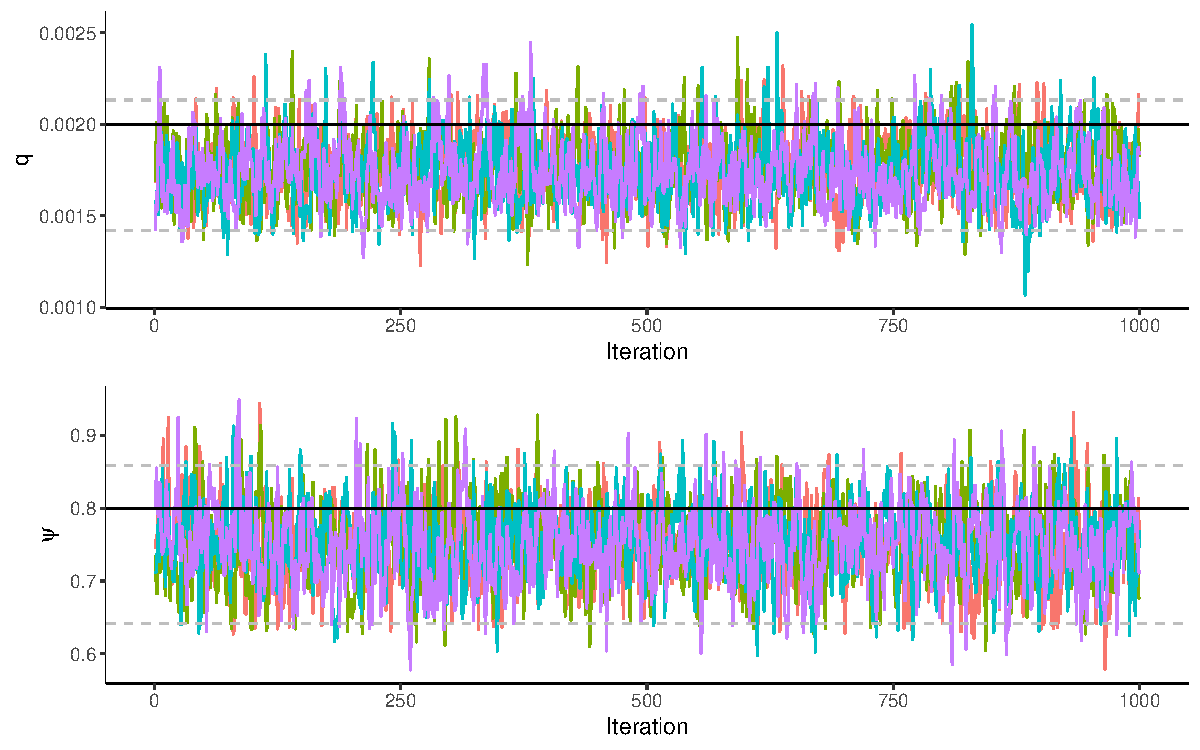
\includegraphics[width=0.8\textwidth]{figure/nw_model_sim_results-1} 

}

\caption[Traceplots of model parameters for the simulated data]{Traceplots of model parameters for the simulated data. Each of the four chains are coloured separately. Dashed grey lines show the 95\% posterior credible interval and the solid lines represent the true values or each parameter.}\label{fig:nw_model_sim_results}
\end{figure}


\end{knitrout}


To assess the model, we start by fitting it to the simulated data (\cref{fig:nw_sim_data}), for which we know the values of $\NWnoise_\ell$ and $\NWvar_\ell$. Trace plots of the model parameters shown in \cref{fig:nw_model_sim_results}, with the true values overlaid with a dashed line, show that the chains mixed well. \Cref{tab:nw_model_sim_smry} gives a summary of the simulation values and their posterior estimates, along with convergence statistics. The 95\% credible intervals for the two parameters contain the true values, so there is nothing to suggest the model is inadequate for modelling the simulated data and estimating the network parameters.


\begin{table}

\caption[MCMC results for the Bayesian model fitted to the simulated travel time data]{\label{tab:nw_model_sim_smry}MCMC results for the Bayesian model fitted to the simulated travel time data. The multivariate $\hat R$, including for all of the $\NWstate$ parameters, was 1.04, indicating that convergence had been achieved after 15,000 iterations.}
\centering
\begin{tabular}[b]{llllllr}
\toprule
Parameter & True Value & Mean & 2.5\% & 50\% & 97.5\% & $\hat R$\\
\midrule
$\NWnoise_\ell$ & 0.002 & 0.0017 & 0.0014 & 0.0017 & 0.0021 & 1.001\\
$\NWvar_\ell$ & 0.8 & 0.75 & 0.64 & 0.75 & 0.86 & 1.001\\
\bottomrule
\end{tabular}
\end{table}





\subsection{Real data}
\label{nw_par_est_real}



Having shown that the \prog{JAGS} model is a valid way of estimating the network parameters $\NWnoise_\ell$ and $\NWvar_\ell$, we model the real travel time data from \cref{fig:tt_figure}. Trace plots of the network parameters, as shown in \cref{fig:nw_model_n1_view}, show again that the chains mixed well, which is reaffirmed by the convergence results in \cref{tab:nw_model_fit_smry}. Not shown here are the summaries of the $\NWstate$'s (there are 187 of them); however, the Gelman diagnostic $\hat R$ was less than 1.03 for all of them, indicating they reached convergence.

\begin{knitrout}\small
\definecolor{shadecolor}{rgb}{0.969, 0.969, 0.969}\color{fgcolor}\begin{figure}

{\centering 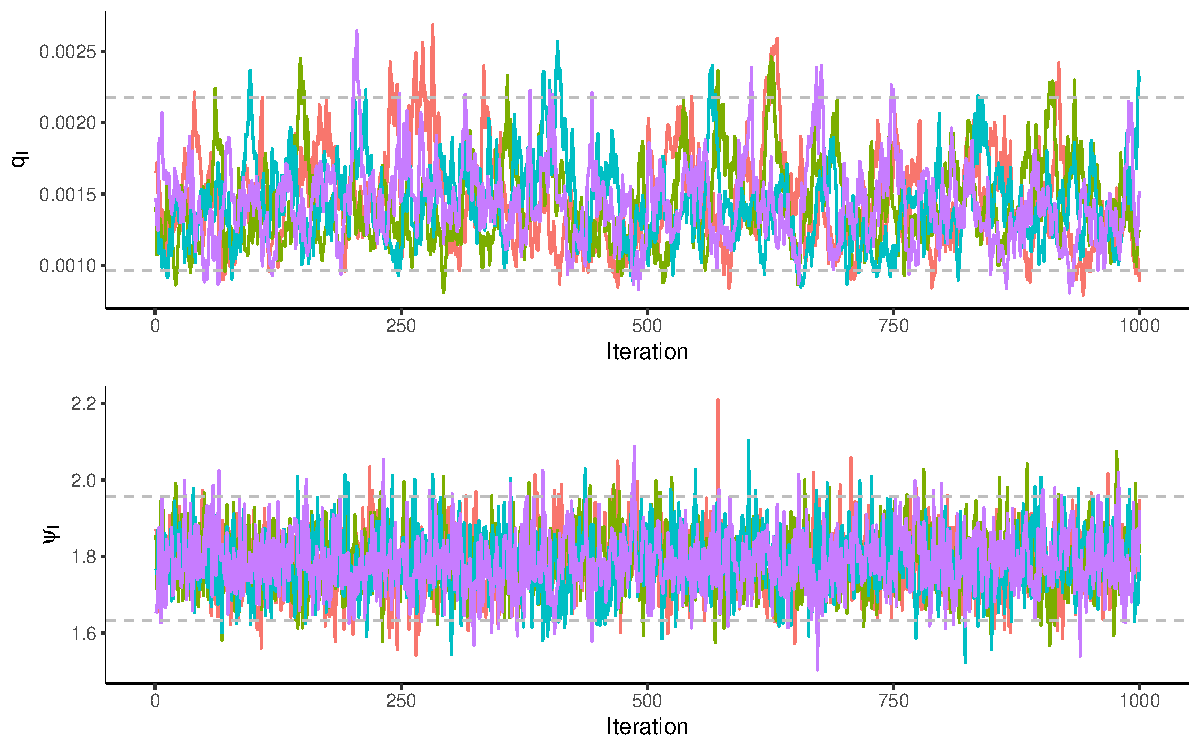
\includegraphics[width=0.8\linewidth]{figure/nw_model_n1_view-1} 

}

\caption[Traceplots of model parameters fitted to the segment data]{Traceplots of model parameters $\NWnoise$ and $\NWvar$ fitted to the segment data. Each of the four chains are coloured separately. The 95\% posterior credible region is denoted by dashed grey lines.}\label{fig:nw_model_n1_view}
\end{figure}


\end{knitrout}

\begin{table}

\caption[MCMC results for the Bayesian model fitted to the road segment travel time data]{\label{tab:nw_model_fit_smry}MCMC results for the Bayesian model fitted to the road segment travel time data. The multivariate $\hat R$, including for all of the $\NWstate$ parameters, was 1.08, indicating that convergence had been achieved after 15,000 iterations.}
\centering
\begin{tabular}[b]{lllllr}
\toprule
Parameter & Mean & 2.5\% & 50\% & 97.5\% & $\hat R$\\
\midrule
$\NWnoise_\ell$ & 0.0015 & 0.001 & 0.0015 & 0.0022 & 1.013\\
$\NWvar_\ell$ & 1.94 & 1.8 & 1.94 & 2.1 & 1.002\\
\bottomrule
\end{tabular}
\end{table}



To assess the adequacy of these parameters, we fit the \kf{} to the same data\footnote{In the next section we use two weeks of data, one for each of testing and training.} to see how well the mean and predictive distributions fit the data. The estimates of $\NWstate_{\ell,1:c}$, along with associated uncertainties, are shown in \cref{fig:nw_model_n1_kf1}, where we see that the mean approximately follows the center of the data. The predictive vehicle speed distribution, which accounts for both $\NWstatevar_{\ell,1:c}$ and between-vehicle uncertainty, $\NWvar_{\ell}$, is shown in \cref{fig:nw_model_n1_kf2}, and shows most of the points contained within the 95\% posterior predictive region.


\begin{knitrout}\small
\definecolor{shadecolor}{rgb}{0.969, 0.969, 0.969}\color{fgcolor}\begin{figure}

{\centering \subfloat[Estimated mean speed, showing state estimates along with the 95\% credible region.\label{fig:nw_model_n1_kf1}]{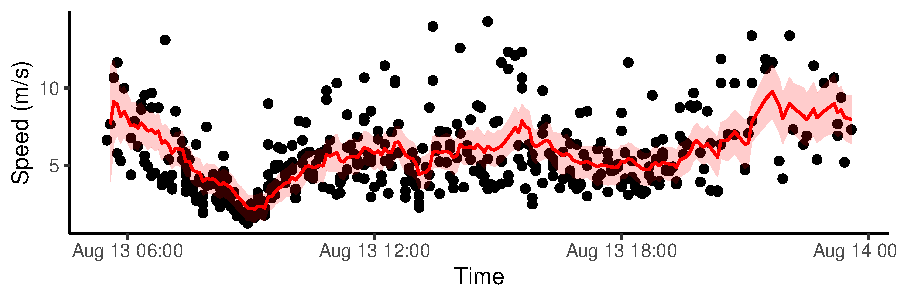
\includegraphics[width=.8\textwidth]{figure/nw_model_n1_kf-1} }\\
\subfloat[Predictive distribution of vehicle speeds, which includes between-vehicle variability.\label{fig:nw_model_n1_kf2}]{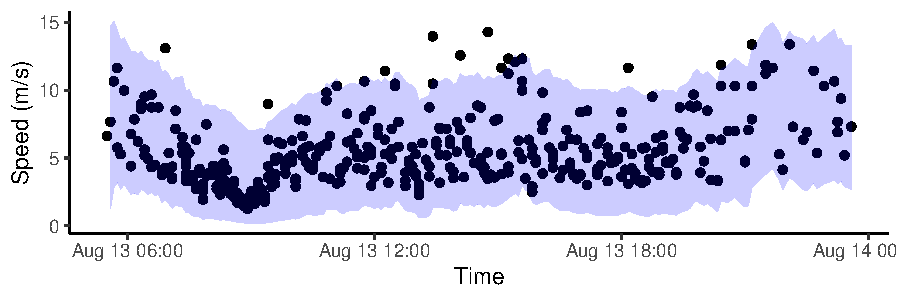
\includegraphics[width=.8\textwidth]{figure/nw_model_n1_kf-2} }\\

}

\caption[Results of fitting a \kf{} to the segment data with parameters estimated using the hierarchical model]{Results of fitting a \kf{} to the segment data with parameters estimated using the hierarchical model.}\label{fig:nw_model_n1_kf}
\end{figure}


\end{knitrout}



Finally, the timing comparison is displayed in \cref{tab:nw_model_n1_timecomp}. The hierarchical model fit using \prog{JAGS} took about 2200 times as long as the \kf{} implementation. So, even if we reduced the number of chains, the number of iterations, and tried to speed up the \prog{JAGS} model, the \kf{} would still be significantly faster.


\begin{table}

\caption[Comparison of the timings for the MCMC and \kf{} estimation methods]{\label{tab:nw_model_n1_timecomp}Comparison of the timings for the MCMC and \kf{} estimation methods. Times are reported in seconds.}
\centering
\begin{tabular}[b]{lrrr}
\toprule
  & User & System & Total\\
\midrule
JAGS & 124.828 & 0 & 124.847\\
Kalman filter & 0.052 & 0 & 0.056\\
\bottomrule
\end{tabular}
\end{table}




\subsection{Hierarchical model over multiple road segments}
\label{sec:nw_par_est_multiple}



To assess how effective our approach is for estimating $\NWvar_\ell$ and $\NWnoise_\ell$, we selected five other road segments around Auckland. However, instead of fitting the same model independently to each segment,  we use a hierarchical Bayesian model on the parameters, since it seems reasonable that, while they will not be the same for all segments, there will be an underlying population distribution. This allows us to obtain estimates of the parameter values without explicitly needing to model every road (of which there are 8,151).


The hierarchical model used to estimate the network parameters is:
\begin{equation}
\label{eq:tt_hist_hier}
\begin{split}
\Vttobs_{\ellc}^m \cond \Vtt_{\ellc}^m &\sim \Normal{\Vtt_{\ellc}^m}{\left(\Vtterr_{\ellc}^m\right)^2}, \\
\Vtt_{\ellc}^m \cond \NWstate_{\ellc}, \NWvar_{\ell} &\sim \TNormal{\NWstate_{\ellc}}{\NWvar_{\ell}^2}{0}{\MaxSpeed_\ell}, \\
\NWstate_{\ell0} &\sim \Normal{0}{10^2}, \\
\NWstate_{\ellc} \cond \NWstate_{\ellc-1}, \NWnoise_{\ell} &\sim \TNormal{\NWstate_{\ellc-1}}{(\NWtdiff_c \NWnoise_{\ell})^2}{0}{\MaxSpeed_\ell}, \\
q &\sim \GammaD{0.001}{0.001}, \\
\log\left(\NWvar_{\ell}\right) \cond \mu_\psi, \sigma_\psi &\sim \Normal{\mu_\psi}{\sigma_\psi^2}, \\
\mu_\psi &\sim \Normal{0}{10^2}, \\
\sigma_\psi &\sim \GammaD{0.001}{0.001}.
\end{split}
\end{equation}
We initially attempted to fit a hierarchical segment noise parameter $\NWnoise_{\ell}$ with hyper\-parameters, but the values were all approximately equal for all segments and convergence was very slow (100,000's of iterations). Instead, we opted for a single common system noise parameter across all segments. The speed data for six segments on two consecutive Tuesdays is shown in \cref{fig:nw_model_n2_segplots}, with the locations of the roads displayed in \cref{fig:nw_seg_maps}.

\begin{knitrout}\small
\definecolor{shadecolor}{rgb}{0.969, 0.969, 0.969}\color{fgcolor}\begin{figure}

{\centering 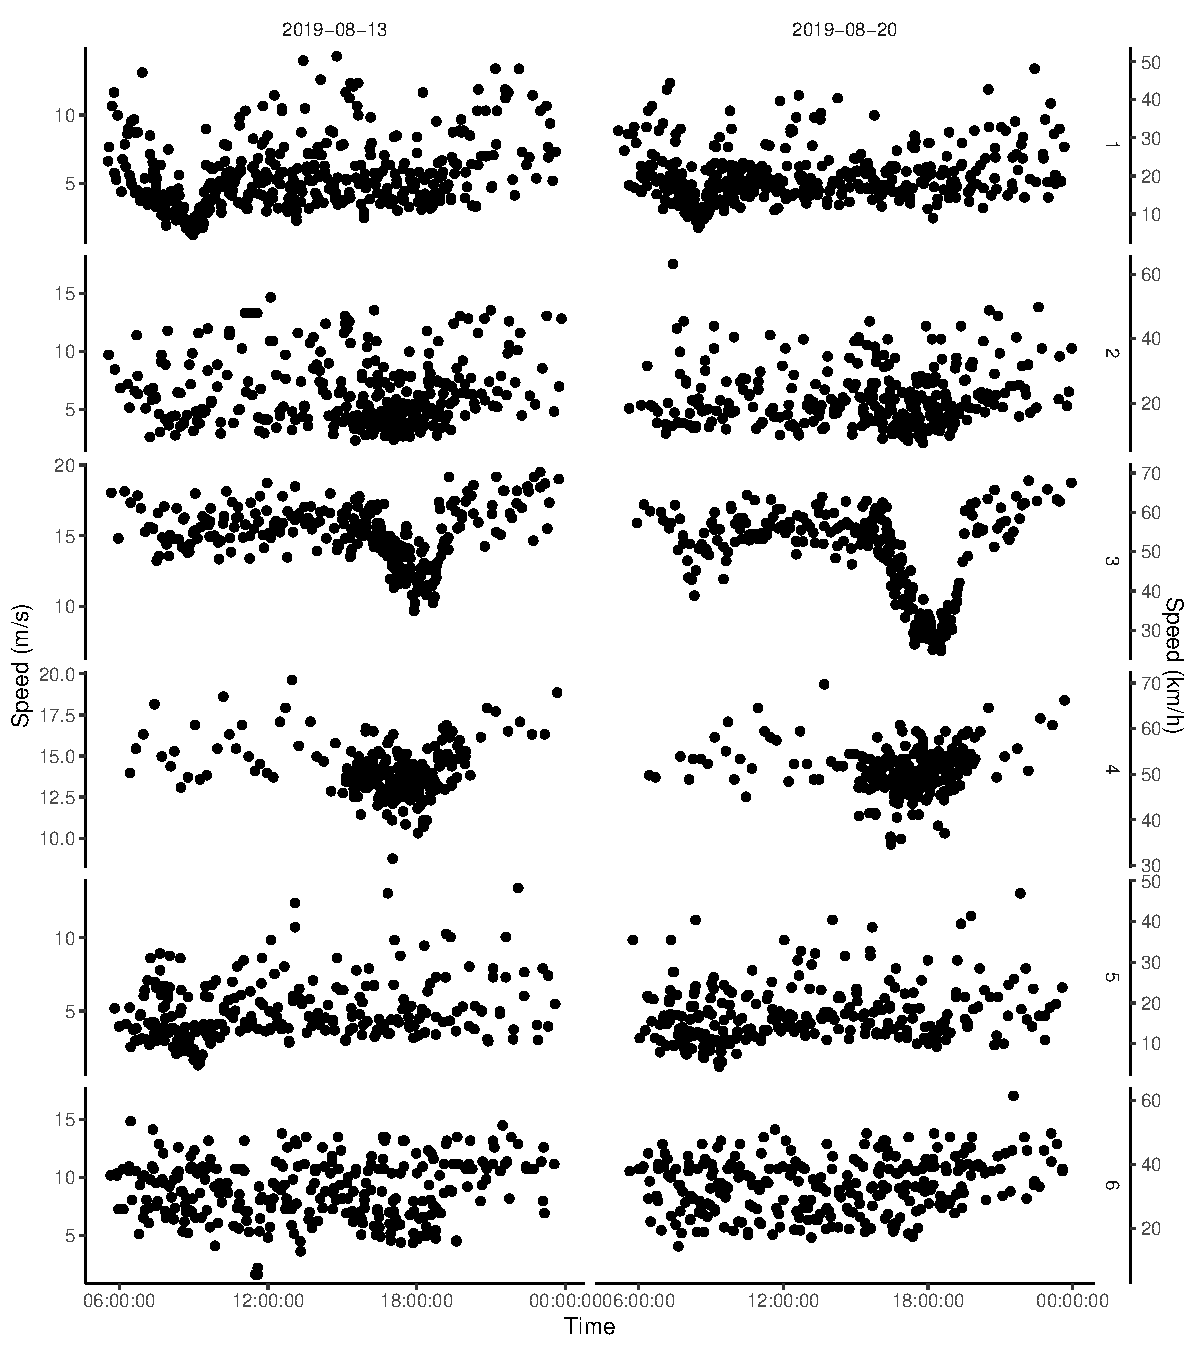
\includegraphics[width=\textwidth]{figure/nw_model_n2_segplots-1} 

}

\caption[Observed average bus speeds along six road segments on two consecutive Tuesdays]{Observed average bus speeds along six road segments on two consecutive Tuesdays.}\label{fig:nw_model_n2_segplots}
\end{figure}


\end{knitrout}

\begin{knitrout}\small
\definecolor{shadecolor}{rgb}{0.969, 0.969, 0.969}\color{fgcolor}\begin{figure}

{\centering 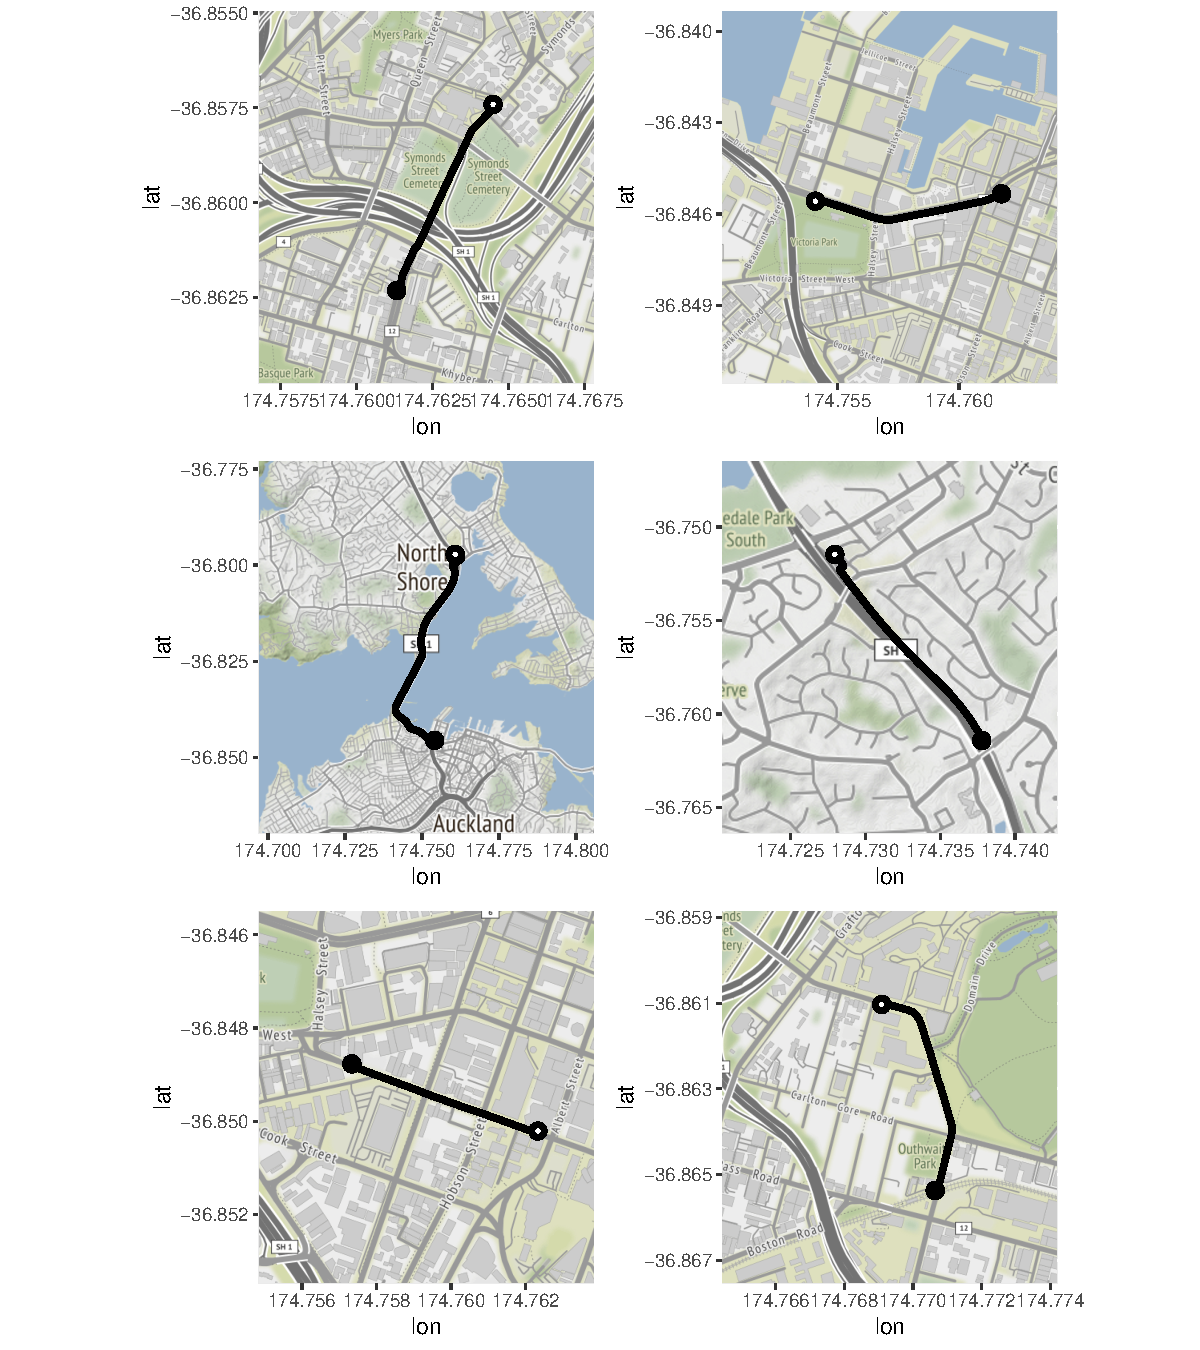
\includegraphics[width=\textwidth]{figure/nw_seg_maps-1} 

}

\caption[Segment locations, drawn using the \pkg{ggmap} package \citep{ggmap}]{Segment locations, drawn using the \pkg{ggmap} package \citep{ggmap}. Segments begin at the solid point and terminate at the open point.}\label{fig:nw_seg_maps}
\end{figure}


\end{knitrout}




\begin{knitrout}\small
\definecolor{shadecolor}{rgb}{0.969, 0.969, 0.969}\color{fgcolor}\begin{figure}

{\centering 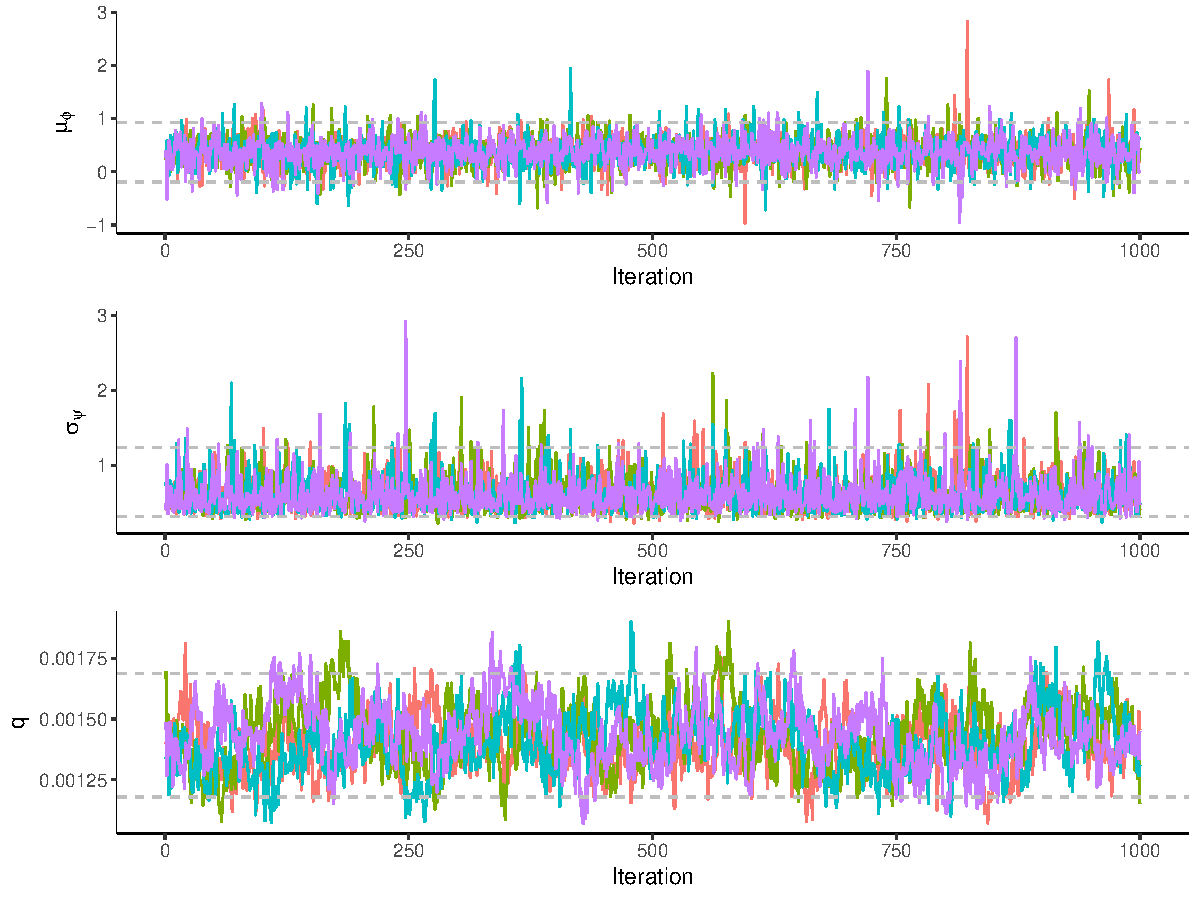
\includegraphics[width=\textwidth]{figure/nw_model_n2_diag-1} 

}

\caption[Traceplots of top-level network parameters estimated by the hierarhical model]{Traceplots of top-level network parameters estimated by the hierarhical model. The four chains are coloured individually, and 95\% credible interval indicated by dashed gray lines.}\label{fig:nw_model_n2_diag}
\end{figure}


\end{knitrout}


\begin{table}

\caption[MCMC results for the hierarchical Bayesian model fitted to six road segments to estimate the top-level variance parameters]{\label{tab:nw_model_n2_smry}MCMC results for the hierarchical Bayesian model fitted to six road segments to estimate the top-level variance parameters. The multivariate $\hat R$, including for all of the $\NWstate$ parameters, was 2.03.}
\centering
\begin{tabular}[b]{lllllr}
\toprule
Parameter & Mean & 2.5\% & 50\% & 97.5\% & $\hat R$\\
\midrule
$\mu_\psi$ & 0.383 & -0.191 & 0.389 & 0.926 & 1.00\\
$\sigma_\psi$ & 0.608 & 0.315 & 0.549 & 1.24 & 1.00\\
$q$ & 0.0014 & 0.0012 & 0.0014 & 0.0017 & 1.02\\
\bottomrule
\end{tabular}
\end{table}




The model was fit using \prog{JAGS} to the first day of data for the six segments, while the second was reserved for testing the validity of the estimated parameters. Each of the four chains was run with a 100,000~iteration burn-in phase, followed by 50,000 iterations with a thinning interval of 50. Trace plots of the top-level parameters are displayed in \cref{fig:nw_model_n2_diag}, which demonstrates good mixing of the chains. \Cref{tab:nw_model_n2_smry} shows the posterior mean and quantiles for these parameters, along with their Gelman convergence diagnostics.


Trace plots for the segment-specific variance parameters are shown in \cref{fig:nw_model_n2_diag_2}, and also demonstrate good mixing. The Gelman convergence diagnostic is again very close to unity, indicating that running the chain for longer would not decrease the posterior variance by much.



\begin{knitrout}\small
\definecolor{shadecolor}{rgb}{0.969, 0.969, 0.969}\color{fgcolor}\begin{figure}

{\centering 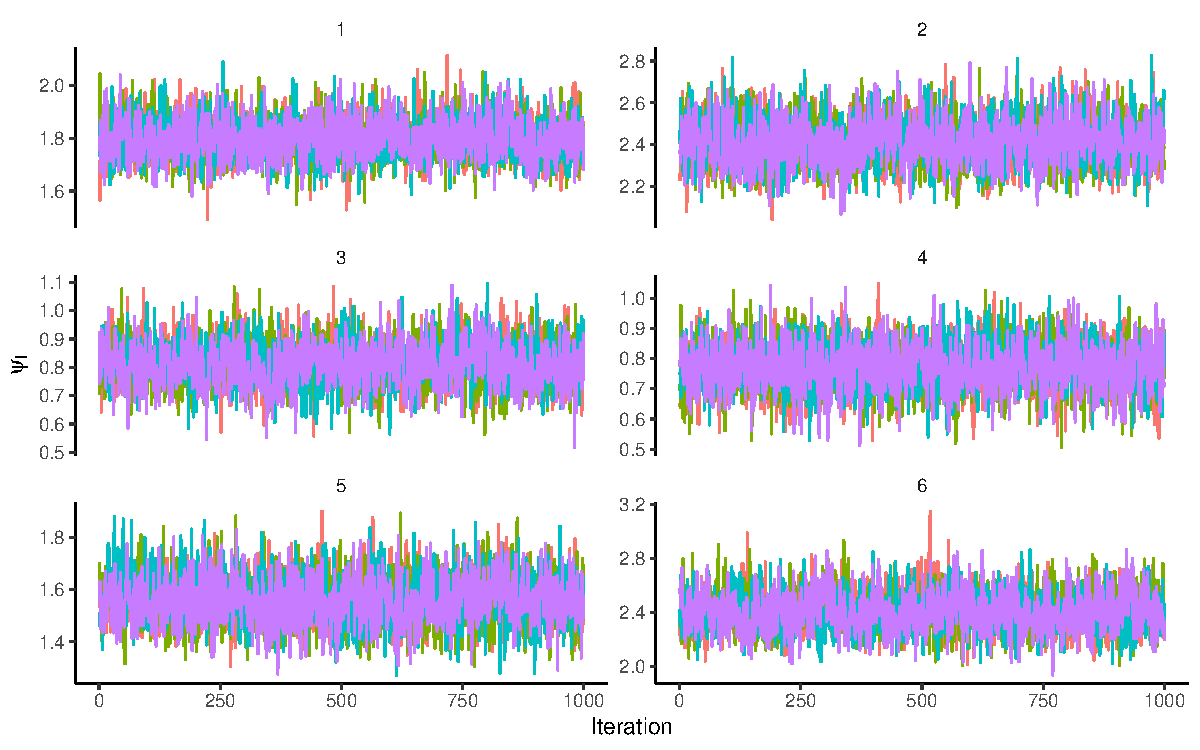
\includegraphics[width=\textwidth]{figure/nw_model_n2_diag_2-1} 

}

\caption[Traceplots of between-vehicle variance parameters, $\NWvar_\ell$, for each segment]{Traceplots of between-vehicle variance parameters, $\NWvar_\ell$, for each segment. The four chains are coloured individually.}\label{fig:nw_model_n2_diag_2}
\end{figure}


\end{knitrout}


The \kf{} was fit to each segment using the posterior mean of $\NWvar_\ell$ and the population parameters. \Cref{fig:nw_model_n2_kf} shows the original data superimposed with a posterior sample of $\NWstate$'s, along with the next week's data with results from the \kf{}, including the 95\% credible region for the mean road speed and the 95\% posterior predictive region for individual vehicles' average speeds.







\begin{knitrout}\small
\definecolor{shadecolor}{rgb}{0.969, 0.969, 0.969}\color{fgcolor}\begin{figure}
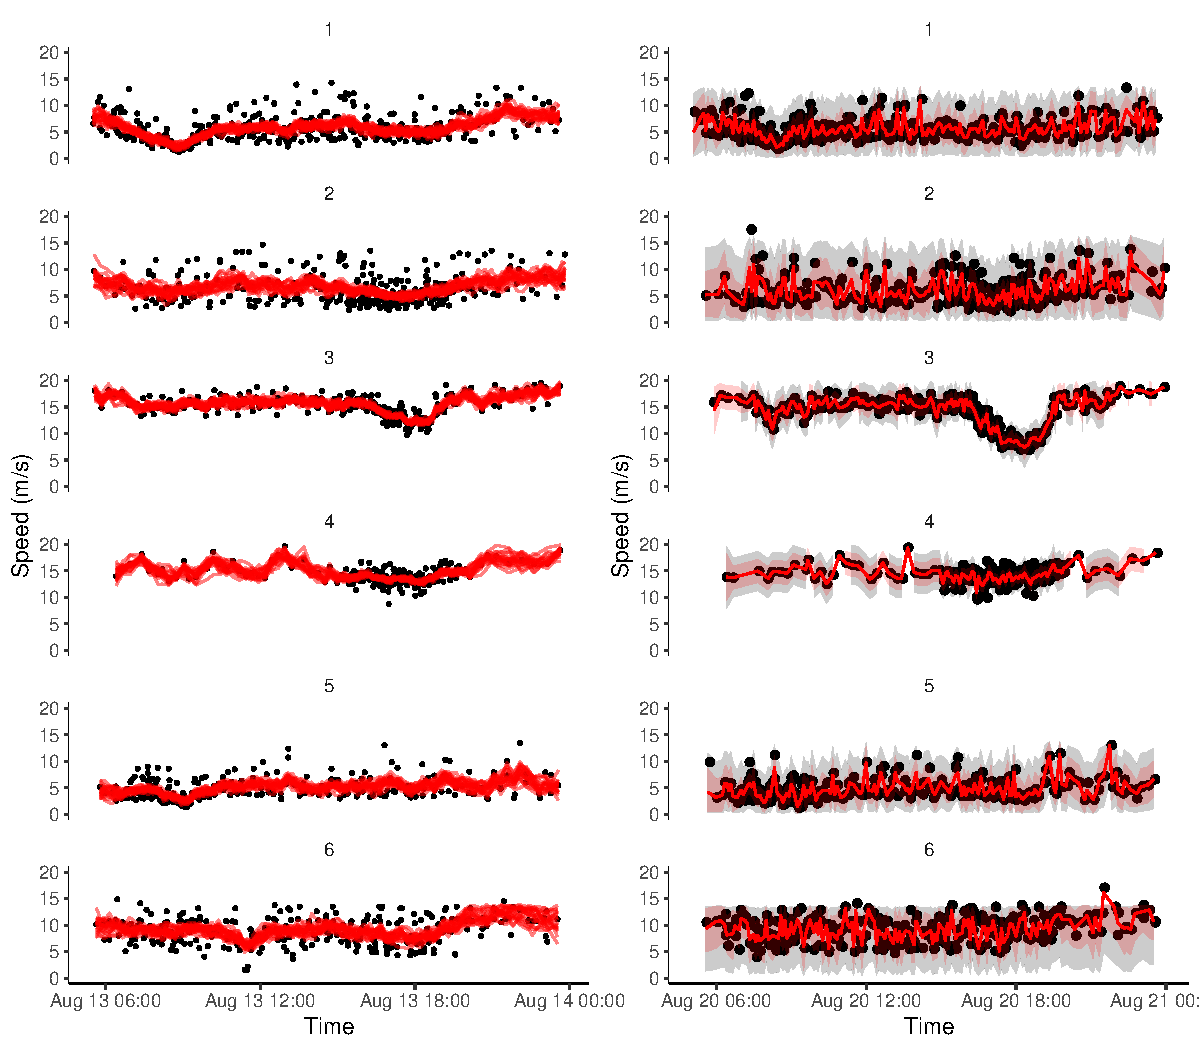
\includegraphics[width=\textwidth]{figure/nw_model_n2_kf-1} \caption[Results for the hierarchical approach to modelling road speed]{Results for the hierarchical approach to modelling road speed. Left: the training data with a sample of posterior fits for \prog{JAGS}. Right: the test data with the Kalman filter estimation results, showing the speed estimate (red line), its uncertainty (shaded in red), and the posterior predictive region for vehicle speeds (shaded in grey).}\label{fig:nw_model_n2_kf}
\end{figure}


\end{knitrout}

The results show that the $\NWstate$ values estimated with \prog{JAGS} nicely fit the data, including peak congestion, as do the \kf{} estimates. The posterior predictive region covers most of the observations for all the segments.

\section{Improving forecasts with history}
\label{sec:nw_hist_model}

The model presented in \cref{sec:nw_model,sec:nw_realtime,sec:nw_par_est} is adequate for estimating the \emph{real-time} state of the network, but is unuseful for forecasting vehicle speeds, particularly just before or after a peak period. In \cref{cha:prediction}, we explore the prediction of arrival times, which involves making short-term forecasts of speed. Using historical data is one way of improving speed forecasts, particularly around peak times.


In \cref{nw_par_est_real}, I showed that most roads have a ``peak effect'' in the morning or the evening, while some exhibit both. It seems reasonable therefore to have a model which allows a segment to have zero, one, or two peaks, each with varying magnitude (the size of the decrease in speed) and width (how long the peak period is). The temporal location of these peaks is likely to be related, but variable: some roads will experience peak traffic earlier than others, for example.

\begin{knitrout}\small
\definecolor{shadecolor}{rgb}{0.969, 0.969, 0.969}\color{fgcolor}\begin{figure}

{\centering 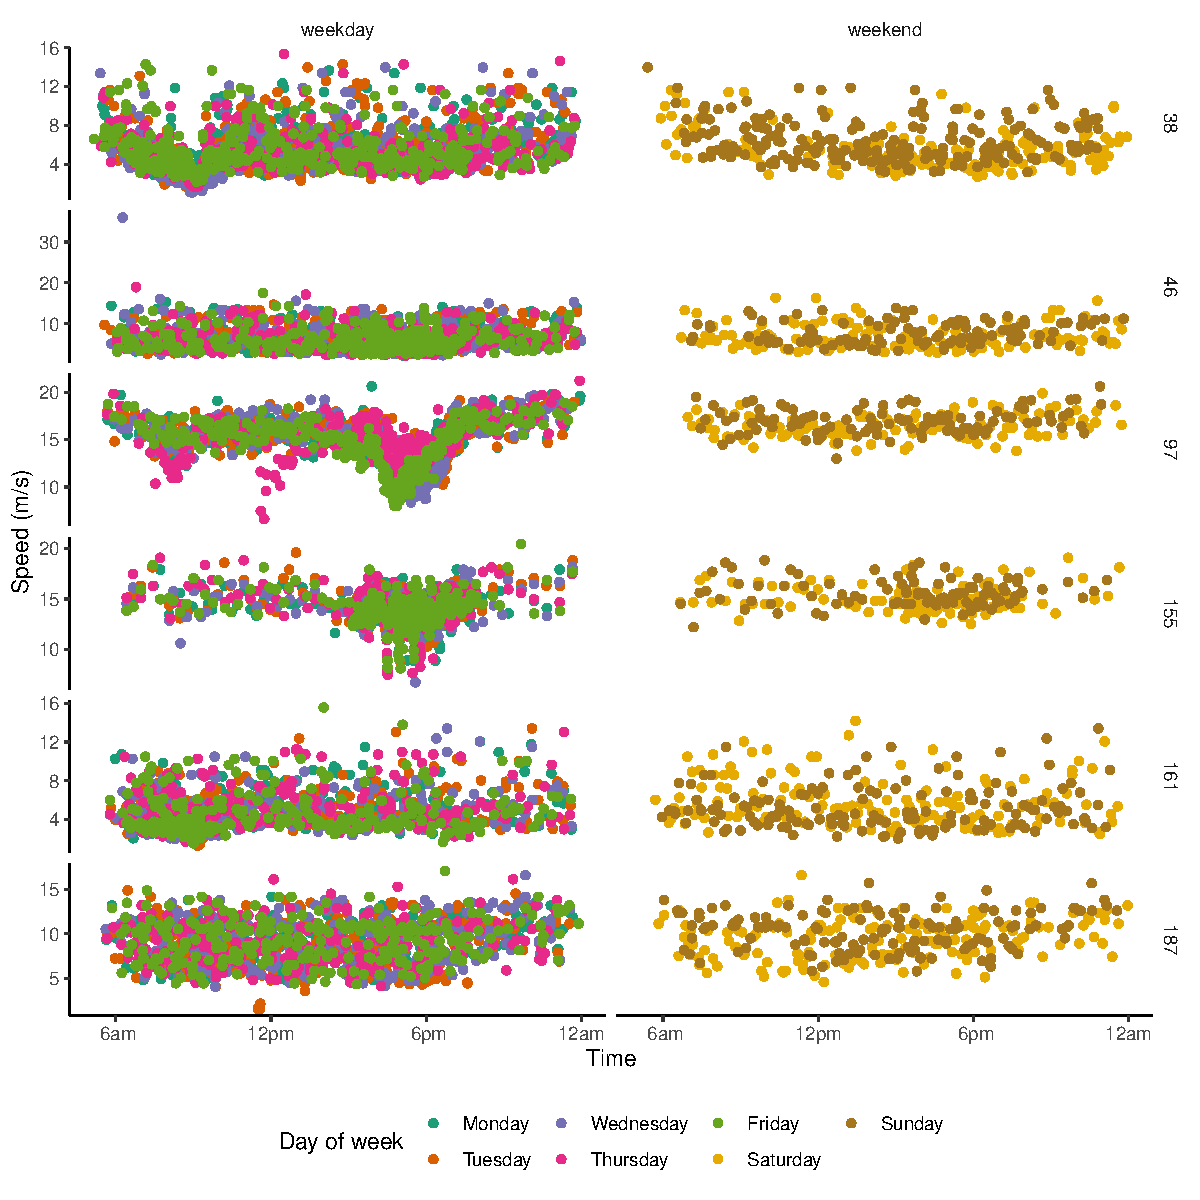
\includegraphics[width=\textwidth]{figure/tt_week0_load-1} 

}

\caption[Vehicle speeds along six road segments over one week]{Vehicle speeds along six road segments over one week, coloured by the day of the week.}\label{fig:tt_week0_load}
\end{figure}


\end{knitrout}

Early work fitting Bayesian models to these data were not promising, as it involved too much manual work tuning the parameters for each segment and checking the results. Since our goal is to obtain a generalised framework that runs with minimal manual effort, we sought an alternative.

From \cref{fig:tt_week0_load} it is clear that along each segment, there is a consistent pattern, with some variability between days as far as the temporal location and magnitude of the ``peak'' on weekdays; weekends are fairly consistent, although this is only two days' worth of data. Here I present a nearest-neighbour grid, which takes time and road state (traffic speed) as input, and outputs the mean (and uncertainty) of travel time in 10, 20, or 30~minutes from the current time. Similar ``speed maps'' have been used by the likes of \citet{Cathey_2003, Celan_2017, Chen_2014}. The first step is to aggregate observations into 5~minute intervals and take the mean traffic speed in each interval. Next, we bind lagged duplicates of these speeds (10, 20, 30~minutes, for example), such that each row includes current and future states. Any missing periods are interpolated from the mean of the adjacent states. The speed map for 30~minute predictions is shown in \cref{fig:tt_week0_grid}. The lighter areas represent higher speeds.







\begin{knitrout}\small
\definecolor{shadecolor}{rgb}{0.969, 0.969, 0.969}\color{fgcolor}\begin{figure}

{\centering \includegraphics[width=\linewidth]{figure/tt_week0_grid-1} 

}

\caption[Speed maps to predict segment speed in 30~minutes given the current state]{Speed maps to predict segment speed in 30~minutes given the current average speed (y-axis) and time (x-axis).}\label{fig:tt_week0_grid}
\end{figure}


\end{knitrout}

The next step is to evaluate the predictive power of this approach. We do this by taking the second week of data (shown in \cref{fig:tt_week1_load}) and use the fitted estimates to predict the state in 30~minutes, and then compare this to the actual state in 30~minutes. The \gls{rmse} (\cref{app:error-functions}) is used to compare the predicted and observed speeds.



\begin{knitrout}\small
\definecolor{shadecolor}{rgb}{0.969, 0.969, 0.969}\color{fgcolor}\begin{figure}

{\centering \includegraphics[width=\linewidth]{figure/tt_week1_load-1} 

}

\caption[Vehicle speeds along six roads over of two weeks.]{Vehicle speeds along six roads over the course of two weeks, showing only week days, for training (left) and testing (right).}\label{fig:tt_week1_load}
\end{figure}


\end{knitrout}

\begin{knitrout}\small
\definecolor{shadecolor}{rgb}{0.969, 0.969, 0.969}\color{fgcolor}\begin{figure}

{\centering \includegraphics[width=\linewidth]{figure/tt_week1_pred-1} 

}

\caption[Forecasts of average vehicle speeds in 30 minutes versus actual average speed in 30 minutes along segments]{Forecasts of average vehicle speeds in 30 minutes versus actual average speed in 30 minutes along segments. The line of equality (red) indicates a perfect prediction. The closer the best fit line (blue) is to the line of equality, the better the forecasts.}\label{fig:tt_week1_pred}
\end{figure}


\end{knitrout}


Forecasts 30~minutes into the future are shown in \cref{fig:tt_week1_pred} for both the grid-search method, as well as the na\"ive method of using the current average traffic speed as the predictor. The comparative \gls{rmse} values are displayed in \cref{tab:tt_pred_rmse}. However, these are not too different because there is a lot of inherent uncertainty, but demonstrate a slight increase in predictive performance when historical trends are used.


Most importantly, however, is the linear curve (shown in blue in \cref{fig:tt_week1_pred}) compared to the line of equality, in red. The interpretation is that the more accurate the predictions on average, the closer the blue trend line will be to the black line of equality. For our forecast model, we see that in 5 out of 6 segments the two lines are very close, compared to the na\"ive estimate in which case the predictions are often too high or too low.


Further work is needed to improve the forecasting abilities of our model. However, we have designed the framework in such a way that any such improvements can easily be integrated into both the network modelling stage, and the upcoming arrival time prediction stage (see \cref{sec:nw_implementation_forecast} for details).

\begin{table}

\caption{\label{tab:tt_pred_rmse}RMSE results comparing the predictive performance of the two models, in meters per second.}
\centering
\begin{tabular}[t]{lr}
\toprule
Method & RMSE\\
\midrule
Simple & 2.48\\
Forecast & 1.99\\
\bottomrule
\end{tabular}
\end{table}



\section{Particulars of the \rt{} implementation}
\label{sec:nw_implementation}

After stepping through the real-time model, estimation of its parameters, and improvement of forecasts using historical data, the last remaining piece of the network model is its real-time implementation within the \pkg{transitr} package. The first step is, of course, to load the historical data and model the real-time parameters using \prog{JAGS}. These are then inserted into the same database in which we store the \gls{gtfs} and network data.


The network is implemented as independent objects of class \class{Segment}, which are initialised when the program is first started with their model parameter values loaded---if available---from the database. The network state itself is implemented using the \pkg{Eigen} \Cpp{} library, allowing us to store the state vector and uncertainty matrix as an \verb+Eigen::Vector+ or \verb+Eigen::Matrix+, respectively. This library includes all the necessary vector and matrix operations, for example, multiplication. Even though the current state is one-dimensional, we may in future wish to extend this to include, say, the rate of change of speed, which could better model peak periods. This would involve a length-two state vector and $2\times2$ uncertainty matrix. By using \pkg{Eigen}, this change would require minimal code changes. The following sections discuss the initialisation, update, and prediction steps as implemented within \pkg{transitr}.


\subsection{Initialisation}
\label{sec:nw_implementation_init}

The initialisation phase of the network is quite important since in many cases it will be the only piece of information available for speed and arrival time predictions, at least until a vehicle traverses it and provides a real-time observation. Therefore, to initialise a \class{Segment}, we check if there is any historical data available for it: if there is, we set $\NWstate_{\ell,0}$ equal to the historical mean speed of all observations over time. To initialise the uncertainty, we use $\NWstatevar_{\ell 0} = \frac{30}{3.6^2}$~\gls{mps} (which is approximately 30~km/h).

Another part of initialisation is setting the constraint for the \emph{maximum speed}. Since we do not know the speed limit along most road segments, the best we can do is to use the maximum speed limit, 100~km/h, which is approximately 30~m/s. For segments with enough observations, we can use the maximum observed speed to estimate the posted speed limit along the road.



\subsection{State update}
\label{sec:nw_implementation_update}

The state update step is simple due to the segments being independent with one-dimensional states. First, \class{Segment}s are updated after processing the \class{Vehicle}s to collect any new observations (\cref{sec:vehicle_speeds}). Then we perform a parallel iteration over \class{Segment}s: if there are new observations, the update step (\cref{sec:nw_realtime}) is executed. The \pkg{Eigen} library makes this implementation straightforward. Once the state has been updated, the data vector is cleared and the \class{Segment}'s timestamp set to the current time.


\subsection{State forecasts}
\label{sec:nw_implementation_forecast}

While not part of the network state model, forecasting is an essential component of our real-time application. Each \class{Segment} has a \verb+forecast()+ method which returns the forecasted speed given the current timestamp\footnote{This is the time the \class{Segment} was updated, not the wall clock time.} and segment traffic speed. The forecasts are available in 10~minute intervals, so a forecast for 5~minutes uses the current travel time state, while a forecast for 25~minutes uses the 20-minute forecast, and so on, capped at 60~minutes. As for the uncertainty, this comes from the historical data too, but rather than forecasting, we use the historical variance of vehicle speeds at the desired time.

Currently, the forecast method uses the na\"ive constant-speed predictor. Since the arrival time prediction component (\cref{cha:prediction}) accesses forecasts through the \verb+Segment::forecast()+ method, an implementation of the historical-based forecasts\footnote{Or indeed any other desirable forecast method.} will automatically be integrated into the forecast model with no change needed to the prediction component.


\chapter{Predicting arrival time}
\label{cha:prediction}

So far, we have discussed the structure of transit data and its use in constructing a \emph{transit road network} (\cref{cha:data}) through which we model vehicles in real-time using a particle filter to estimate average vehicle speed along roads (\cref{cha:vehicle_model}). These speeds are, in turn, used to update a Kalman filter model of real-time road state (\cref{cha:network_model}). We now have everything needed to begin predicting the arrival time of buses at stops.

In this chapter, we introduce one final state which combines all of the information we have gained thus far. \emph{Trip state} provides a means of combining schedule information with real-time vehicle data to simplify the process of predicting stop arrival times, which also involves the network state and dwell-time information. The first step, therefore, is to estimate trip state (\cref{sec:trip_state}) based on the \gls{gtfs} schedule and estimated vehicle states from \cref{cha:vehicle_model}. Other frameworks have used a similar process, such as \citet{Cathey_2003}, who used a \emph{trip tracker} to prescribe real-time vehicle observations to trip states for use in the \emph{prediction} step.

The remainder of this chapter involves comparing a selection of four models---two using the real-time vehicle and network states, and two others for comparison (including the method currently in use in Auckland). \Cref{sec:prediction_arrival_time} presents the methods before we examine the results of arrival time prediction for a full day of observations for which we know the actual arrival time, allowing us to compare the performance of the methods (\cref{sec:prediction_model_comparison}). Lastly, we discuss the real-time implementation and performance results (\cref{sec:prediction_performance}) and assess the practicality of using a particle filter for arrival time prediction. This chapter focuses on the statistical properties of the prediction methods; practical issues are discussed in \cref{cha:etas}.


\section{Trip state}
\label{sec:trip_state}

At any one time, there are numerous scheduled trips within the transit network we want to obtain the \emph{state} of, which can then be updated with any real-time vehicle or network information, if available. Occasionally there is no vehicle associated with a given trip, so having a trip state makes it possible to combine schedule data with real-time network information to obtain \glspl{eta}. That is, it enables real-time arrival time prediction in the absence of real-time vehicle data.


At any time $t$, we obtain a list of scheduled trips such that the trip's start time $T_\text{start}$ is less than 30~minutes before $t$, and the trip's end time (arrival at last stop) is less than 60~minutes after $t$. The state of each trip within this window is represented by: $\Tript_k$, the time of the previous vehicle observation associated with it (if there is one); $\TripStop_k$, the current stop index; $\TripDep_k$, an indicator of whether the vehicle has departed from that stop; $\TripSeg_k$, the current segment index; and $\SegProg_k$, the progress (as a proportion) along the segment. These are stored in the trip state vector
\begin{equation}
\label{eq:trip_state}
\Tripr_k = \tvec{\Tript_k, \TripStop_k, \TripDep_k, \TripSeg_k, \SegProg_k}.
\end{equation}
The initial state is $\Tripr_0 = \tvec{T_\text{start},0,0,0,0}$. Trips use the same time subscript $k$ as vehicle locations since they are initialised based on the schedule, and then only updated when vehicle data is received.

Estimation of the various state components depends on the type of the most recent observation associated with the trip. The three possible scenarios are:
\begin{enumerate}
\item the last observation was a \emph{trip update} for stop $\TripStop$,
\item the last observation was a \emph{GPS position}, or
\item no data is available for the trip.
\end{enumerate}


\paragraph{Scenario 1:}
On arrival at stop $\TripStop$ at time $\Tript_k$, the trip's state is
\begin{equation}
\label{eq:trip_state_tu}
\Tripr_k =
\begin{cases}
\tvec{\Vtime_k, \TripStop, 0, \TripSeg(s), 0} & \text{if arrival}, \\
\tvec{\Vtime_k, \TripStop, 1, \TripSeg(s), 0} & \text{if departure},
\end{cases}
\end{equation}
where $\TripSeg(s)$ is the segment index of stop $\TripStop$.


\paragraph{Scenario 2:}
Here, the vehicle has completed travel along part of the segment, so the \emph{remaining distance} is needed. From the \pf{} in \cref{cha:vehicle_model}, the segment along which the vehicle is travelling at time $\Tript_k$ is identified as $\TripSeg_k$, and the most recently visited stop is $\TripStop_k$. The proportion of the segment travelled at time $t_k$, $\SegProg_k$, is easily calculated using the vehicle's current distance $\Vdist_k$ and the segment's start distance $\Tsegd_{\TripSeg_k}$ and length $\Tseglen_{\TripSeg_k}$:
\begin{equation}
\label{eq:trip_seg_completed_prop}
\SegProg_k = \frac{\Vdist_k - \Tsegd_{\TripSeg_k}}{\Tseglen_{\TripSeg_k}}.
\end{equation}


\paragraph{Scenario 3:}
There are three main reasons for there being no observations associated with a scheduled trip:
\begin{enumerate}
\item the trip has been cancelled, so no vehicle is servicing the trip, but the cancellation has not been entered into the real-time system;
\item the vehicle is late and has not yet started the trip; or
\item a vehicle is servicing the trip but its \gls{avl} system is either not working or is registered with the wrong trip.\footnote{This happens more often than one might first imagine.}
\end{enumerate}
There is no way to differentiate these three situations without physical investigation, so we always assume there is a bus travelling the route. However, if no bus has been observed, it is desirable to display a warning to passengers so that they are aware and can choose to catch an alternative bus instead.


It is common for passengers waiting at the first stops along a route to have no available \gls{rti} until the bus is a few minutes away. This is because the bus does not register with the server until it has begun the trip. Until this happens, the \gls{dms} displays the default scheduled time, which can be problematic if the bus is late to start the route. In extreme cases, once the scheduled time has passed the service disappears from the \gls{dms}, leaving passengers wondering whether the bus will eventually come, which is why it is necessary to display to commuters if no \gls{rti} is available for a trip.


Additionally, historical data of arrival times can be used in conjunction with the real-time network state to provide a prior estimate of arrival time, which is particularly useful for trips prone to starting late. In these situations, a single prediction is made when first initialising the trip based on historical information. Once the trip is observed (or cancelled) the prediction can be updated. The goal here is not to predict arrival times for unobserved vehicles accurately, but instead to smooth the arrival time estimates at the beginning of a trip's schedule for those situations where the vehicle does finally start its route.

\section{Arrival time prediction methods}
\label{sec:prediction_arrival_time}




\begin{knitrout}\small
\definecolor{shadecolor}{rgb}{0.969, 0.969, 0.969}\color{fgcolor}\begin{figure}

{\centering \includegraphics[width=\linewidth]{figure/layover_observance-1} 

}

\caption[Vehicle delays at layover stops truncated to 10~minutes early and 20~minutes late]{Vehicle delays at layover stops truncated to 10~minutes early and 20~minutes late. Negative values indicate non-adherance by drivers, which makes up 40\% of cases.}\label{fig:layover_observance}
\end{figure}


\end{knitrout}

The estimated trip state (and any associated vehicle) and the road network can now be combined to forecast how long it will take for the vehicle to reach all remaining stops along the route. Dwell times can also affect arrival time uncertainty. Some trips have the added complexity of layovers at specific stops---these are common at major points of interest, such as at a mall, or stations where many routes connect so passengers can transfer between services (see \cref{sec:gtfs}). In theory, drivers wait at these stops until the scheduled departure time before continuing the trip; however, in 40\% of cases over two weeks, the driver left before the scheduled departure time, as is demonstrated in \cref{fig:layover_observance}, and 31\% departed more than one minute early.


There are various ways to forecast arrival times, each with associated drawbacks and advantages. This section presents four arrival time prediction methods:
\begin{itemize}
\item \Fpf{} uses the particle filter estimate of vehicle state and the network state to obtain arrival time distributions;
\item \Fnorm{} uses a normal approximation of the vehicle's state, along with the network state and dwell-time distributions;
\item \Fhist{} uses only historical delay data; and
\item \Fsched{} uses the schedule and current real-time delay, as is currently used by \AT{}.
\end{itemize}
The first two use the network state, which is simplified for each route by including only the segments (in order) used by route $r$ with mean and variance
\begin{equation}
\label{eq:route_nw_state}
\RouteNWstate^r =
\begin{bmatrix}
\RouteNWstateseg^r_1 \\
\RouteNWstateseg^r_2 \\
\vdots \\
\RouteNWstateseg^r_L
\end{bmatrix}\quad\text{and}\quad
\RouteNWstatevar^r =
\begin{bmatrix}
\RouteNWstatevarseg^r_{1} & \RouteNWstatecor^r_{1,2} & \cdots &\RouteNWstatecor^r_{1,L} \\
\RouteNWstatecor^r_{2,1} & \RouteNWstatevarseg^r_{2} & \ddots &\RouteNWstatecor^r_{2,L} \\
\vdots & \ddots & \ddots & \vdots \\
\RouteNWstatecor^r_{L,1} & \RouteNWstatecor^r_{L,2} & \cdots & \RouteNWstatevarseg^r_L
\end{bmatrix},
\end{equation}
respectively, where $\RouteNWstateseg^r_{i}$ is the average vehicle speed along the $i$th segment of route $r$, $\RouteNWstatevarseg^r_{i}$ is the variance for the segment, and $\RouteNWstatecor^r_{i,j}$ is the covariance between segments $i$ and $j$. Note that the current implementation does not include segment covariances, but the above setup demonstrates that the model can include them, if available. To simplify notation, I have dropped the $r$ superscript for the remainder of this chapter since only one route is dealt with at any one time.

For bus stop dwell times, we collected two weeks' of data (as was used in \cref{sec:nw_par_est}) and calculated the mean and variance of dwell time for all stops along each trip. It is possible to determine if a bus \emph{did} stop (there is both an arrival and a departure time), but not that a bus \emph{did not} stop. For example, if the bus reports only an arrival time, it is unclear whether this is because the bus truly did not stop, or if it is a deficiency with the data. The bus may not have reported both observations, or, more likely, the polling interval (30 seconds) did not see both of them (Auckland Transport's real-time feed only includes the most recent observation). Therefore, stopping probabilities cannot be estimated from the data, so the same value of $\Prstop_j=0.5$ is used as in \cref{cha:vehicle_model}.


\subsection{Particle filter (\Fpf{})}
\label{sec:prediction_arrival_time_pf}

Each active trip is associated with a single vehicle, itself associated with a set of  $\Np$~particles approximating the vehicle's state. Perhaps the most straightforward method---at least conceptually---of predicting arrival times is to let each particle progress to the end of the route and record its arrival times. Computationally, this is easy to implement but very intensive, significantly increasing iteration time for the application. However, as we no longer need to worry about updating (via importance resampling), we can use a smaller subset of particles, $\Np^\star \leq \Np$, which can be adjusted depending on how many stops there are along the remainder of the route.

\begin{itemize}
\item better argument for using smaller $N$
\item rewrite paragraph below more succinctly (perhaps as a list)
\item for the dwell time stuff, refer back to Ch 3
\end{itemize}


To implement the particle filter forecast method, which we denote \Fpf{}, we take a (weighted) subsample of $\Np^\star$ particles at time $\Vtime_k$, $\tilde\Vstate_k$ (the time of the most recent vehicle observation). For each particle, we calculate the arrival time at each upcoming stop. First, if the particle is at a stop,  the ``remaining travel time'' for the current segment is needed, which we calculate by taking the particle's current speed, adding some noise, and extrapolating to the end of the segment. Having completed the current (partial) segment $j$, the particle's travel time to stop $j$, $\Linkt\vi_j$, is used to estimate the arrival time,
\begin{equation}
\label{eq:particle_arrival_time}
\Tarr\vi_j = \Vtime + \Linkt\vi_j.
\end{equation}
Next, we iteratively add dwell time and travel time for stops and road segments, respectively, until the particle reaches the end of the route; alternatively, we could stop after some number of stops, as we discuss in \cref{sec:prediction_performance}. The dwell time is assumed Gaussian with mean and variance estimated from historical data, $\mu_{\dwell_j}$ and $\sigma_{\dwell_j}$, respectively:
\begin{equation}
\label{eq:prediction_dwell_time}
\begin{split}
\Istop\vi_j &\sim \Bern{\Prstop_j} \\
\pserve\vi_j &\sim \TNormal{\mu_{\dwell_j}}{\sigma_{\dwell_j}}{0}{\infty} \\
\pdwell\vi_j &= \Istop\vi_j \pserve\vi_j
\end{split}
\end{equation}


\begin{itemize}
\item better clarification of terms here
\end{itemize}

When estimating travel time, the particle's speed along each segment is drawn from the network state,
\begin{equation}
\label{sec:particle_travel_time_pred}
\Linkt\vi_j \sim
\Normal{\hat\RouteNWstateseg_j}{
  (P_j + \Delta_j\NWnoise)^2)\wedge\mu_{P_j}
},
\end{equation}
which allows uncertainty to increase for more temporally distant forecasts, with a maximum set by the historical (prior) uncertainty.


Having obtained arrival times for all $\Np^\star$ particles, the predictive distribution for stop $j$---as in \cref{cha:vehicle_model}---is simply
\begin{equation}
\label{eq:particle_predictive_dist}
p(\Tarr_j | \Tripr_k, \RouteNWstate_\Tripr) \approx
\sum_{i=1}^{\Np^\star} \Pwt \dirac_{\Tarr_j\vi}\left(\Tarr_j\right)
= \frac{1}{\Np^\star}\sum_{i=1}^{\Np^\star} \dirac_{\Tarr_j\vi}\left(\Tarr_j\right)
\end{equation}
since all weights are equal. From the particle approximation of the distribution of arrival times we obtain point estimates or quantiles---for example, the mean, median, or a 90\% credible region. As discussed in \cref{app:particle-summaries}, computing quantiles (including the median) is a computationally demanding task for large numbers of particles due to the necessity to sort the particles in order from earliest to latest arrival times---at each stop.

\subsection[Normal approximation]{Normal approximation (\Fnorm{})}
\label{sec:prediction_arrival_time_normal}

Due to the computational demand of the particle filter, significant speed improvements can be obtained by using a normal approximation instead. The network state is a multivariate normal random variable, so the issue lies with stop dwell times having a point mass at zero, resulting in a mixture predictive distribution. For each stop the vehicle passes, there are twice as many components, so after $m$ stops, there are $2^m$ components. However, these regularly converge after a few stops, as shown in \cref{fig:normal_approx}.

\begin{knitrout}\small
\definecolor{shadecolor}{rgb}{0.969, 0.969, 0.969}\color{fgcolor}\begin{figure}

{\centering \includegraphics[width=\textwidth]{figure/normal_approx-1} 

}

\caption[Normal approximation for a series of stops ahead]{Normal approximation for a series of stops ahead. The true distribution is shown by the histogram with the underlying components (dashed curves). The vertical lines represent the quantiles computed using the sampled data, the normal mixture (using the optimisation formula), or a single normal approximation.}\label{fig:normal_approx}
\end{figure}


\end{knitrout}

A mixture of normal distributions can approximate the arrival time distribition \citep{Wang_2012} by expressing the mean and uncertainty as vectors $\tilde\mu$ and $\tilde\sigma^2$, respectively, along with a third vector $\tilde\pi$ denoting the $\tilde N$ mixture weights\footnote{We are using the tilde over parameters, e.g., $\tilde x$, to help distinguish them from others used throughout the thesis}, such that
\begin{equation}
\label{eq:ch5:mixture_weight_spec}
\tilde\pi_i > 0, i = 1, \ldots, \tilde N
\text{ and } \sum_{i=1}^{\tilde N} \tilde\pi_i = 1.
\end{equation}
The arrival time at stop $j + n$ is then given by
\begin{equation}
\label{eq:arrival_time_normal_approx}
\Tarr_{j+n} | \tilde\mu, \tilde\sigma^2, \tilde\pi, \RouteNWstate =
\sum_{\ell=j}^{j+n-1} \RouteNWstateseg_\ell +
\sum_{i=1}^{\tilde N} \tilde\pi_i z_i,\quad
z_i \sim \Normal{\tilde\mu_i}{\tilde\sigma^2_i}.
\end{equation}


Each component $i$ has an indicator $I_{im} = \{0,1\}$ of whether or not it stopped at stop $m$, so the total dwell time has mean and variance
\begin{equation}
\label{eq:mixture_dwell_times}
\tilde\mu_i = \sum_{m=j}^{j+n} I_{im} \dwell_m\quad\text{and}\quad
\tilde\sigma_i^2 = \sum_{m=j}^{j+n} I_{im} \dwellvar_m,
\end{equation}
respectively, assuming dwell times at individual stops are independent of each other.

Mixture weights are obtained through the stopping probability at each stop, $\pi_j$:
\begin{equation}
\label{eq:ch5:mixture_weights}
\tilde\pi_i = \prod_{m=j}^{j+n} \tilde p_{im}
\end{equation}
where
\begin{equation}
\label{eq:ch5:mixture_weights2}
\tilde p_{im} =
\begin{cases}
\pi_m & \text{if } I_{im} = 1 \\
1 - \pi_m & \text{otherwise.}
\end{cases}
\end{equation}


The mixture approximation works well for a few stops ahead, but after some time the mixture weights become small and the components combine, as shown in \cref{fig:normal_approx}. To prevent $\tilde N$ from becoming too large, the full distribution is simplified into a single component with mean and variance
\begin{equation}
\label{eq:mixture_mean}
\begin{split}
\E{\Tarr_m | \tilde\pi, \tilde\mu, \tilde\sigma^2, \RouteNWstate} &=
\E{\sum_{\ell=j}^{j+n-1} \RouteNWstateseg_\ell +
  \sum_{i=1}^{\tilde N} \tilde\pi_i z_i} \\
&= \sum_{\ell=j}^{j+n-1} \E{\RouteNWstateseg_\ell} +
  \sum_{i=1}^{\tilde N} \tilde\pi_i \E{z_i} \\
&= \sum_{\ell=j}^{j+n-1} \hat\RouteNWstateseg_\ell +
  \sum_{i=1}^{\tilde N} \tilde\pi_i \tilde\mu_i
\end{split}
\end{equation}
and
\begin{equation}
\label{eq:mixture_variance}
\begin{split}
\Var{\Tarr_m | \tilde\pi, \tilde\mu, \tilde\sigma^2, \RouteNWstate} &=
\Var{\sum_{\ell=j}^{j+n-1} \RouteNWstateseg_\ell +
  \sum_{i=1}^{\tilde N} \tilde\pi_i z_i} \\
&= \sum_{\ell=j}^{j+n-1} \Var{\RouteNWstateseg_\ell} +
  \sum_{i=1}^{\tilde N} \tilde\pi_i^2 \Var{z_i} \\
&= \sum_{\ell=j}^{j+n-1} \hat\RouteNWstatevarseg_\ell +
  \sum_{i=1}^{\tilde N} \tilde\pi_i \tilde\sigma_i^2
\end{split}
\end{equation}
respectively, assuming segment travel time and dwell time are independent---assuming otherwise makes this model impossible to work with; indeed, this model versus the particle filter (which makes no such assumption) is effectively testing the viability of this assumption.


An optimisation is used to obtain quantiles $q_\alpha$ such that
\begin{equation}
\label{eq:mixture_quadratic}
\left[
  p\left(\alpha \leq \Tarr_m | \tilde\pi, \tilde\mu, \tilde\sigma^2, \RouteNWstate\right) - q_\alpha
\right]^2 = 0.
\end{equation}
This is straightforward using Brent's Algorithm \citep{Brent_1971}, implemented in the Boost \textsf{C++} library.

When the 2.5\%, 50\%, and 97.5\% quantiles for the single approximation are within 30~seconds of the same quantiles computed for the mixture distribution, the mixture is replaced with one single component with mean and variance defined in \cref{eq:mixture_mean,eq:mixture_variance}. In some situations, the mixture may not converge into a single distribution quick enough, so to prevent the number of components $\tilde N$ from exceeding $2^8=256$, all components with weights less than a predefined threshold (we used $\frac{1}{2}\max_i(\pi_i)$) are combined into a single component.


%%%%%%%%%%%%%%%%%%%%%%%%%%%%%%%%%%%%%%%%%%%%%%%%%%%%%%%%% Historical data
\subsection{Historical arrival delays (\Fhist{})}
\label{eq:prediction_arrival_historical}

Another way to make predictions is to use historical data instead of real-time. We collected two weeks of data and recorded arrival time delays by stop and route to obtain a distribution which can then be used to make predictions. The arrival time at stop $j$ along route $r$ has an average delay of $\bar d_{rj}$ seconds with variance $D_{rj}^2$, so the predicted arrival time at stop $j$ on route $r$ with scheduled arrival time $S_{rj}$ is
\begin{equation}
\label{eq:arrival_pred_historical}
\hat\Tarr_{j} \sim \Normal{S_{rj} + \bar d_{rj}}{D_{rj}^2}.
\end{equation}


%%%%%%%%%%%%%%%%%%%%%%%%%%%%%%%%%%%%%%%%%%%%%%%%%%%%%%%%% Schedule + delay
\subsection{Schedule delays (\Fsched{})}
\label{eq:prediction_arrival_sched_delay}

The currently deployed prediction method uses the scheduled arrival time at stop $j$ along route $r$, $S_{rj}$, along with the arrival or departure time at the most recently visited stop, $T_{rm}$, giving a current delay, in seconds, of
\begin{equation}
\label{eq:sched_cur_delay}
d_{r} = T_{rm} - S_{rm}.
\end{equation}
The arrival time is then predicted as
\begin{equation}
\label{eq:sched_pred_arr}
\hat\Tarr_{rj} = S_{rj} + d_r.
\end{equation}
Note, however, that if a trip has not yet been observed, the default delay is $d_r = 0$, regardless of whether or not there is a vehicle servicing it, the vehicle is running late, or the trip has been cancelled altogether.

\section{Assessing predictive performance}
\label{sec:prediction_model_comparison}


To compare the four prediction methods, we implemented the first two in the \textsf{transitr} application and, using a single day of data, run the program, storing all arrival time estimates, the uncertainty, as well as the 5\% and 90\% quantiles\footnote{Initially we used a symmetric 95\% prediction interval, but this was often highly skewed by a few very late particles.}. The actual (reported) arrival times are then used to compare the accuracy of each method. For the historical data, we compare the mean with the actual arrival time. For the schedule-delay method, the arrival time for all upcoming stops was predicted after each new observation, and the prediction error computed.

\begin{itemize}
\item yes, rewrite the above para to make more sense please.
\item and, the below might need some more words about MAE/MAPE \ldots
\end{itemize}

We used \gls{rmse}, \gls{mae}, and \gls{mape} as comparison criteria (see \cref{app:error-functions}).
\Gls{rmse} is the mean squared difference (in seconds) between the predicted and actual arrival times. Of course, since predictions change over time, we also compute \gls{rmse} by \emph{time until (actual) arrival}, allowing us to compare the models at different time points, as well as by stop sequence and time of day.


Another criteria we are interested in is the \gls{picp}, which is only available for the three methods for which we can construct an 85\% \gls{ppi}: for the particle filter, this is achieved by sorting the particles in order of arrival time, and then taking the $\lfloor q_\text{lower} N^\star\rfloor^{\text{th}}$ particle as the lower bound, and the $\lceil q_{\text{upper}} N^\star\rceil^{\text{th}}$ particle as the upper bound (more details in \cref{app:particle_summaries}). For the 85\% interval, we used $q_\text{lower} = 0.05$ and $q_\text{upper} = 0.9$. For the normal approximation and historical arrival methods, the inverse \gls{cdf} provides the required quantiles. The results are displayed in \cref{tab:model_results_rmse} and \cref{fig:model_results_rmse_time,fig:model_results_rmse_stopn,fig:model_results_rmse_timeofday} (described in \cref{sec:prediction_model_comp_stats}).


\begin{itemize}
\item predictive power, or `reliability'?
\end{itemize}

Additionally, we also want to compare the predictive power of the various forecast methods, namely \emph{the probability of arriving before the bus}, and hence not missing it, as well as the expected waiting time given a passenger arrives at the stop by a certain time. In table \cref{tab:model_results_pr_miss} and \cref{fig:model_results_pr_gtfs,fig:model_results_pr_time,fig:model_results_pr_stop,fig:model_results_pr_timeofday}, we use the point estimate (mean or median, depending on the forecast method), as well as the 5\% quantile, and for each calculate the probability that the bus arrives after the specified time. We also calculate the expected waiting time for a passenger arriving at a certain time \emph{and the bus arrives after the specified time} (i.e., the passenger catches the bus). \Cref{sec:prediction_model_comp_probs} discusses these results.






\begin{knitrout}\small
\definecolor{shadecolor}{rgb}{0.969, 0.969, 0.969}\color{fgcolor}\begin{table}

\caption{\label{tab:model_results_rmse}Predictive model comparison of RMSE and MAE, in seconds, MAPE (\%), and PICP (\%).}
\centering
\fontsize{8}{10}\selectfont
\begin{tabular}[t]{lrrrr}
\toprule
  & RMSE (s) & MAE (s) & MAPE (\%) & PICP (\%)\\
\midrule
\Fpf{}: Particle filter & 232 & 146 & 19 & 77\\
\Fnorm{}: Normal approximation & 489 & 349 & 38 & 91\\
\Fhist{}: Historical delays & 244 & 166 & 47 & 84\\
\Fsched{}: Schedule-delay & 238 & 164 & 27 & \\
\bottomrule
\end{tabular}
\end{table}


\end{knitrout}




\subsection{Comparing the accuracy of arrival time prediction}
\label{sec:prediction_model_comp_stats}

The accuracy measurements (\gls{rmse}, \gls{mae}, and \gls{mape}) shown in \cref{tab:model_results_rmse} immediately show that the normal approximation (\Fnorm{}) estimates are, on average, about half as accurate as the other methods. Overall, the \pf{} (\Fpf{}) demonstrates the greatest accuracy by all criteria, indicating that its estimates are (on average) closer to the true value in both absolute and relative terms. The historical delays approach (\Fhist{}) has similar accuracy to the schedule-delay approach (\Fsched{}) in absolute terms (\gls{rmse} and \gls{mae}), but the least accurate over all in realtive terms (\gls{mape}), indicating that it has poorer accuracy for short-term forecasts; this is not surprising as it uses purely historical data, so \rt{} information about vehicle location and network state are ignored.


As for the \gls{picp}, the theoretical coverage is 85\%. \Fpf{} seems to underestimate arrival time uncertainty, which indicates that not enough uncertainty is being captured by the model: this could be any combination of dwell time, travel time, or the unknown. Conversely, \Fnorm{} overestimates uncertainty by about 5\%. \Fhist{} has close to the desired \gls{picp}, which demonstrates that arrival time delays at each stop show a certain level of consistency.



From the simple, overall summary in \cref{tab:model_results_rmse}, it is difficult to comment on the relative performance of the methods, except that the normal approximation seems to be ill-suited to the task. However, this was not unexpected: throughout the previous chapters, we have commented on the non-Gaussian nature of transit vehicle state. We now explore the effects of time until arrival, stop sequence, and time of day on prediction accuracy.


\subsubsection{Time until actual arrival}

We would expect arrival time predictions for a given stop to become more accurate as the bus approaches it. To assess this, arrival time estimates for binned into one-minute intervals, and for each interval the same summary statistics were estimated and displayed in \cref{fig:model_results_rmse_time}. Note the use of log scales for \gls{rmse}, \gls{mae}, and \gls{mape}.



\begin{knitrout}\small
\definecolor{shadecolor}{rgb}{0.969, 0.969, 0.969}\color{fgcolor}\begin{figure}
\includegraphics[width=\textwidth]{figure/model_results_rmse_time-1} \caption[Model comparative statistics as a function of time until arrival]{Model comparative statistics as a function of time until arrival. Note the log-scale for RMSE, MAE, and MAPE.}\label{fig:model_results_rmse_time}
\end{figure}


\end{knitrout}


The \gls{rmse} and \gls{mae} for all methods increase with time until arrival as expected, but the rate at which this occurs varies. The three methods that use \rt{} information (\Fpf{}, \Fnorm{}, and \Fsched{}) demonstrate small absolute error when the bus is near, which increases the farther out the bus gets, while \Fhist{} shows a more constant error and far poorer accuracy when the bus is less than 50--10~minutes away. \Fpf{} has the lowest error up until 20~minutes before arrival, and has greater accuracy than \Fsched{} up until 25--30~minutes. This indicates that the current delay is only a useful predictor when the bus has almost arrived, and that accounting for \rt{} traffic conditions \emph{does} improve the accuracy of arrival time prediction. \Fnorm{} quickly shows large prediction errors for all but the nearest buses.




The \gls{mape} for all methods decreases with time until arrival, with \Fhist{} showing the highest relative error when the bus is less than about 5~minutes away. \Fnorm{} remains fairly constant with a large relative error (about 50\%).Again for the first 20~minutes, \Fpf{} has the smallest relative error, and is better than \Fsched{} up until the bus is 25--30~minutes away. After 30~minutes, \Fpf{} seems to converge with slightly lower accuracy than \Fhist{} and \Fsched{}, which appear to be continue improving accuracy after the 40~minute cut-off; however, 89\% of routes in Auckland are less than one hour, so the number of arrival time predictions being made that are greater than 40~minutes becomes small (predictions are only made once the trip starts).


The \gls{picp} is not available for \Fsched{} since that method only provides point estimates. The coverage for the three remaining methods is reasonably constant across time until arrival \cref{fig:model_results_rmse_time}. As we saw earlier, \Fpf{} underestimates uncertainty, resuling in lower than expected coverage, and \Fnorm{} overestimates uncertainty for all times greater than a few minutes. \Fhist{} shows good coverage, although this drops off slightly as time until arrival increases, which could indicate that arrival times for later stops along long routes (since these are the only ones with times until arrival this large) are prone to more variability.




\subsubsection{Stop sequence}

Similarly to time until arrival, we grouped results by stop sequence---skipping the first stop since arrival times are only predicted once the bus begins the trip---and computed the familiar summary statistics, which are displayed in \cref{fig:model_results_rmse_stopn}. Note that stop sequence and time until arrival are correlated, since early stops along a route seldom have long until the bus arrives (once it has begun), and that only 8\% of ~trips have more than 50~stops.


\begin{knitrout}\small
\definecolor{shadecolor}{rgb}{0.969, 0.969, 0.969}\color{fgcolor}\begin{figure}
\includegraphics[width=\textwidth]{figure/model_results_rmse_stopn-1} \caption[Model comparative statistics as a function of stop sequence]{Model comparative statistics as a function of stop sequence.}\label{fig:model_results_rmse_stopn}
\end{figure}


\end{knitrout}

The \gls{rmse} and \gls{mae} increase for all models up until stop 50, after which point only few routes have that many stops, so there is increased variability between consecutive stops. As before, \Fnorm{} shows much higher errors than the other three methods, and \Fpf{} shows slightly better prediction accuracy than \Fhist{} and \Fsched{} up until about stop 30, at which point there is no clear difference between these three methods. However, in terms of relative error (\gls{mape}), \Fpf{} outperforms all the others over all stops, while \Fhist{} shows the poorest accuracy particularly for early stops.


The \gls{picp} show much the same trend as before, again not unexpected due to the relationship between stop sequence and time until arrival. \Fpf{} underestimates uncertainty at all stops, while \Fnorm{} overestimates for all but the first few stops---it performs quite poorly for those. \Fhist{} has the desired coverage for all stops.



\subsubsection{Time of day}

We grouped observations into 15~minute intervals over the day and calculated the summary statistics for each prediction method. The results, displayed in \cref{fig:model_results_rmse_timeofday}, differ quite significantly from those seen previously, as we now see a strong peak-hour effect: in the morning there is a single peak (school and work begin at about the same time) at around 8~am, whereas in the evening there are two smaller peaks: one for schools at about 3~pm, and another for workers at around 5~pm.


\begin{knitrout}\small
\definecolor{shadecolor}{rgb}{0.969, 0.969, 0.969}\color{fgcolor}\begin{figure}
\includegraphics[width=\textwidth]{figure/model_results_rmse_timeofday-1} \caption[Model comparative statistics as a function of time of day]{Model comparative statistics as a function of time of day.}\label{fig:model_results_rmse_timeofday}
\end{figure}


\end{knitrout}

During off-peak (that is, between about 9:30~am and 2:30~pm) \Fpf{} shows the smallest absolute error (\gls{rmse} and \gls{mae}), with \Fhist{} and \Fsched{} showing slightly larger errors. Again, \Fnorm{} shows much poorer accuracy (again, note the log scale). During peak times, all methods show an increase in prediction error as traffic conditions worsen and become more unreliable. \Fsched{} is least affected by this effect since the schedules take, to some extent, peak congestion into account, while the current implementation of our method only uses the \emph{current} traffic state; however, as discussed in \cref{sec:nw_hist_model}, improvements should be possible once a better forecasting method has been implemented.

In terms of relative error (\gls{mape}), we still see the peak effect, but it is much less accentuated, and now \Fpf{} demonstrates the best accuracy throughout the day. This would indicate that much of the absolute error comes from longer-term predictions (when the bus is far away), when traffic has more opportunity to get better or worse: all commuters will be all too familar with how quickly congestion can build. \gls{mape} for \Fsced{} and \Fhist{} show little effect at all of peak hour.


Finally, we look to \gls{picp}, where we can truly see the effect of peak traffic on arrival time predictions, particularly those made using our particle filter. During off-peak, \Fpf{} has very close to the desired coverage of 85\%; during peak time, however, coverage drops quite significantly. This will be due to travel times increasing quickly as congestion builds, meaning initial predictions are too early, and then travel times decreasing again once peak time has passed, and predictions made will be too late. This indicates that, while our \pf{} seems to be able to accurately estimate travel times, it would benefit from the forecasting improvement\footnote{Which we were, unfortunately, unable to complete at this time.}.




\subsection{Assessing the reliability of arrival time prediction}
\label{sec:prediction_model_comp_probs}

\Gls{rmse}, \gls{mae}, and \gls{mape} measure the predictive accuracy of the methods, but do not account for the costs associated with inaccurate predictions. In this section, we evaluate the \emph{reliability} of arrival time distributions by examining
\begin{enumerate}
\item the wait time at the bus stop, and
\item the probability of missing the target bus.
\end{enumerate}
In most cases, the latter incurs a much greater cost, but depends entirely on time until the \emph{next} bus arrival: for high-frequency routes, this will be small; for low-frequency ones, however, it can become quite high\footnote{Some routes only run hourly!}. In this section, we do not differentiate between high and low-frequency routes (we do in \cref{sec:eta_estimates}, however).


The three statistics we compare across the methods are:
\begin{itemize}
\item $\mathbb{P}_m = \Pr{\Varr_m \geq \hat\Tarr_m}$, the probability that the vehicle arrives after the point estimate, $\hat\Tarr_m$, indicating that were a passenger to arrive at the stop by $\hat\Tarr_m$, they would catch the bus with probability $\mathbb{P}_m$;
\item $\mathbb{P}_\ell = \Pr{\Varr_m \geq \hat\alpha_{m,\text{lower}}}$, the probability that the vehicles arrives after the lower bound of the \gls{ppi}; and
\item $\mathbb{E}_\ell = \E{\Varr_m - \hat\alpha_{m,\text{lower}} | \Varr_m \geq \hat\alpha_{m,\text{lower}}}$, the expected waiting time for a passenger arriving at the lower predictive bound, given that the bus arrives after it (that is, conditional on catching the bus).
\end{itemize}


\begin{knitrout}\small
\definecolor{shadecolor}{rgb}{0.969, 0.969, 0.969}\color{fgcolor}\begin{table}

\caption{\label{tab:model_results_pr_miss}The probability of catching a bus given a passenger arrives by the mean/median ($\mathbb{P}_m$) and lower quantile ($\mathbb{P}_\ell$), along with the expected waiting time, in minutes, given arrival by the lower quantile, for each of the for forecast methods.}
\centering
\fontsize{8}{10}\selectfont
\begin{tabular}[t]{lrrrl}
\toprule
  & $\mathbb{P}_m$ (\%) & $\mathbb{P}_\ell$ (\%) & $\mathbb{E}_\ell$ (m) & 95\% CI\\
\midrule
\Fpf{}: Particle filter & 64 & 93 & 4.4 & 0.2--16.6\\
\Fnorm{}: Normal approximation & 96 & 98 & 20.9 & 1.2--63.7\\
\Fhist{}: Historical delays & 54 & 98 & 7.1 & 0.7--20.8\\
\Fsched{}: Schedule-delay & 38 &  &  & \\
\bottomrule
\end{tabular}
\end{table}


\end{knitrout}



The overall results are displayed in \cref{tab:model_results_pr_miss}. If a passenger, at any time, looks at the \gls{eta} of their bus \emph{once} and arrives at the stop by the indicated time, then using \Fpf{} their probability of catching the bus is almost double that of using \Fsched{}. Using \Fhist{}, then (not surprisingly) $\mathbb{P}_m$ is about 50\%; \Fnorm{} is over 95\% which indicates that it is underestimating arrival times.



The concept behind examining the accuracy of the lower quantile, $\mathbb{P}_\ell$, is that this value should give passengers the best chance of catching the bus. We used the 2.5\% quantile for the lower estimate, so we would expect the bus to arrive after the predicted time 97.5\% of the time. This is the case for \Fnorm{} and \Fhist{}, but \Fpf{} has a slightly lower probability that expected. Associated with the lower bound is the expected wait time until the bus actually arrives, conditional on not having missed it ($\mathbb{E}_\ell$). \Fpf{} has the shortest expected wait followed closly by \Fhist{}, while the wait time using \Fnorm{} is about four times as long as with \Fpf{}.



Since \Fsched{} provides only a point estimate, we cannot compare it directly to the other methods, in particular \Fpf{}. To do so, we can \emph{indirectly} compare these methods by proposing a passenger arrives $x$~minutes before the stated arrival time (by \Fsched{}) and calculating the probability of capture and expected wait time. The resulting curves are shown for a range of times (arriving 4--12~minutes before the stated arrival) in \cref{fig:model_results_pr_gtfs}, with the values for the other three methods overlaid with dashed lines.



\begin{knitrout}\small
\definecolor{shadecolor}{rgb}{0.969, 0.969, 0.969}\color{fgcolor}\begin{figure}

{\centering \includegraphics[width=\textwidth]{figure/model_results_pr_gtfs-1} 

}

\caption[GTFS equivalent]{GTFS equivalent}\label{fig:model_results_pr_gtfs}
\end{figure}


\end{knitrout}



First let us consider the probability of the bus arriving after the estimated arrival time, $\mathbb{P}_\ell$. Based on the data collected, a passenger would need to arrive at least 10~minutes before the stated \gls{eta} (by \Fsched{}) to have a 97.5\% probability of catching the bus. To obtain the same probability as \Fpf{}, this would be 6~minutes before arrival. Now we can compare the expected waiting time: to achieve the targetted 97.5\% chance of catching the bus, the passenger would arrive 10 minutes before the stated \gls{eta}, which has an expected waiting time of about 9~minutes. Or, arriving 6~minutes before, the expected wait time drops to almost 6~minutes, which is greater than the expected wait time under \Fpf{} of just over 4~minutes.


We could also examine this the opposite way, and match the expected waiting time with that of \Fpf{}. In this case, a passenger would need to arrive no more than 4~minutes before the stated arrival time, which would give them an 85\% chance of catching the bus. For the remainder of this section, we use 6~minutes before the specified \gls{eta} to obtain a lower bound for \Fsched{}, and compare the probabilities as a function of time until arrival, stop sequence, and time of day.



\subsubsection{Time until arrival}

\Cref{fig:model_results_pr_time} shows $\mathbb{P}_m$, $\mathbb{P}_\ell$, and $\mathbb{E}_\ell$ computed in one-minute intervals for each of the four models. We see that the probability that the vehicle arrives after the estimate is reasonably constant, with a slight decrease as the bus nears the stop; however, the four methods are distinct from each other, yielding the same conclusion as before \textcolor{red}{(be more specific)}.

As for $\mathbb{P}_\ell$, displayed in \cref{fig:model_results_pr_time2}, we see a different trend: $\FM_1$ and $\FM_3$ increase the further out the vehicle is, while in $\FM_4$ the probability decreases. Clearly, this is because we have chosen a fixed lower bound. When the vehicle is less than 15 minutes out, arriving 6~minute before the schedule-delay estimate results in a higher probability of catching the bus than the particle filter because the width is greater.


Finally, we look at the expected waiting time, given a passenger arrives at the lower bound \emph{and} the bus arrives sometime after, which is displayed in \cref{fig:model_results_pr_time}. The particle filter has a consistently shorter waiting time, though by about 30~minutes out the three methods excluding the normal approximation are approximately the same. We can see that the expected waiting time for $\FM_4$ is more or less independent of time until arrival.



\begin{knitrout}\small
\definecolor{shadecolor}{rgb}{0.969, 0.969, 0.969}\color{fgcolor}\begin{figure}
\includegraphics[width=\textwidth]{figure/model_results_pr_time-1} \caption[Summary values by time until arrival]{Summary values by time until arrival.}\label{fig:model_results_pr_time}
\end{figure}


\end{knitrout}


\subsubsection{Stop sequence}

Next, we computed the same values by stop sequence, as is shown in \cref{fig:model_results_pr_stop}. For most stops, the particle filter has a higher probability of the bus arriving after the point estimate ($\mathbb{P}_m$), though for early stops this is not the case. However, this is simply because the particle filter \emph{does not make a prediction} until the vehicle has been observed\footnote{Yet! Future work will work to use historical data in this situation}, whereas the \gls{gtfs} approach assumes the delay is zero until the vehicle is observed. This assumption can be reasonably accurate, particularly for the first few stops when there has not been enough time for the bus to get behind or ahead of schedule.

The trend for $\mathbb{P}_\ell$ is similar to what we saw with time until arrival. This time, however, the particle filter has much lower probabilities for the first few stops, again due to the reasons stated above. Even so, $\FM_4$ is consistently higher than $\FM_1$ until stop 40. The expected waiting time again shows better performance with the particle filter method until about stop 40, after which point the methods are more or less the same, given not many routes have over 40~stops. There is a trade-off here between waiting time and catch probability.


\begin{knitrout}\small
\definecolor{shadecolor}{rgb}{0.969, 0.969, 0.969}\color{fgcolor}\begin{figure}
\includegraphics[width=\textwidth]{figure/model_results_pr_stop-1} \caption[Summary values by stop sequence]{Summary values by stop sequence.}\label{fig:model_results_pr_stop}
\end{figure}


\end{knitrout}


\subsubsection{Time of day}

Calculating the probabilities and expected waiting time in 15~minute intervals for each of the models is shown in \cref{fig:model_results_pr_timeofday}, in which the peak hour effects are visible, associated with an increased probability of arriving before the bus does in the particle filter method for both the median and lower bound. The schedule-delay method is negatively affected by peak hour in the lower bound estimate. The historical data estimate shows little effect due to peak hour but performs better in the day time (versus early morning and late evening).


For the expected waiting time, the particle filter is overall the lowest, even during peak where it shows a significant increase, seen in \cref{fig:model_results_pr_timeofday3}. The historical and schedule-delay methods both have similar expected waiting times of about 6--7 minutes.


\begin{knitrout}\small
\definecolor{shadecolor}{rgb}{0.969, 0.969, 0.969}\color{fgcolor}\begin{figure}
\includegraphics[width=\textwidth]{figure/model_results_pr_timeofday-1} \caption[Summary values by time of day]{Summary values by time of day.}\label{fig:model_results_pr_timeofday}
\end{figure}


\end{knitrout}



\subsection{Result summary}
\label{sec:prediction_model_comp_summary}

We have now seen that the particle filter suggests some improvement is possible over the schedule-delay method used by \AT. It tends to underestimate the arrival time, but even so, the expected waiting time is, in most situations, less than that of all of the other methods. Conversely, the normal approximation performed very poorly in this case, likely since summing uncertainties, and assuming independence, quickly results in an overestimation of uncertainty, and thus wide prediction intervals (not to mention high prediction error).

As for the other methods which do not use real-time network information, the historical data-based method performed as well as or better than the schedule-delay method, with a few situations where it did not perform so well. The average and variance of arrival delays were based on two weeks' worth of data, which is---at most---10 observations per trip. Processing more weeks of data could bring slight improvements, but without taking into account real-time data, it is unlikely to yield significant improvements. Post-processing is an intensive procedure, so future development could include real-time computation of the mean and variance of arrival time for each stop along each trip.

\section{Real-time performance}
\label{sec:prediction_performance}

The real-time performance of the our application has always been the main bottleneck, in that it needs to run in real-time and provide arrival time predictions as soon as possible after the data is received. During the simulation run to obtain the results from \cref{sec:prediction_model_comparison}, we also recorded the timings of individual parts of the program, of which overall averages are displayed in \cref{tab:prediction_timing}. In it, we have two timers: wall clock and CPU clock. Wall clock is the real-world time passed, while the CPU clock is the time spent on the processor.  We ran the simulation using four~cores, which affects the vehicle update (V) and \gls{eta} prediction (P) steps, as these are run in parallel. The other steps are not parallelised, so the wall and CPU timings are approximately similar, with the exception of the Load data (L) step, which involves calling the \gls{gtfs} \gls{api} and waiting for the data to download.


On average, the program takes less than five~seconds, which is well below our original target of 30~seconds. The most intensive component is updating of vehicle states, which involves updating 10,000 particles for each operating vehicle. This is followed by the \gls{eta} prediction step, which involves far fewer particles (we used 200 per trip), but each particle is required to estimate more per iteration [better wording]. However, the main advantage is that, in the vehicle update step, we perform a full weighted resample of the particles, which involves a full copy of all $\Np$ particles, plus sorting (if applicable). In the \gls{eta} step, we are able to use a single pointer to iterate over sampled particles, which completely avoids any copying.


\begin{knitrout}\small
\definecolor{shadecolor}{rgb}{0.969, 0.969, 0.969}\color{fgcolor}\begin{table}

\caption{\label{tab:prediction_timing}Time taken, in milliseconds, during various parts of the program, running on a single core.}
\centering
\fontsize{8}{10}\selectfont
\begin{tabular}[t]{lrlrl}
\toprule
 & Wall clock & (SE) & CPU time & (SE)\\
\midrule
(L) Load data & 29 & (0.21) & 17 & (0.19)\\
(U) Update vehicle information & 3.37 & (0.039) & 3.29 & (0.034)\\
(V) Vehicle state update & 3190 & (33) & 10300 & (97)\\
(N) Network state update & 0.458 & (0.012) & 1.35 & (0.026)\\
(P) Predict ETAs & 1310 & (27) & 3170 & (37)\\
\addlinespace
(W) Write ETAs to protobuf feed & 162 & (0.57) & 189 & (0.53)\\
\midrule
(T) Total iteration time & 4690 & (51) & 13700 & (130)\\
\bottomrule
\end{tabular}
\end{table}


\end{knitrout}


However, there is a high level of variability in the number of buses operating at any given time (figure X), so in \cref{fig:prediction_timing_time} we have displayed the timings for each individual iteration over the course of the day. We again see the peak hour effect, where there are upwards of 1000~vehicles operating. This pushes the total iteration time to a between 10 and 15~seconds, which is still well within our target of 30~seconds. We could slightly increase the number of particles, although it is worth remembering that the \emph{resampling} step of the particle filter has a computational complexity of $\mathcal{O}(N\log N)$, so for example we cannot double the number of particles and expect to remain under the 30~second target.
\textcolor{red}{Note to self: re-run simulations overnight, when you're not also using the CPU cores for other tasks, which should remove the oddity between about 9am and 2pm.}


\begin{knitrout}\small
\definecolor{shadecolor}{rgb}{0.969, 0.969, 0.969}\color{fgcolor}\begin{figure}

{\centering \includegraphics[width=\textwidth]{figure/prediction_timing_time-1} 

}

\caption[Number of vehicles and trip updates at different times ofthe day, along with the timing results over time for various stages of the program]{Number of vehicles and trip updates at different times ofthe day, along with the timing results over time for various stages of the program: (L) Load data, (O) Update vehicles information, (V) Vehicle state update, (N) Network state update, (P) Predict ETAs, (W) Write ETAs to protobuf feed, (T) Total iteration time.}\label{fig:prediction_timing_time}
\end{figure}


\end{knitrout}



\chapter{Arrival time prediction for journey planning}
\label{cha:etas}

\phantom{\gls{mae},\gls{mape},\gls{mae},\gls{mape},\gls{mae},\gls{mape}}

Arrival time prediction is most often used to provide commuters with a countdown while they wait for their bus, and has been shown to reduce experienced wait time \citep{TCRP_2003}. However, research has also shown that passengers who use \gls{rti} have shortened actual wait times \citep{Lu_2017}, demonstrating that, if reliable, passengers can use \gls{rti} to better plan their commutes. In this chapter, we shift our focus from the probabilistic view of arrival time estimation in \cref{cha:prediction} to a practical one.


Accurately predicting the arrival time of a transit vehicle is a decidedly difficult problem. There are several known sources of variability---traffic lights and intermediate bus stops, for example---but also countless others which we cannot model. \citet{Mazloumi_2011} proposed a method of finding prediction intervals of arrival time using neural networks. More recently, \citet{Fernandes_2018} explored methods for displaying uncertainty, which included using quantile dot plots, to provide travellers with a means of making informed decisions. We examine the use of a single point estimate in an attempt to balance reliability and accuracy and compare this with the use of an interval estimate to convey uncertainty.


Another desirable aspect of \gls{rti} is journey planning: given an origin and a destination, and optionally one or more constraints, what is the optimal route (or routes for journeys requiring multiple \emph{legs}). \Citet{Berczi_2017} developed an approach to journey planning that uses a \emph{probabilistic model} of arrival times to decide between competing options. Since the initial selection of candidate options is a complicated topic (see \citet{Hame_2013a,Hame_2013b,Zheng_2016} for methods of doing so) we do not consider this problem here. Instead, we use the results from \cref{cha:prediction} to decide between pre-selected options.


Both the arrival time estimates (point and interval) and journey planning decisions use the arrival time distributions estimated in chapter 5. First, however, we need to express the distribution of arrival times in a form that is easy to work with and distribute. The first consideration is that \glspl{eta} are typically displayed in minutes as integers, so any estimates first need to be rounded. Take, for example, an \gls{eta} of 105~seconds, or 1.75~minutes, which we may round up to 2~minutes, or down to 1~minute. We use Bayesian posterior predictive probabilities to estimate the median arrival time $a_{0.5}$ such that $\Pr{A \geq a_{0.5}} = 0.5$. If we round 1.75 in the above example to $\hat a_{0.5} = 2$~minutes, then the equality is incorrect: the probability that the actual arrival time $A$ is later than the estimated arrival time $\hat a_{0.5}$ is, in fact, \emph{less} than 50\%. However, if we round \emph{down} to $\hat a_{0.5} = 1$~minute, then, although the equality remains invalid, the probability that the bus arrives after $\hat a_{0.5}$ is \emph{at least} 50\%.


To compute the \gls{cdf} of integer-valued arrival times, we first convert each particle's arrival time $\Tarr\vi$ to minutes and round down, which is the equivalent of taking its modulus with 60:
\begin{equation}
\label{eq:particle_eta_modulus}
\breve\Tarr\vi = \Tarr\vi \mod 60.
\end{equation}
Next, we tally the number of particles with each arrival time $a$ and calculate the probability of the bus arriving in the interval $[a, a+1)$,
\begin{equation}
\label{eq:pf_pdf_arrivaltime}
\Pr{A \in [a, a+1)} =
\frac{1}{N^\star} \sum_{i=1}^{N^\star} I_{\breve\Tarr\vi = a},
\end{equation}
where the indicator $I_{a=b}$ is 1 if $a$ equals $b$, and zero otherwise. Computationally, this is significantly easier than computing quantiles, since the latter involves sorting the particles (see \cref{app:particle-summaries}), whereas tallying integers can be performed with a single, unsorted pass over the particle vector. This provides significant performance enhancements, remembering that quantiles require sorting of particles \emph{at every stop}.


Using \cref{eq:pf_pdf_arrivaltime}, the \gls{cdf} is
\begin{equation}
\label{eq:pf_cdf_arrivaltime}
\Pr{A < a} = \sum_{x=0}^{x=a-1} \Pr{A \in [x, x+1)}.
\end{equation}
\Cref{fig:eta_cdf} displays the \gls{cdf} for a single stop. The remainder of this chapter explores the reliability and usefulness of various summary statistics to convey this distribution to commuters.

\begin{knitrout}\small
\definecolor{shadecolor}{rgb}{0.969, 0.969, 0.969}\color{fgcolor}\begin{figure}

{\centering \includegraphics[width=.6\textwidth]{figure/eta_cdf-1} 

}

\caption[CDF of arrival time after rounding particle estimates down to the nearest minute]{CDF of arrival time after rounding particle estimates down to the nearest minute.}\label{fig:eta_cdf}
\end{figure}


\end{knitrout}



\section{Estimates of arrival time}
\label{sec:eta_estimates}

As previously discussed, there is considerable uncertainty in the posterior predictive distribution of arrival time. This uncertainty makes point estimates challenging to provide since there is a strong negative correlation between \emph{accuracy}---how far the estimates are from the actual value---and \emph{reliability}---how \emph{useful} the estimate is. Take, for example, the median, which has, in theory, the best accuracy, but 50\% of the time the bus arrives earlier than it predicts, which could result in a passenger missing their bus were they to arrive at the predicted time. An alternative to using point estimates that allows conveyance of uncertainty is to use \emph{prediction intervals}.

The method for obtaining estimates from the \glspl{cdf} from \cref{eq:pf_pdf_arrivaltime} uses quantiles, such that the $q$-quantile, $q\in(0,1)$, is obtained by solving
\begin{equation}
\label{eq:eta_calc_quantile}
\hat\Teta_q = \max\left\{a \in \{0, 1, \ldots\} : \Pr{A < a} \leq q\right\}
\end{equation}
\Cref{fig:eta_calc_quantile} shows a single \gls{cdf} with a horizontal line at $q = 0.5$, where the solution to \cref{eq:eta_calc_quantile} is the maximum of the values below this line (the red points) which is, in this case, $\hat\Teta_{0.5} = 11$.


\begin{knitrout}\small
\definecolor{shadecolor}{rgb}{0.969, 0.969, 0.969}\color{fgcolor}\begin{figure}

{\centering \includegraphics[width=.6\textwidth]{figure/eta_calc_quantile-1} 

}

\caption[Quantile estimation from a CDF]{Quantile estimation from a CDF. ETA values with quantiles below the desired threshold (0.5) are coloured red; the maximum of these is the desired quantile value.}\label{fig:eta_calc_quantile}
\end{figure}


\end{knitrout}


\subsection{Point estimate}
\label{sec:etas-point}

In a perfect world, it would be possible to predict precisely how long it would take a bus to arrive at a stop, and display this single number to passengers. Alas, as we saw in \cref{cha:prediction}, this is not a perfect world, and arrival time prediction inherently comes with significant uncertainty. Yet we still need to decide on the best single value to use as a point estimate of arrival time, since much of the infrastructure currently available only allows this. We also want to examine if it is possible to come up with a single statistic that performs well---on average---and, more importantly, better than the currently deployed method.





\begin{knitrout}\small
\definecolor{shadecolor}{rgb}{0.969, 0.969, 0.969}\color{fgcolor}\begin{figure}

{\centering \includegraphics[width=\textwidth]{figure/eta_overall_results-1} 

}

\caption[Comparison of summary statistics for various quantiles of the predictive distribution, and the currently deployed GTFS method]{Comparison of summary statistics for various quantiles of the predictive distribution, and the currently deployed GTFS method. Results are displayed for all day average, and off-peak (between 9h30 and 14h30).}\label{fig:eta_overall_results}
\end{figure}


\end{knitrout}


We calculated, for all stops, trips, and times, a range of arrival times quantiles ($q \in \{0.05, 0.25, 0.5, 0.6, 0.6, 0.75, 0.9\}$), and for each computed the \gls{rmse}, the probability of catching the bus given you arrive at the stated \gls{eta}, $\Pcatch$, and the expected waiting time given you catch the bus, $\Ewait$. The results are displayed in \cref{fig:eta_overall_results}, along with the same values computed used the \gls{gtfs} arrival time estimates. For the particle filter, the lowest \gls{rmse} value is achieved when using the 60\% quantile, which obtains a 67\% probability of the bus arriving after the \gls{eta} and an expected waiting time of 2.7~minutes. The coverage of the quantiles are being overestimated---we would expect the 60\% quantile to have an approximately 40\% success rate---which indicates that the current implementation of the particle filter is underestimating arrival times.


\begin{knitrout}\small
\definecolor{shadecolor}{rgb}{0.969, 0.969, 0.969}\color{fgcolor}\begin{kframe}


{\ttfamily\noindent\bfseries\color{errorcolor}{\#\# Error in eval(lhs, parent, parent): object 'c05' not found}}\end{kframe}
\end{knitrout}

An important consideration is the cost of missing the bus. For each trip, we computed the scheduled time between the current trip and the subsequent one (which is termed \emph{headway}) to compute the expected waiting time if the bus arrives \emph{before} the predicted time. That is, if a bus is predicted to arrive in 5~minutes, but actually arrives in 3, and the time until the next bus (servicing the same trip) is 10~minutes, then the expected waiting time will be $10-5=5$~minutes (assuming the passenger arrives in 5~minutes). This \emph{headway} is an essential component to prediction cost.

The total expected wait time can be conditioned on whether or not the bus was caught,
\begin{equation}
\label{eq:eta_wait_conditional}
\begin{split}
\E{\text{wait}} &=
  \Pr{\text{catch}} \E{\text{wait}|\text{catch}} +
  (1 - \Pr{\text{catch}}) \E{\text{wait}|\text{miss}} \\
  &= \Pr{A \geq a} \E{A - a | A \geq a} +
  \Pr{A < a}\E{\text{headway} - a + A | A < a}
\end{split}
\end{equation}
where $a$ is the estimated arrival time, and $A$ is the actual. For simplicity, we assume headway is maintained (which it is not, \citet{})---that is, if a bus has 20~minute frequency and you miss the bus by 5~minutes, your expected waiting time is 15~minutes.

\Cref{fig:eta_headway_results} shows the values of $\Pcatch$, $\Ecatch$, $\Emiss$, and $\Ewait$ by headway (rounded down, in minutes). Capture probability is not so affected by headway, though it decreases slightly for longer headways. In contrast, expected wait times are very much affected. Most unexpectedly, $\Ecatch$ decreases with headway, which could be caused by a higher proportion of short headway at peak times when traffic is more congested, leading to more uncertainty (so the quantiles are more dispersed), or the buses take longer than expected. For $\Emiss$, the expected wait time is not unexpectedly strongly correlated with headway. Overall, the difference in $\Ewait$ between predictors is negligible for headways less than 10~minutes, after which time differences appear. Low frequency routes should prefer a low quantile to reduce the chance of missing the bus.


We did not examine time-until-arrival, which we saw in the previous chapter explained a lot of the variation in predictor performance. We would expect a similar result here, so if one wanted to develop a predictor based on both headway and time until arrival, that would be straightforward enough. However, it is clear that the choice of predictor is tightly linked with the cost of a bad prediction: is waiting at the bus stop too long more costly than missing it altogether?

\subsection{Interval estimate}
\label{sec:etas-interval}


Deciding on a ``best'' single-value estimate of arrival time is exceedingly difficult given the amount of uncertainty involved. The best approach above is to use a small quantile, but this increases expected wait time given catching the bus (top-right of \cref{fig:eta_headway_results}). An alternative approach is to provide \emph{two} estimates---a lower and upper bound---that is to say, a \emph{prediction interval}. Such an interval should be both \emph{reliable} and \emph{useful} for commuters.

Reliability means that, if one arrives by the \emph{lower estimate}, there is only a small probability of missing the bus. The bus should also have a low chance of arriving after the \emph{upper estimate}, for example when using the prediction to decide which bus to catch to get to a destination on time (more of this in \cref{sec:etas-journey-planning}).

Usefulness corresponds to the width and expected wait time: these should both be minimised where possible, so for example, if a bus is 5~minutes away, providing a 30~minute interval should only be done if there is a good reason to do so. If there is a layover between the bus and the stop, for example, the time range could very well be that large since the particles implement the layover behaviour discussed in \cref{sec:prediction_arrival_time}.







In this section, we consider symmetric prediction intervals of the form $(\Teta_{\alpha/2}, \Teta_{1-\alpha/2})$ where $\alpha \in (0,1)$ gives a $100(1-\alpha)$\% interval. Note that although these intervals are symmetric in probability, they are most often asymmetric on the arrival time scale, particularly when the bus is near, and the distribution is right-skewed, as shown in \cref{fig:eta_dist_skew}. In contrast, a Kalman filter implementation assumes Gaussian errors, so a symmetric interval is also symmetric around the mean, as shown in \cref{fig:eta_dist_skew}, often leading to incorrect intervals (potentially even an \gls{eta} below zero).


\begin{knitrout}\small
\definecolor{shadecolor}{rgb}{0.969, 0.969, 0.969}\color{fgcolor}\begin{figure}

{\centering \includegraphics[width=\textwidth]{figure/eta_dist_skew-1} 

}

\caption[Symmetry of arrival time intervals]{Symmetry of arrival time intervals. Symmetric intervals on the probabilty scale map to asymmetric under the particle filter (left), and symmetric intervals under the Kalman filter (right).}\label{fig:eta_dist_skew}
\end{figure}


\end{knitrout}


\begin{knitrout}\small
\definecolor{shadecolor}{rgb}{0.969, 0.969, 0.969}\color{fgcolor}\begin{figure}

{\centering \includegraphics[width=\textwidth]{figure/eta_cis-1} 

}

\caption[ETA CIs]{ETA CIs}\label{fig:eta_cis}
\end{figure}


\end{knitrout}



We computed intervals for $\alpha \in \{0.01, 0.05, 0.1, 0.2\}$, and for each evaluated the observed coverage, the proportion of times that the bus arrived before the lower bound, and the average interval width (in minutes). \Cref{fig:eta_cis} shows that the observed coverage drops slightly as the interval width increases (smaller $\alpha$) and that the probability of the bus arriving before the lower bound is higher than expected, which could indicate that not enough uncertainty is being incorporated. Interval width increases rapidly with coverage probability, demonstrating the trade-off between reliability and usefulness.


Other variables---time until arrival, time of day, or stop sequence---are not considered as we did in the previous chapter, as the results are much the same. However, if desired, such relationships could be explored to choose the best point or interval estimate under any given situation. The goal of this section was to demonstrate that reliability and usefulness can be improved upon by using prediction intervals.

\begin{itemize}
\item I think I might need more discussion here ...
\end{itemize}


\section{Journey planning}
\label{sec:etas-journey-planning}



So far we have been concerned with the arrival time for a bus at a single stop with no consideration of the passenger's commute as a whole. The most straightforward journey consists of a single route choice, so the only decision is which trip to catch; a slightly more complex journey may offer two alternative routes (\cref{sec:journey_simple}) between which the passenger may choose. Finally, there may be no single route which goes from the passenger's start location to their destination, in which case a transfer between two (or more) different routes, or \emph{legs}, is necessary (\cref{sec:journey_transfer}).


Dynamic routing---the selection of candidate trips and real-time assessment of which is \emph{optimal}---is in itself a difficult problem to solve \citep{Hame_2013a,Hame_2013b,Zheng_2016}. There also exist implementations which can take a probabilistic model of arrival time (such as we can obtain by \glspl{cdf}) as input to determine the optimal route (including the selection of candidate routes), such as proposed by \citet{Berczi_2017}. Therefore, for this section we only consider choosing between pre-selected candidate journey options using the arrival time \glspl{cdf} obtained using our \pf{} model. These are compared to the results one might obtain using the currently deployed schedule-delay predictions, which only provide a binary (`Yes' or `No') prediction.


\begin{knitrout}\small
\definecolor{shadecolor}{rgb}{0.969, 0.969, 0.969}\color{fgcolor}\begin{figure}

{\centering \includegraphics[width=\textwidth]{figure/eta_journey_arrival_prep-1} 

}

\caption[Route options]{Route options}\label{fig:eta_journey_arrival_prep}
\end{figure}


\end{knitrout}

\subsection{Choosing between two alternative routes}
\label{sec:journey_simple}

In this scenario, a passenger lives within walking distance of two major roads, along which various routes travel into the central city, as displayed in \cref{fig:eta_journey_arrival_prep}. The passenger needs to decide which route option to take before leaving home and let's say they have an appointment in town at  2:00~pm. At  1:20~pm, they consult the real-time app on their phone before deciding whether to walk to route option A or B. Factors that could influence their decision include:
\begin{itemize}
\item how long they will have to wait for the next bus;
\item the probability that they will arrive in time for the next bus, and how long until the bus after it;
\item the probability of arriving at their destination on-time, and how early they will be; and
\item the overall length of the journey.
\end{itemize}
We can provide information relating to these questions using the \glspl{cdf} of arrival time at the start and end stops. Walking times at either end of the journey can also be accounted for.


\begin{knitrout}\small
\definecolor{shadecolor}{rgb}{0.969, 0.969, 0.969}\color{fgcolor}\begin{figure}

{\centering \includegraphics[width=\textwidth]{figure/eta_journey_arrival-1} 

}

\caption[ETA predictions for two route options]{ETA predictions for two route options. The coloured curves represent the CDF of arrival time for individual trips made at 7~am. The vertical black lines indicate the estimated walking time (according to Google Maps) from the Start location to each stop.}\label{fig:eta_journey_arrival}
\end{figure}


\end{knitrout}



\Cref{fig:eta_journey_arrival} displays the \glspl{cdf} of all active trips\footnote{Our application currently only estimates arrival times for active trips.} along the two route options at  1:20~pm when the passenger is about to leave home (solid line), with dashed lines representing the passenger's arrival time at the stops (accounting for walking time). Below each \gls{cdf}, which are coloured by route number, is a label indicating the trip's start time, which is the simplest method of identifying trips. For option A, there appears to be a minimal chance of catching the 1:05~pm 25B, but a good chance of catching the 1:10~pm 25L, with the additional safety of another 25B not long after. As for option B, there is a slightly smaller chance of catching the 1:15~pm 27H, but if missed, it is unclear how long the wait for the next but will be.


\begin{knitrout}\small
\definecolor{shadecolor}{rgb}{0.969, 0.969, 0.969}\color{fgcolor}\begin{figure}

{\centering \includegraphics[width=\textwidth]{figure/eta_journey_arriveby-1} 

}

\caption[ETA predictions for two route options]{ETA predictions for two route options. The coloured curves represent the CDF of arrival time for individual trips made at 7~am. The vertical black lines indicate the estimated walking time (according to Google Maps) from the Start location to each stop.}\label{fig:eta_journey_arriveby}
\end{figure}


\end{knitrout}

Based on the arrival results alone, I would choose to walk to option A as it has a good chance of a short wait time; however, the passenger also needs to consider their appointment at 9~am. \Cref{fig:eta_journey_arriveby} provides \glspl{cdf} of each trip's arrival time at the final stop, as well as vertical lines representing the appointment time (solid) and necessary arrival time to allow for walking time (dotted). None of the trips show definitive signs of being late, although the passenger would likely hope to catch the 1:10~pm 25L to maximise their chances of arriving on-time.


\begin{knitrout}\small
\definecolor{shadecolor}{rgb}{0.969, 0.969, 0.969}\color{fgcolor}\begin{table}

\caption{\label{tab:eta_journey_results}Journey planning.}
\centering
\fontsize{8}{10}\selectfont
\begin{tabular}[t]{lllrrllll}
\toprule
\multicolumn{1}{c}{} & \multicolumn{1}{c}{} & \multicolumn{1}{c}{} & \multicolumn{2}{c}{Particle filter} & \multicolumn{2}{c}{GTFS} & \multicolumn{2}{c}{Outcome} \\
\cmidrule(l{3pt}r{3pt}){4-5} \cmidrule(l{3pt}r{3pt}){6-7} \cmidrule(l{3pt}r{3pt}){8-9}
Option & Route & Trip & $P_\text{catch}$ & $P_\text{arrive}$ & Catch & Arrive & Caught & Arrived\\
\midrule
A & 25L & 13:00 & 0.02 & 0.99 & N & Y & N & Y\\
 & 25B & 13:05 & 0.05 & 0.99 & N & Y & N & Y\\
 & 25L & 13:10 & 0.98 & 0.94 & Y & Y & Y & Y\\
 & 25B & 13:15 & 1.00 & 0.81 & Y & N & Y & Y\\
\midrule
B & 27W & 13:05 & 0.00 & 0.99 & N & Y & N & Y\\
 & 27H & 13:15 & 0.90 & 0.86 & Y & Y & Y & Y\\
\bottomrule
\end{tabular}
\end{table}


\end{knitrout}


The \glspl{cdf} allow easy calculation of the predicted probability of success in each scenario, displayed in \cref{tab:eta_journey_results}. Additionally, the binary (`Yes' or `No') predictions made using the schedule-delay method are displayed for comparison, as well as the eventual outcome. That is, would the passenger have caught the bus and did it arrive on time? All of the predictions based on the \pf{} arrival time \glspl{cdf} are valid: small probabilities had a negative outcome, while large probabilities (>0.8) had a positive one. However, the schedule-delay predictions had one incorrect prediction for the arrival of the 1:15~pm 25B at the destination on time; our method predicted an 81\% chance of success for this route.


\begin{knitrout}\small
\definecolor{shadecolor}{rgb}{0.969, 0.969, 0.969}\color{fgcolor}\begin{figure}

{\centering \includegraphics[width=\textwidth]{figure/eta_journey_results_avg-1} 

}

\caption[Results of performing the same journey planning prediction with different starting times (from  9:00~am to  3:00~pm), using the same start and end locations]{Results of performing the same journey planning prediction with different starting times (from  9:00~am to  3:00~pm), using the same start and end locations. Observations are whether or not the passenger would have arrived at the stop before the bus, jittered to better see each observation. Predictive probabilities of 0 and 1 that were correctly estimated have been removed.}\label{fig:eta_journey_results_avg}
\end{figure}

\begin{table}

\caption{\label{tab:eta_journey_results_avg}GTFS prediction results over all journeys, with the displayed values representing the proportion of outcomes in each cell (rows are conditioned by the GTFS prediction of Yes or No. }
\centering
\fontsize{8}{10}\selectfont
\begin{tabular}[t]{llllll}
\toprule
\multicolumn{1}{c}{} & \multicolumn{5}{c}{Observed outcome} \\
\cmidrule(l{3pt}r{3pt}){2-6}
\multicolumn{1}{c}{ } & \multicolumn{2}{c}{Catch bus} & \multicolumn{1}{c}{} & \multicolumn{2}{c}{Arrive on time} \\
\cmidrule(l{3pt}r{3pt}){2-3} \cmidrule(l{3pt}r{3pt}){5-6}
GTS Prediction & No & Yes &  & No & Yes\\
\midrule
No & 0.98 & 0.02 &  & 0.78 & 0.22\\
Yes & 0.09 & 0.91 &  & 0 & 1\\
\bottomrule
\end{tabular}
\end{table}


\end{knitrout}

The results in \cref{fig:eta_journey_arrival,fig:eta_journey_arriveby} and \cref{tab:eta_journey_results} are based on \emph{one single forecast} made at 13h20. To evaluate the overall performance of our prediction method, we repeated the process described above in 5~minute intervals over the off-peak period from  9h00 to 15h00. For the appointment time, we used 30~minute intervals allowing for 15--45 minutes for the journey: leaving between 9h15 and 9h44 had a targetted arrival time of 8h00; 9h45--10h14 targetted 8h30; and so on. The probabilities of catching the bus and arriving on time were calculated for each case. In \cref{fig:eta_journey_results_avg}, we have graphed the distribution of predicted probabilities for each of the two outcomes, for both catching the bus and arriving on time. Only a small number of missed buses had predictions over 50\%, though a larger number of potential buses had low capture probabilities. As for the arrival outcome, successfully arriving on time was usually predicted well, with a small number of low predictions; however, the maximum probability assigned to a failed on-time arrival was 75\%.



For comparison, \cref{tab:eta_journey_results_avg} presents a two-way contingency table for the binary schedule-delay predictions, with the predicted outcomes in rows. In 91\% of the cases where the bus was predicted to arrive after the passenger was the schedule-delay method correct, and 98\% for when it predicted the passenger would miss the bus. For arrival on time, the bus correctly predicted `Yes' 100\% of the time, but only correctly predicted `No' in 78\% of cases. Overall, the schedule-delay method correctly predicted the bus capture in 94\% of cases, and correctly predicted on-time arrival in 89\% of cases.


In both methods, predicting bus capture is more accurate than predicting on-time arrival, since the forecast length is shorter (10~minutes versus 30~minutes). The schedule-delay predictions give a 1-in-10 chance of missing the bus, while our \pf{} provides a less definite prediction (such as 75\%). This opens up the possiblity for passengers to make more informed decisions based on these probabilites and the importance of their constraints, whereas the schedule-delay method can provide, at best, the predicted arrival time as a singular point estimate with no associated uncertainty.





\subsection{Planning a multi-stage journey}
\label{sec:journey_transfer}

A more complex scenario is one in which the passenger must transfer from one route onto another. Transfer journeys are common for travellers commuting from further afield, where there are often several \emph{feeder routes} which connect at a major hub which usually has more frequent trips to another hub. It may also happen that there simply is no single route between a passengers origin and destination, as is demonstrated in \cref{fig:eta_journey_arrival_prep}. In this scenario, the passenger must first catch a bus along route group A\footnote{We use route groups since there are several different routes which make the same journey, as can be seen with route group B in the south-west of \cref{fig:eta_journey_arrival_prep}.} to the stop marked ``Transfer'', at which point they disembark and wait for the next bus along route group B to get to their final destination (marked ``End'').



\begin{knitrout}\small
\definecolor{shadecolor}{rgb}{0.969, 0.969, 0.969}\color{fgcolor}\begin{figure}

{\centering \includegraphics[width=\textwidth]{figure/eta_journey_transfer_prep-1} 

}

\caption[Transfer options]{Transfer options}\label{fig:eta_journey_transfer_prep}
\end{figure}


\end{knitrout}



\begin{knitrout}\small
\definecolor{shadecolor}{rgb}{0.969, 0.969, 0.969}\color{fgcolor}\begin{figure}

{\centering \includegraphics[width=\textwidth]{figure/eta_journey_transfer_graph-1} 

}

\caption[Arrival times]{Arrival times}\label{fig:eta_journey_transfer_graph}
\end{figure}


\end{knitrout}


Similarly to the previous example, we take one single forecast of all trip arrivals at 1~pm to make decisions. Walking time has been removed to simplify the example, but could easily be included if desired. \Cref{fig:eta_journey_transfer_graph} shows, for all active trips at 13h00, their arrival time \glspl{cdf} at the start and transfer stops (for the first leg) and the transfer and end stops (for the second). Additional constraints, such as arrival by a specific time, could of course be added, in this instance we are solely interested in how well a successful transfer can be predicted.


Given \glspl{cdf} for two trips arriving at a stop, the probability that a transfer can successfully be made from A to B can be obtained by the following:
\begin{equation}
\label{eq:eta_total_prob}
\begin{split}
\Pcatch =
\Pr{A < B} &= \sum_{x=1}^{\infty} \Pr{A < B\,|\,B = x}\Pr{B=x} \\
  &= \sum_{x=1}^\infty
    \Pr{A < x} \Pr{B=x} \\
  &= \sum_{x=1}^\infty
    \Pr{A < x} \left[
      \Pr{B < x + 1} - \Pr{B < x}
    \right]
\end{split}
\end{equation}
which we can easily compute given the \glspl{cdf} of the arrival time of each trip obtained from \cref{eq:pf_pdf_arrivaltime}. Table \cref{tab:eta_journey_transfer_res} displays the results, along with the binary predictions using the schedule-delay method along with the observed outcomes. The \pf{} predicts transfer probabilities with reasonable accuracy, with low probabilities resulting in negative outcomes. In contrast, the schedule-delay predicions fail to correctly predict the outcome of a transfer between A1 and B3: it predicts a successful transfer, but infact it is not, while the particle filter predicted a 32\% chance of success. This is where a prediction probability shows its power, in that a passenger could, where applicable, base their decision on how important it is they make the transfer. While this is a fairly non-exciting example (it's a short wait for the next bus), there are other situations where the headway between trips is 30--60~minutes, in which case missing a transfer by a few minutes would be frustrating. However, until our application has been updated to make predictions for upcoming (and not just active) trips, such examples are not yet available.


\begin{knitrout}\small
\definecolor{shadecolor}{rgb}{0.969, 0.969, 0.969}\color{fgcolor}\begin{table}

\caption{\label{tab:eta_journey_transfer_res}Transfer probabilities}
\centering
\fontsize{8}{10}\selectfont
\begin{tabular}[t]{llrll}
\toprule
Leg 1 & Leg 2 & $\mathbb{P}_\text{transfer} & GTFS & Outcome\\
\midrule
1A & 2A & 0.04 & N & N\\
 & 2B & 0.71 & Y & Y\\
 & 2C & 0.32 & Y & N\\
 & 2D & 1.00 & Y & Y\\
 & 2E & 0.99 & Y & Y\\
\midrule
1B & 2A & 0.00 & N & N\\
 & 2B & 0.20 & N & N\\
 & 2C & 0.05 & N & N\\
 & 2D & 0.96 & Y & Y\\
 & 2E & 0.93 & Y & Y\\
\bottomrule
\end{tabular}
\end{table}


\end{knitrout}



\begin{knitrout}\small
\definecolor{shadecolor}{rgb}{0.969, 0.969, 0.969}\color{fgcolor}\begin{figure}

{\centering \includegraphics[width=.5\textwidth]{figure/eta_journey_transfer_many-1} 

}

\caption[Results of performing the same transfer journey planning prediction with different starting times (from  9h00 to 15h00)]{Results of performing the same transfer journey planning prediction with different starting times (from  9h00 to 15h00). Observations are whether or not the first bus would arrive at the transfer stop before the second bus, jittered to better see each observation. Additionally, predictive probabilities of 0 and 1 have been removed since, after checking, none or these were invalid and only served to distort the figure.}\label{fig:eta_journey_transfer_many}
\end{figure}

\begin{table}

\caption{\label{tab:eta_journey_transfer_many}Results of running the transfer prediction problem over the course of the day. Rows represent the predicted outcome (No, the transfer will be made, or Yes, it will) and the numbers represent the proportion of predictions with each observed outcome. The GTFS rule is binary, while the particle filter results are based on transfer probability of at least 0.5, 0.8, or 0.95 (as indicated).}
\centering
\fontsize{8}{10}\selectfont
\begin{tabular}[t]{llllllllllll}
\toprule
\multicolumn{1}{c}{} & \multicolumn{11}{c}{Outcome} \\
\cmidrule(l{3pt}r{3pt}){2-12}
\multicolumn{1}{c}{} & \multicolumn{2}{c}{GTFS} & \multicolumn{1}{c}{} & \multicolumn{2}{c}{PF (P > 0.5)} & \multicolumn{1}{c}{} & \multicolumn{2}{c}{PF (P > 0.8)} & \multicolumn{1}{c}{} & \multicolumn{2}{c}{PF (P > 0.95)} \\
\cmidrule(l{3pt}r{3pt}){2-3} \cmidrule(l{3pt}r{3pt}){5-6} \cmidrule(l{3pt}r{3pt}){8-9} \cmidrule(l{3pt}r{3pt}){11-12}
Prediction & No & Yes &  & No & Yes &  & No & Yes &  & No & Yes\\
\midrule
No & 0.97 & 0.03 &  & 0.94 & 0.06 &  & 0.85 & 0.15 &  & 0.7 & 0.3\\
Yes & 0.1 & 0.9 &  & 0.07 & 0.93 &  & 0.03 & 0.97 &  & 0 & 1\\
\bottomrule
\end{tabular}
\end{table}


\end{knitrout}


As before, we proceed to repeat the procedure for multiple times (this time between  9h00 and 15h00), and compute the probabilities of available transfers and whether or not they connected. \Cref{fig:eta_journey_transfer_many} shows the predicted transfer probabilities grouped by outcome, and coloured by the schedule-delay prediction. This is complimented with contingency \cref{tab:eta_journey_transfer_many} for the schedule-delay method and our own, respectively. For the schedule-delay method, in 10\% of cases a predicted successfull connection failed and showed a 3\%, versus only 7\% using the \pf{} with a decision rule of $\Pcatch > 0.5$. The false negative rate was similar for both methods, although slightly higher for our own (6\% versus 3\% for schedule-delay). However, depending on the passenger's requirements, it is possible to reduce the false positive rate under the \pf{} by increasing the threshold. \Cref{tab:eta_journey_transfer_many} also shows the results using 0.8 and 0.95 as the decision rule, which result in a 3\% and 0\% false positive rate, respectively, though these result in quite a significant increase in the false negative rate. Again, by providing probabilities the passenger has the option to decide what level of risk they are willing to take.


In this section we have seen that having access to the full distribution of arrival times enables calculation of event probabilities as opposed to binary outcome predictions. This allows for more sophisticated decision making by travellers depending on their own needs, or by journey planning software. A further advantage of using the \pf{} to estimate the \glspl{cdf} is  that any improvements to the vehicle or network models will automatically be integrated into the arrival prediction component, allowing for further improvments.


\section{Chapter contributions}
\label{sec:eta_contrib}

\begin{itemize}
\item We present a simple, discrete approximation to the arrival time \gls{cdf}, achieved by ``rounding down'' from seconds to minutes, which can be sent to users' phones, for example.

\item We can use our \pf{} \glspl{cdf} to answer some common journey planning questions and calculate the probabilities of events. This could then be used by dedicated journey planning software to determine the optimal route.
\end{itemize}

\chapter{Discussion}
\label{cha:discussion}

\phantom{\gls{gtfs}\gls{gtfs}\gls{gtfs}}
\phantom{\gls{gps}\gls{gps}\gls{gps}}
\phantom{\gls{api}\gls{api}\gls{api}}

Accurately predicting the arrival time of transit vehicles involves estimating many unknowable factors, and is inevitably prone to high levels of uncertainty. We set out to develop a real-time application framework that sits on top of \gls{gtfs}---a globally used transit data format---allowing estimation of \emph{network traffic state} to make arrival time predictions more useful for travellers. Our results demonstrate that the proposed \emph{particle filter} method provides the ability to both estimate network state and predict arrival time distributions better, on average, than the currently deployed method. By estimating the full \gls{cdf}, we can provide quantile-based prediction intervals, but also compute probabilities for journey planning problems, such as the chance of arriving at the destination on time.


It is clear from the literature that successful arrival time prediction requires some form of \emph{traffic state estimation}, be it based on historical trends \citep{Julio_2016,Cathey_2003,Celan_2017,Mazloumi_2012} or real-time information \citep{Ma_2019,Xinghao_2013,Shalaby_2004}. However, one of our aims was to build on top of \gls{gtfs} and require no additional information (such as taxi data) which led us to construct a \emph{transit network}, allowing us to model real-time traffic conditions using the transit vehicles themselves.


Our application uses stops as the nodes, and road segments are identified for each route by their unique sequence of stops. This is similar to the network described by \citet{Celan_2018, Celan_2017}; however, while they showed that including stops is necessary for accurate arrival prediction, they also demonstrated the need for other potential time barriers---for example, roundabouts or pedestrian crossings---which we do not yet have implemented. Nevertheless, other methods have also used links between stops, often incorporating multiple stops in each link \citep{Shalaby_2004}.


Having expressed each route as a sequence of segments which each correspond to a unique one-directional road between stops, it is trivial to assign a vehicle's current or previous location to roads throughout the network. In this way, our framework allows the estimation of not only vehicle speeds, but also of the average speed of vehicles along individual roads. We chose \emph{average vehicle speed} similarly to \citet{Celan_2017, Celan_2018} instead of travel time \citep{Shalaby_2004, Dai_2019} as the latter tends to have long tails (the \kf{} assumes the state is Gaussian, and from our observations found that speeds are more symmetric than travel time). The process of predicting arrival times that incorporate real-time traffic conditions involves three main phases: vehicle modelling to estimate vehicle state and road speeds; network modelling to update network state; and arrival time prediction.


Modelling transit vehicles involves handling vehicle behaviour and other unique features of transit data along with measurement uncertainties and irregularities. We use a particle filter to estimate vehicle state due to its superior handling of \emph{multimodality}, which is common in transit data. It also allows for many trajectories to be explored \citep{Hans_2015}, which is particularly an issue under low observation frequency. Not only this, however, but the particle filter allows for a more generalised transition function which can implement the complex behaviour we describe, which includes stopping behaviours at stops and intersections. Using a particle filter to estimate vehicle state provides a straightforward way of estimating vehicle speeds along roads. By expressing each route as a sequence of \emph{road segments}, each particle's travel time along each segment can be calculated. Then, using the Dirac delta measure, the vehicle's estimated average speed along individual segments is obtained with associated uncertainty.


The primary advantage of developing the transit network is that the vehicle speed estimates are assigned to \emph{roads}, rather than links along a given route. In contrast, other methods either only apply to a given route \citep{Yu_2010,Celan_2017,Chang_2010}, or require manual identification of common road segments \citep{Yu_2011,Yin_2017}.


Our particle filter implementation also uses a unique \emph{likelihood function} which, unlike other methods we have seen, allows the particle observations to be compared directly to the observation. Historically this step required the ``snapping'' of \gls{gps} observations to the nearest point along a route to estimate the vehicle's \emph{trip-distance-travelled}, as \citet{Cathey_2003} describe in detail. Our approach removes this unnecessary source of uncertainty, which is of particular importance where routes may ``loop'': given a single observation it is impossible to tell whether the bus is entering or exiting the loop (\cref{fig:lhood_obs}, \cpageref{fig:lhood_obs}). We also use \emph{arrival} and \emph{departure times} in the likelihood---where available---to reduce the number of possible trajectories which occur in the vicinity of bus stops (\cref{fig:tu_update}, \cpageref{fig:tu_update}).


One aspect we have not explored entirely is real-time \emph{dwell-time modelling}. \citet{Shalaby_2004} demonstrated its significance, as did \citet{Hans_2015}; however, their applications had access to \gls{apc} data, which is not available in Auckland. Instead, we chose to use historical estimates of dwell time (computed from arrival and departure data) to obtain a dwell-time distribution for each stop along a route. In doing so, we noted a peculiarity with the data in which dwell times seem to display a 9-second frequency.


Other issues with the Auckland real-time data can be attributed to \emph{way points}, which can result in the bus appearing to go backwards. To minimise the impact of this, we pre-process each observation to detect if it might be erroneous or ``pre-emptive'', and in those cases ignore it altogether. This issue has not been mentioned in any of the literature, so it might very well only affect Auckland.


Given the ability to \emph{observe} the speeds of vehicles as they travel along roads, it becomes possible to model the transit road network's state in real-time. We use a Kalman filter to model the state (average vehicle speed) of roads throughout Auckland's public transport network. Previous research by \citet{Shalaby_2004} demonstrated the ability of the \kf{} to react to real-time traffic events, a result which we were also able to demonstrate. This approach can be contrasted with alternatives which use ``real-time'' information to choose from historical trends, as demonstrated by the likes of \citet{Chen_2014,Julio_2016,Yu_2010,Yu_2011,Celan_2017} who used machine learning methods (\gls{ann} or \gls{svm}) to predict travel times or speeds. \Citet{Yin_2017} demonstrated the difficulty of these types of methods to respond to sudden, large increases in travel time during peak times.


At the end of \cref{cha:network_model}, I demonstrated the use of a simple forecasting method to predict road speeds based on the current state and historical trends. This forecasting approach predicted road speed better than the na\"ive ``current state'' prediction. More research is required in this area, however, particularly on the notion of \emph{relationships} or \emph{correlations} between road segments, particularly at peak times. In such cases, a \emph{traffic shockwave} model similar to that employed by \citet{Julio_2016} might be appropriate.


Under the current implementation of our particle filter, speeds tend to be overestimated, mostly due to arrival and departure time uncertainty. Particles tend to \emph{travel faster} and \emph{spend longer} at stops than the bus does, which could be improved by implementing a more restrictive likelihood on the arrival and departure time observations. It may also require some exploration of the ``9-second'' phenomenon and how it may be affecting the reliability of arrival and departure time observations.


Regardless, the real-time network state plays a critical role in arrival time prediction, as this has time and again been shown to contribute to uncertainty \citep{Shalaby_2004, Yu_2006, Yu_2010, Yu_2011, Julio_2016}. Not only this, but the network state may also be useful to transit providers as a way of monitoring real-time congestion which may be affecting service punctuality (on-time arrival). The primary use of network state, however, is for real-time arrival time prediction.


The primary goal of this thesis is to demonstrate how using real-time traffic information can be used to improve the reliability of arrival time prediction. Vehicle state (as approximated by a set of particles) is combined with network state and historically-based dwell-time distributions to obtain estimates of arrival time at all upcoming stops. Unlike many previous approaches, we are not limited to predicting only a single stop \citep{Yu_2011}. Since the nature of the application requires distribution of arrival time predictions to travellers, I demonstrate a simple, fast method for computing the full \gls{cdf} of arrival time by rounding all particles' estimates to integer-minutes. This significantly reduces the complexity of computing and storing the arrival time \glspl{cdf}, and allows quantile estimates and event probabilities to be calculated directly on a user's phone.


The advantages of providing a probabilistic distribution of arrival time versus a point estimate is that best- versus worst-case scenarios can be evaluated. If you are meeting a friend in town for a coffee, the cost of missing the bus is not very high---you can text your friend that you are running late (and maybe shout them a muffin). However, if you have a job interview or an apartment viewing you cannot be late for, you want to know with more certainty that the bus will be on time. The arrival time distribution allows travellers to make decisions: if the bus only has a 70\% chance of getting you to your job interview on time, you might decide to catch a taxi instead. Previous research by \citet{Fernandes_2018} supports the idea that people can make more informed decisions given uncertainty information. Besides, point estimates can still be computed from the \gls{cdf} for those who prefer them.


Of course, the uncertainty is still problematic, and ideally as much as possible should be reduced. Road speed contributes in part to uncertainty, but there is also a significant amount attributed to dwell times, which we have no formal model for due to a lack of associated data. However, another problematic situation is \emph{layovers}, which, as I demonstrated, are poorly maintained by drivers. This contributes to uncertainty, particularly for a route that is running early: we cannot assume the driver will stop. Thankfully, the particle filter makes this scenario easy to handle by merely allowing each particle an independent chance of waiting (which we obtain from observing historical departure delays, \cref{fig:layover_observance}, \cpageref{fig:layover_observance}). Thus, the ``best'' and ``worst'' case scenarios are when the driver does and does not stop, respectively. This concurs with discussions by \citet{Hans_2015,Ulmke_2006} noting the particle filter's ability to handle multimodality in the vehicle's trajectory.


One issue impacting the predictive performance of our method is the \emph{overestimation} of road speeds. This results in arrival time estimates that are earlier than they should be, which we saw in \cref{cha:etas} with the 60\% quantile having the smallest absolute error, although some of this can be attributed to \emph{rounding down} to obtain the \gls{cdf}. These issues were particularly noticeable during peak times when traffic conditions are more volatile. We also noticed that often not enough uncertainty was included during peak time: the upper quantile of arrival time, notably concerning journey planning, was frequently too low, resulting in underestimates of the probability that the bus would arrive on time. While not ideal, I believe that this is a better predicament to be in than the other way around, where arrival time predictions are \emph{later} than they should be and could lead a passenger to miss their bus.


As far as we know, no other framework provides the full \gls{cdf} of arrival times. Work such as that by \citet{Celan_2017, Celan_2018} presents the possibility for more comprehensive journey planning that uses a probabilistic model of arrival times our application provides. In this situation, a database containing the arrival time distribution could be queried by a journey planning application, which finds candidate routes from the network and computes the probabilities of their success. Most importantly, this uses the \emph{real-time} predictions, rather than scheduled travel and arrival times, which are often unreliable.


The combination of the particle filter to model vehicles with the real-time network state and dwell time distributions allows our application to predict arrival times more accurately and more reliably than the method currently used by Auckland Transport and likely many other agencies around the world. Our application provides a foundation for further research, for example, for more advanced dwell time or travel time models. Of course, any such work must also consider the computational constraints of real-time applications.


Besides reliability, our main concern while developing this application was its real-time feasibility: \emph{is it fast enough for real-time use?} Therefore, we made several important decisions early on, namely using \Cpp{} through \pkg{Rcpp} \citep{Rcpp}, which resulted in the \Rstats{} package \pkg{transitr}. Our initial goal for an iteration time was \emph{ 30~seconds or faster}, and as I showed in \cref{sec:prediction_performance}, our application comes in well under that with most iterations taking 6--10~seconds using 3~cores on a desktop computer.\footnote{We do have access to an 8~core virtual machine, courtesy of the Center for e-Research at the University of Auckland, but were unable to run the simulations on it due to security configurations that I am still working around.}


Our application connects to a public \gls{gtfs} \gls{api} and fetches the data. 6--10~seconds later, arrival time estimates are available for travellers.\footnote{In theory; currently, because of the server's firewall and security settings, we are working on ways of making the data accessible.} To get an idea of the complexity of the task, let us say there are 1000~vehicles at peak time, each servicing routes with up to 40~or more stops. If we assume that the average number of \emph{remaining stops} per vehicle is 10, then we need to predict arrival times for 10,000 stops during each iteration; at peak time, this is about 1000~predictions per second. \citet{Chang_2010} developed a prediction method that could predict \emph{multiple stops ahead}, and they were able to make about 4000~predictions \emph{per minute}. Unfortunately, other methods did not report timings of their methods for us to compare ours with.


\section{Future work}

The foundation of our arrival time prediction framework is the \emph{transit network} constructed on top of \gls{gtfs} data. This could potentially be further generalised from using \emph{stops as nodes} to identifying overlapping shapes and, more importantly, the locations where non-overlapping routes join (that is, find intersections). Algorithms, such as those proposed by \citet{Xie_2016,Zhang_2017}, could be used to find intersection locations from the \gls{gtfs} shape data. This would improve the modelling capability as many of these intersections will affect vehicle speed as \citet{Celan_2017} describe, but would also completely reduce segment overlap. This would also mean that express routes (which use the same road but bypass some stops) could contribute to the road states and be able to use them for predictions. Other possibilities include using external data sources to identify intersections, such as OpenStreetMap \citep{OpenStreetMap_2017}.


Using a particle filter to model vehicle behaviour enables a vast array of possibilities, some of which I demonstrated in \cref{cha:vehicle_model}. The main feature is the likelihood, which can become a fairly complicated issue. We presented the distribution of vehicle distance from the shape path, and one theory for this is road width. From manual inspection, many of the shape paths run down the centre line of the road, so we would expect there to be a short distance between where the bus is and the shape location. For single-lane roads, this is about 1~meter, and 2.5--3~meters for double-lane roads. These are approximately the peaks we saw in \cref{fig:pf_param_gps} on \cpageref{fig:pf_param_gps}. It may be possible to model this behaviour, such that the actual vehicle location is offset slightly to the left of the shape path, potentially permitting the use of a smaller value for \gls{gps} error. Similarly, the arrival time and departure time likelihood could be modified such that the 9-second phasing is accounted for to reduce the possible range of trajectories further.


On the other hand, alternative types of data could also be included in the likelihood. Recently,\footnote{As of December 2019.} Auckland Transport began including vehicle speed and odometer readings for some vehicles, which could go a long way to improving the estimation of \emph{average} vehicle speed along roads, particularly for the issue of \emph{overestimated} speed (due to particles ``rushing'' to the stop). Further, such information could assist distinguishing between buses that have and have not stopped at a bus stop. Each trip update (arrival or departure) is associated with a vehicle position, which may contain speed information. If these are combined, we could detect the approximate speed of the vehicle at the time of reporting: if it is zero, this indicates the bus stopped; if it is greater than zero, it means that the bus \emph{possibly} did not stop. However, it is still unlikely to remove all uncertainty.


One component of the model that we pay less attention to is dwell time. In particular, a \emph{real-time} dwell time model could be based on passenger demand and \emph{time since the last service}. If available, \gls{apc} data could improve dwell time predictions, particularly for arrival time prediction, removing as much uncertainty as possible. At peak times, for example, there is a high chance of buses stopping at all stops, versus during the evening when they usually have only a few passengers.



In \cref{cha:network_model}, I explained our use of modelling road segments independently. However, this is not a realistic assumption, and not only could real-time predictions be improved by modelling them with a dependent structure, but so too could the accuracy of the network model itself. For example, observations of vehicle speed along a segment could have implications for adjacent segments, similar to the work presented by \citet{Julio_2016}. Alternatively, methods using particle filters to propose traffic state trajectories based on historical data, similar to the work of \citet{Chen_2014} for forecasting car travel times, could account for historical trends. Either way, I would predict any such improvement would have a positive effect on the accuracy of arrival time prediction, but not necessarily on the application timing---the \kf{} in our application takes less than 1~millisecond. Further, in the arrival time prediction component, forecasting each segment for each particle could become a very costly procedure.


On the topic of computational effort, in \cref{cha:prediction}, we saw that the application runs much faster during off-peak times (particularly overnight) due to far fewer buses in operation. I would expect most deployments to use a single dedicated server with fixed resources, such that during these off-peak periods, much of the computer's resources are idle. There are several ways we might use this ``downtime''. It would first be worth exploring whether or not increasing the number of particles during off-peak would improve network state estimation, perhaps by reducing the \pf{} degeneration rate. However, this is only likely to make a slight improvement---we still want \glspl{eta} available as soon as possible. A second, more exciting possibility would be to update the database, for example, by incorporating the previous day of data into the historical dataset. This could involve running \gls{mcmc} estimation procedures overnight, allowing the most recent trends in network state to be accounted for the next day. This would greatly improve the application by enabling it to automatically adapt to changes in the network on a daily basis.


\section{Concluding remarks}

The prediction of transit vehicle arrival time at upcoming stops in real-time is not quite as easy as it seems and is prone to uncertainty entering at all points throughout the process. Some of these uncertainties can be modelled: for example, travel time can be measured in real-time to better predict how long the bus will take. Some others are impossible (or too difficult) to model and predict accurately, such as traffic accidents. By using a real-time transit road network, our predictions can, however, react to these events quickly.


The more uncertainty that can be modelled, the more reliable our predictions will be, particularly when choosing to convey uncertainty to commuters. In particular, the \emph{lower quantile}, which is effectively an estimate of \emph{how early the bus might be}, can---for passengers who use the \gls{rti} to make decisions---maximise their chances of catching the bus. Further, it allows us to compute the probabilities of events, from ``the bus arrives on time'' to ``the transfer is successful''. Passengers who wish to make use of this information can make informed journey planning decisions, and in doing so, we hope that such results will improve their perception of public transport as previous studies have shown, and indeed increase ridership.



%----------------------------------------------------------------------------------------
%   THESIS CONTENT - APPENDICES
%----------------------------------------------------------------------------------------

\appendix % Cue to tell LaTeX that the following "chapters" are Appendices

% Include the appendices of the thesis as separate files from the Appendices folder
% Uncomment the lines as you write the Appendices

\chapter{GTFS}
\label{app:gtfs}

\Gls{gtfs} \citep{GoogleDevelopers_2006} describes the way in which transit data should be organised. There are many \emph{dataset files} specified on the \gls{gtfs} website,\footnote{\url{https://developers.google.com/transit/gtfs/reference}} each of which can be thought of as a table in a relational database. Here, I describe the tables used throughout this thesis, and even within each table I only cover relevant \emph{fields} (or columns in a database).

Each table consists of an ID column, which corresponds to a \emph{primary key} in a relationship database, and must be unique for each entry. Some tables also include \emph{reference IDs} or \emph{foreign keys} which point to entries in another table. For example, each entry in the \tbl{trips} table has a reference to an entry in the \tbl{routes} table. Since there can be one or more trips per route, this is considered a \emph{many-to-one} relationship in database terminology. \Cref{fig:gtfs_tables} demonstrates the relationships between the tables in \gls{gtfs}, including the essential fields in each, which are described in the following paragraphs. The quoted descriptions are taken from the \gls{gtfs} website. Note that these are only some of the fields available under \gls{gtfs}, which is continually expanding to provide more flexibility for transit providers.

\begin{figure}[tb]
  \centering
  \includegraphics[width=0.9\textwidth]{figure/app_gtfs_diagram.pdf}
  \caption[GTFS diagram]{\gls{gtfs} diagram.}
  \label{fig:gtfs_tables}
\end{figure}

\subsection*{Routes}
The \tbl{routes} table contains information about individual \emph{transit routes}, ``a group of trips that are displayed to riders as a single service.''.
\begin{description}
  \item[route\_short\_name]
    generally a number (``110''), a short descriptive word (``OUTER''), or an alphanumeric sequence riders can easily identify (``NX1'').

  \item[route\_long\_name]
    describes the route in more detail, usually consisting of the destination and some major points of interest along the way: ``Ellerslie To Britomart'' or ``Three Kings To Britomart Via Mt Eden Rd''.

  \item[route\_type]
    specifies the vehicle type used for the route. For example, 2 is used for trains and 3 is used for buses.
\end{description}


\subsection*{Trips}
The \tbl{trips} table describes individual instances of routes: ``A trip is a sequence of two or more stops that occur during a specific time period.''.
\begin{description}
  \item[route\_id] references the route the trip belongs to.
  \item[service\_id] services specify on what days trips run (see Calendar table).
  \item[shape\_id] references the shape that describes the vehicle's path.
\end{description}

\subsection*{Calendar}
The \tbl{calendar} table contains ``Service dates specified using a weekly schedule with start and end dates.''. This means trips can be repeated on multiple days, which is usually divided into \emph{weekday}, \emph{Saturday}, and \emph{Sunday and public holidays} schedules. Each entry has a column for each day of the week that is either 1 if the trip runs on that day, or 0 otherwise.

\subsection*{Shapes}
The \tbl{shapes} table consists of ``Rules for mapping vehicle travel paths'', which are essentially lines on a map.
\begin{description}
  \item[shape\_pt\_lat, shape\_pt\_lon] the latitude and longitude coordinates of each point.
  \item[shape\_pt\_sequence] specifies the order of shape points for each shape.
\end{description}

\subsection*{Stops}
The \tbl{stops} table describes ``Stops where vehicles pick up or drop off riders.'', and are an essential component of our transit network used in \cref{cha:vehicle_model}.
\begin{description}
  \item[stop\_code] At least in Auckland, all stops have a unique code printed on the sign, which helps riders find them (particularly at stations where there might be multiple stops servicing different trips).
  \item[stop\_lat, stop\_lon] The physical latitude and longitude coordinates of the stop.
\end{description}

\subsection*{Stop times}
The \tbl{stop times} table consists of \emph{trip-stop} pairs, and is by far the longest table. There is one row for each stop along each trip, providing the ``Times that a vehicle arrives at and departs from stops''. Most importantly, this is the information used by the ``schedule-delay'' method currently used by Auckland Transport to predict bus arrival times.
\begin{description}
  \item[trip\_id, stop\_id] This table does not include its own unique ID, so instead unique rows are identified by unique pairs of trip and stop IDs.
  \item[stop\_sequence] defines the order of stops along a trip.
  \item[arrival\_time, departure\_time] specifies the scheduled arrival and departures times at stops. At least in Auckland, these are the same unless the stop is a \emph{layover} (the bus will, in theory, wait until the scheduled departure time). In this case, the arrival time will be earlier than the departure time.
\end{description}

\chapter{Numerical assessment criteria}
\label{app:error-functions}

\glsreset{rmse}
\glsreset{mae}
\glsreset{mape}

We use several formulae to assess the performance of methods. The first three are the \gls{rmse}, \gls{mae}, and \gls{mape}. In each of these, we obtain $N$ estimates of a value $\hat X_n$ of which the actual value is $X_a$ and compare the difference. The formulae are:
\begin{align}
\label{eq:app_rmse}
\text{RMSE} &= \sqrt{\frac{1}{N}\sum_{n=1}^N \left(X_a - \hat X_n\right)^2}, \\
\label{eq:app_mae}
\text{MAE} &= \frac{1}{N}\sum_{n=1}^N \left|X_a - \hat X_n\right|, \\
\label{eq:app_mape}
\text{MAPE} &= \frac{100}{N}\sum_{n=1}^N \left|\frac{X_a - \hat X_n}{X_a}\right|.
\end{align}
The units for \gls{rmse} and \gls{mae} are the same as the units of $X$, while \gls{mape} is a percentage. In all cases, smaller values indicate better estimation or prediction.


\Gls{rmse} and \gls{mae} give similar results, though the former is more sensitive to extreme values. \gls{mape} is relative to the \emph{size} of the true value, so, in the context of forecasting, it is more sensitive to errors in short-term predictions.

Another criteria is \gls{picp}, which is the proportion of true values that lie within the prediction interval. Given $N$ prediction intervals $(X_{n,\ell}, X_{n,u})$ for which the actual value is $X_a$,
\begin{equation}
\label{eq:picp}
\text{PICP} = \frac{1}{N}\sum_{n=1}^N I_n, \quad
I_n =
\begin{cases}
1 & X_a \in (X_{n,\ell}, X_{n,u}), \\
0 & \text{otherwise.}
\end{cases}
\end{equation}
\Gls{picp} allows us to assess the performance of the arrival time prediction distribution as a whole: if \gls{picp} is smaller than the nominal coverage of the intervals, this implies that not enough uncertainty is being incorporated into the predictions.



\phantom{\gls{rmse},\gls{mae},\gls{mape},\gls{picp}}

\chapter{Computing with particles}
\label{app:computing-with-particles}

The particle filter allows us to approximate any distribution by using a sample of \emph{particles}, $x\vi$, with weights $w\vi$. There are many advantages of the particle filter, but one is that producing summary statistics is very simple. The only real disadvantage is that it is a computationally demanding process. In this appendix, we briefly descibe the theory behind using the particle filter to estimate a distribution, as well as give details on its computational demands.


\section{The Dirac measure}
\label{app:dirac-delta-measure}

In \cref{sec:recursive-bayes,cha:vehicle_model} we described the particle filter implementation, and noted that we can use the Dirac measure, $\dirac$, to approximate the distribution. We will not got into the theoretical aspects of the function, except to state the following property \citep{cn}:
\begin{equation}
\label{eq:dirac_property}
\int_X f(x) \dirac_y(x)\dx = f(y).
\end{equation}

Let $x$ be an unknown quantity for which we have a sample of $N$ particles $\{x\vi\}_{i=1}^N$ with associated weights $\{w\vi\}_{i=1}^N$. The Dirac delta measure is used to approximate the distribution of $x$ \citep{cn}:
\begin{equation}
\label{eq:dirac_dist}
p(x) \approx \sum_{i=1}^N w\vi \dirac_{x\vi}(x)
\end{equation}


Using \cref{eq:dirac_property,eq:dirac_dist} we can now compute, for example, the mean, $f(x) = x$,
\begin{equation}
\label{eq:dirac_mean}
\begin{split}
\bar x &= \int_X x p(x) \dx \\
&= \int_X x \sum_{i=1}^N w\vi \dirac_{x\vi}(x) \dx \\
&= \sum_{i=1}^N w\vi \int_X x \dirac_{x\vi}(x) \dx \\
&= \sum_{i=1}^N w\vi x\vi.
\end{split}
\end{equation}




\section{Resampling}
\label{app:particle-resampling}

Part of the particle filter update step is to, when required, resample the particles according to their weights. This involves generating random numbers to determine which particles to include in the sample, replacing the vector of particle states with the new sample. The latter is straightforward: we simply copy the sampled particles into a new vector and, once finished, replace the original vector with the new one.


We will now describe unweighted resampling first before discussing weighted. Given a sample of size $N$, we use a \gls{rng} to obtain uniform numbers $u \in (0, 1)$. Since each particle has equal weight, we multiply $u$ by $N$ and round down (using the \emph{floor} function), so get
\begin{equation}
j = \lfloor uN \rfloor.
\end{equation}
Thus, we have sampled particle $j$.


When the particles are weighted, however, we cannot simply use $uN$. For example, here we have five particles, where each is represented by a rectangle whose width is equal to the particle's weight (the total weight is unity), as shown in \cref{fig:app_weighted_resampling}.
\begin{knitrout}\small
\definecolor{shadecolor}{rgb}{0.969, 0.969, 0.969}\color{fgcolor}\begin{figure}[h]

{\centering \includegraphics[width=0.8\textwidth]{figure/app_weighted_resampling-1} 

}

\caption[Particle weights]{Particle weights.}\label{fig:app_weighted_resampling}
\end{figure}


\end{knitrout}

As before, we use a \gls{rng} to obtain a uniform random number $u$; to map the number to a particle, we compute \emph{cumulative weights} and find the maximum weight less than $u$:
\begin{equation}
j : \sum_{i=1}^j w\vi[j] \leq u.
\end{equation}




\section{Summary statistics}
\label{app:particle-summaries}

Another core part of the program is computing of summary statistics, for example the mean and variance. However, these are easily computed using \verb+std::accumulate+, for example, a vehicle's mean speed is obtained by:
\begin{lstlisting}
double mean = std::accumulate (
    x.begin (), x.end (),
    // initial value
    0.,
    // lambda function, where 'a' is the current value
    [](double a, Particle& p) {
        return a + p.get_weight () * p.get_speed ();
    }
);
\end{lstlisting}
Similarly, the variance can be calculated by passing a reference to the value of \verb+mean+ to the lambda function (within \verb+[]+), which becomes
\begin{lstlisting}
[&mean](double a, Particle& p) {
    return a + p.get_weight () * pow (p.get_speed () - mean, 2.);
}
\end{lstlisting}

More complicated, however, is estimation of \emph{quantiles}, since this requires sorting the vector of particles in order of the desired value. In the above example, to get the median speed, we need to first sort the particles by speed (slowest to fastest) and then sum their weights, in order, until the sum surpasses 0.5: the speed of the particle that does so is the median speed.
\begin{lstlisting}
std::sort (x.begin (), x.end (),
    (Particle& p1, Particle& p2)
    {
        return p1.get_speed () < p2.get_speed ();
    }
);
double wt = 0.;
int i = 0;
while (wt < 0.5) wt += x.at (i++).get_weight ();
double median = x.at (i).get_speed ();
\end{lstlisting}

The issue here is the first step, sorting, which has computational complexity of $\mathcal{O}(N\log N)$\footnote{as described by the documentation page for \verb+std::sort+, \url{https://en.cppreference.com/w/cpp/algorithm/sort}}. If we wish to estimate the median distance and the median speed, we need to sort the particles \emph{twice}. In \cref{cha:etas}, we used multiple quantiles for each stop: this requires sorting each vehicle's particles once for each upcoming stop. However, since we use a subsample to compute \glspl{eta} ($N^\star$), the complexity is significantly smaller, $\mathcal{O}(N^\star\log N^\star)$; if we attempted to use all $N$ particles (in the simulation used in \cref{cha:prediction}, we used $N=10000$) the application would have taken far longer.



%----------------------------------------------------------------------------------------
%   BIBLIOGRAPHY
%----------------------------------------------------------------------------------------

\printbibliography[heading=bibintoc]

%----------------------------------------------------------------------------------------

\end{document}
